\documentclass{article}
\usepackage[margin=1.4in]{geometry}
\usepackage{color}
\usepackage{url}
\newcommand{\blue}[1]{\begin{color}{blue}#1\end{color}}
\newcommand{\red}[1]{\begin{color}{red}#1\end{color}}

\newcommand{\new}[1]{\textcolor{blue}{{#1}}}

\usepackage{xr}
\externaldocument{final_revision3}
\usepackage[draft]{hyperref}

\usepackage{tikz}
\usepackage{pgfplots}
\pgfplotsset{compat=1.18}
\usepgfplotslibrary{fillbetween, groupplots}
\usepackage{subcaption}
\usetikzlibrary{scopes, backgrounds, matrix, shapes.geometric, patterns,
    decorations.markings, arrows.meta, calc, positioning}

\definecolor{cb_blue}{RGB}{2,112,189}
\definecolor{cb_orange}{RGB}{229,126,34}
\definecolor{cb_green}{RGB}{113,178,112}
\definecolor{cb_reddish_purple}{RGB}{204,121,167}
\definecolor{cb_dark_gray}{RGB}{102,102,102}
\definecolor{cb_black}{RGB}{0,0,0}
\definecolor{cb_red}{RGB}{213,94,0}

\newcommand{\legline}[2]{%
    \tikz[baseline=-0.5ex]{
        \draw[#1, #2, line width=1.5pt] (0,0) -- (0.5,0);
    }%
}
\newcommand{\inaxleg}[2]{%
    \tikz[baseline=-0.5ex]{
        \draw[#1, #2, line width=0.7pt] (0,0) -- (0.5,0);
    }%
}

% Global pgfplots style
\pgfplotsset{
    every axis/.append style={
        axis x line=bottom,
        axis y line=left,
        label style={font=\bfseries},
        tick label style={font=\small},
        legend style={font=\small},
        grid=major,
        grid style={dashed, gray!50},
    }
}

\usepackage[
backend=biber,
sorting=none
]{biblatex}
\addbibresource{references.bib}
\usepackage{amsmath, amssymb}
\usepackage{siunitx}

\usepackage{soul}
\usepackage{tabularx}
\usepackage{makecell}
\newcolumntype{b}{X}
\newcolumntype{s}{>{\hsize=.4\hsize}X}
\usepackage{booktabs}
\usepackage{multirow}
\usepackage{caption}

\usepackage[most]{tcolorbox}
\newtcolorbox{tcbremark}{
  enhanced jigsaw,
  oversize,
  rightrule=0pt,
  toprule=0pt,
  bottomrule=0pt,
  colback=white,
  arc=0pt,
  outer arc=0pt,
  title style={white},
  fonttitle=\color{black}\bfseries,
  titlerule=0pt,
  bottomtitle=0pt,
  top=0pt,
  bottom=0pt,
  left=5pt,
}

\usepackage{fancyhdr}
\pagestyle{fancy}
\renewcommand{\sectionmark}[1]{%
\markboth{\thesection\quad #1}{}}
\fancyhead{}
\fancyhead[L]{\leftmark}
\fancyfoot{}
\fancyfoot[C]{\thepage}

\title{\vspace{-2.5cm}\textbf{Response to the Reviewers' Comments: \\ \emph{\Large Truly Mobile Sub-Terahertz Communications Beyond 6G via Just-in-Time IMU-Assisted Beam Management}}\\\Large 68cb2dc9-c630-4d15-8b7e-ed2688be1741}
\author{Sergey Petrushkevich, Vitaly Petrov, and Josep~M.~Jornet\\}
\date{}

\begin{document}
\maketitle

\noindent Dear Editor-in-Chief Prof.\ Alouini, Dear Reviewers,\\

\noindent Thank you for the careful reading of our manuscript and for the constructive feedback, which has materially improved the clarity, rigor, and positioning of the paper. We have addressed your comments, where the most significant updates are summarised below:

\begin{itemize}
    \setlength{\itemsep}{6pt}
    \item \textbf{Expanded related-work positioning (Table~\ref{tab:reb_relatedwork}).}

    JIT is now contrasted against 3GPP NR Beam Failure Recovery, 3GPP Rel-18 BM-Case pilot-driven coordination, RF-side pre-failure prediction, AP-side multimodal sensing, UE-orientation / VR head-pose schemes, and continuous IMU streaming. We isolates the JIT's contributions: UE-side IMU motion sensing, a pre-failure edge-crossing trigger, and coordinated AP/UE realignment via a single in-band sub-THz control frame.

    \item \textbf{Four new parameter-sensitivity figures covering $\gamma$ (HS), $\beta$ (IMU-Assist), $\eta$ (JIT), and $T_{\text{IMU}}$, covering both translational and rotational mobility.}

    Both reactive baselines and JIT are swept across acceleration ranges ($\gamma \in [1.0, 2.0]$, $\beta \in [0.05, 0.55]$, $\eta \in [0.1, 0.7]$, $T_{\text{IMU}} \in [0.5, 300]$\,ms) under translational ($0.5$--$20$~m/s$^2$) and rotational ($0.5$--$700$~deg/s$^2$) mobility, with $n = 5{,}000$ Monte-Carlo runs per point. The baseline parameters lie within $\pm 10\%$ of the peak across the acceleration range, demonstrating that JIT's gain reflects the coordination mechanism rather than parameter choice.

    \item \textbf{New \emph{Trigger Boundary and Edge of Coverage} subsubsection in \emph{Methods/JIT Beam Realignment}.}

    This subsubsection formalizes the Edge of Coverage (EoC) geometry, shows how the inner trigger boundary contracts toward boresight as motion accelerates (and relaxes outward when motion slows), and clarifies that EoC detection runs locally at the UE using only its body-frame kinematics and the known $\theta_{\text{HPBW}}$, with no AP-side feedback.

    \item \textbf{IMU drift robustness analysis and $T_{\text{IMU}}$ sampling-period sweep.}

    Additions to \emph{Methods/JIT Beam Realignment}, including 2 IMU drift robustness design choices. Additionally, a $T_{\text{IMU}}$ sweep (Fig.~\ref{fig:reb_robustness}) shows effects of IMU sampling period on JIT performance.
\end{itemize}

\noindent In the revised manuscript, \textcolor{blue}{blue} font indicates revised, added, or otherwise updated text, and reproduced new passages from the manuscript are shown in \textcolor{cyan!75!black}{teal} for the Reviewers' convenience. The marked-up manuscript is provided as \texttt{final\_revision3.pdf} and the clean version as \texttt{final\_3.pdf}.\\

\newpage

%-------------------------------------------------------------------%
\section*{Editor}
\markboth{Editor}{}

\begin{tcbremark}
{\fontfamily{cmss}\selectfont
\blue{Clearly differentiate your pre-failure trigger and coordinated AP/UE mechanism from prior predictive tracking and IMU-assisted beam management. Provide a more detailed related-work comparison beyond the two baselines.}
}
\end{tcbremark}

\noindent Following the Editor's comment, we have expanded the related-work positioning in the revised manuscript. JIT is now contrasted against six families of prior work, summarized in Table~\ref{tab:reb_relatedwork}. The two reactive baselines (Hierarchical Search and IMU-Assist) remain the closest baselines that share JIT's protocol-level scope; the other approaches operate at a different protocol scope (standardized post-failure recovery, AP-side LiDAR/GPS, periodic bilateral pilots), and experimental comparisons against them are listed as future work.\\

\noindent What is new in JIT relative to these families is the combination of UE-side IMU motion sensing, a pre-failure trigger that anticipates beam-edge crossing, and coordinated AP/UE realignment via a single in-band sub-THz control frame. To our knowledge, no prior work combines all three within a single sub-THz protocol with hardware-in-the-loop validation. 3GPP NR Beam Failure Recovery~\cite{Giordani2018ATO, Heng2021SixChallenges} sends a discrete PRACH-based recovery message only after the MAC entity has counted $N$ consecutive Beam Failure Instances at L1; RF-based proactive failure prediction~\cite{9838772, Alrabeiah2020DeepLearning} forecasts a failure from RF time-series or sub-6\,GHz features and triggers a standard beam switch, but uses no motion sensing and cannot anticipate rotation-induced edge crossings; AP-side multimodal sensing~\cite{Alkhateeb2023DeepSense, Jiang2023LiDAR, Morais2023Position} requires LiDAR, radar, vision, or GPS hardware at every AP; UE-side orientation-based work~\cite{Rezaie2022Orientation, Struye2023CoVRage} uses orientation primarily for codebook selection rather than to anticipate the next edge crossing; continuous IMU streaming~\cite{Brambilla_2019} exchanges IMU data on every tracking interval over a separate out-of-band control channel; and bilateral pilot-driven coordination~\cite{Alkhateeb2018DLCB, Xue2023Standardization, Heng2021SixChallenges} incurs overhead regardless of whether the link is at risk. JIT sends one short frame only when a crossing is imminent, for an overhead of less than $0.4\%$.\\

\begin{table}[ht]
\centering
\small
\caption{Beam-management work families positioned against JIT.}
\label{tab:reb_relatedwork}
\setlength{\tabcolsep}{4pt}
\renewcommand{\arraystretch}{1.25}
\newcommand{\rgt}[1]{\raggedright\arraybackslash #1}
\begin{tabular}{@{}>{\raggedright\arraybackslash}p{3.5cm} >{\raggedright\arraybackslash}p{2.8cm} >{\raggedright\arraybackslash}p{1.9cm} >{\raggedright\arraybackslash}p{2.5cm} >{\raggedright\arraybackslash}p{2.6cm}@{}}
\toprule
\textbf{Approach (refs.)} & \textbf{Sensor / Modality} & \textbf{Trigger timing} & \textbf{AP+UE coord.} & \textbf{Trigger source} \\
\midrule
3GPP NR BFR~\cite{Giordani2018ATO, Heng2021SixChallenges} &
RF only &
Post-failure &
UE$\rightarrow$AP &
RF degradation \\

3GPP Rel-18 BM-Case~\cite{Alkhateeb2018DLCB, Xue2023Standardization} &
RF pilots / ref.\ signals &
Pre-failure &
Bilateral pilots &
Periodic pilot sweep \\

RF-side pre-failure prediction~\cite{9838772, Alrabeiah2020DeepLearning} &
RF (CSI / sub-6\,GHz) &
Pre-failure &
Unilateral (UE) &
RF time-series model \\

Multimodal AP-side sensing~\cite{Alkhateeb2023DeepSense, Jiang2023LiDAR, Morais2023Position} &
LiDAR / camera / GPS / radar &
Pre-failure &
Unilateral (AP) &
External sensor fusion \\

UE-orientation / VR head pose~\cite{Rezaie2022Orientation, Struye2023CoVRage} &
IMU orient.\ (one-shot) &
Pre-failure &
Unilateral (UE) &
Orientation $\rightarrow$ codebook \\

Continuous IMU streaming~\cite{Brambilla_2019} &
IMU + out-of-band link &
Pre-failure &
Bilateral &
Periodic IMU samples \\

\midrule
\textbf{JIT (this work)} &
\textbf{IMU + RF} &
\textbf{Pre-failure} &
\textbf{UE$\rightarrow$AP single frame} &
\textbf{IMU edge-cross.\ prediction} \\
\bottomrule
\end{tabular}
\end{table}

%-------------------------------------------------------------------%
\begin{tcbremark}
{\fontfamily{cmss}\selectfont
\blue{Show how JIT's performance varies with key parameters and verify that baselines are fully tuned. Without this, it is unclear whether gains come from the core mechanism or parameter choices.}
}
\end{tcbremark}

\noindent We agree that JIT's gains must reflect the algorithm itself rather than a favorable parameter choice, and have therefore conducted a parameter-sensitivity analysis of both reactive baselines and of JIT itself. Four parameters were swept across their meaningful ranges and compared against mean capacity: the spiral growth factor $\gamma$ (Hierarchical Search), the refinement step factor $\beta$ (IMU-Assist), the guard fraction $\eta$ (JIT), and the IMU sampling period $T_{\text{IMU}}$ (addressed together with the drift question in the next comment). Each sweep was repeated under both translational ($0.5$--$20$~m/s$^2$) and rotational ($0.5$--$700$~deg/s$^2$) peak-acceleration mobility, with $n = 5{,}000$ Monte-Carlo runs per data point.\\

\begin{figure}[ht!]
    \centering
    \begin{subfigure}{0.495\linewidth}
        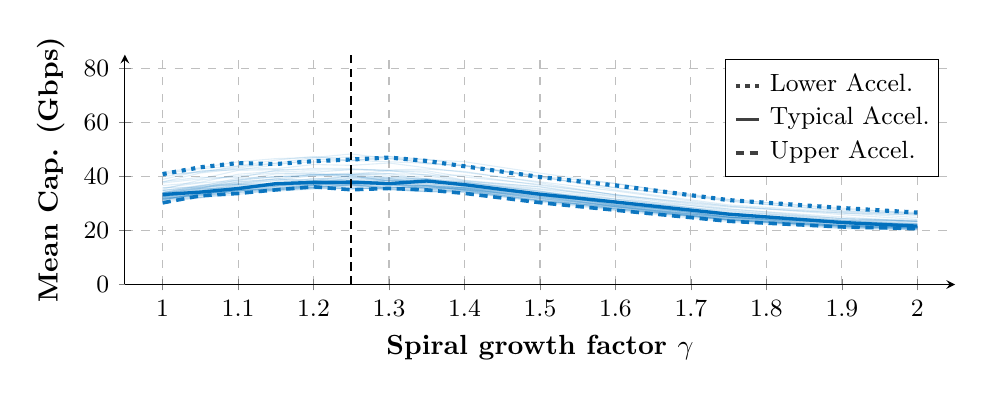
\begin{tikzpicture}
    \begin{axis}[width=\linewidth, height=4.5cm, xlabel={Spiral growth factor $\gamma$}, ylabel={Mean Cap. (Gbps)}, xmin=0.95, xmax=2.05, ymin=0, ymax=85, every axis plot/.append style={mark=none},]
            \addplot[color=cb_blue, mark=none, opacity=0.12, line width=0.4pt, solid] coordinates {(1.0,40.79) (1.05,41.47) (1.1,43.7) (1.15,44.9) (1.2,46.93) (1.25,47.08) (1.3,47.29) (1.35,44.59) (1.4,44.03) (1.5,39.55) (1.6,35.79) (1.75,30.91) (1.9,27.02) (2.0,26.19)};
            \addplot[color=cb_blue, mark=none, opacity=0.12, line width=0.4pt, solid] coordinates {(1.0,41.05) (1.05,42.83) (1.1,43.84) (1.15,46.0) (1.2,47.37) (1.25,45.78) (1.3,47.36) (1.35,46.25) (1.4,44.1) (1.5,40.04) (1.6,37.35) (1.75,30.83) (1.9,27.27) (2.0,26.21)};
            \addplot[color=cb_blue, mark=none, opacity=0.12, line width=0.4pt, solid] coordinates {(1.0,41.65) (1.05,43.16) (1.1,45.36) (1.15,46.55) (1.2,46.96) (1.25,48.28) (1.3,46.59) (1.35,46.14) (1.4,45.41) (1.5,41.18) (1.6,37.35) (1.75,31.35) (1.9,28.26) (2.0,26.26)};
            \addplot[color=cb_blue, mark=none, opacity=0.12, line width=0.4pt, solid] coordinates {(1.0,39.83) (1.05,41.9) (1.1,43.13) (1.15,44.78) (1.2,45.31) (1.25,46.0) (1.3,46.55) (1.35,45.08) (1.4,43.77) (1.5,39.79) (1.6,35.76) (1.75,31.48) (1.9,27.79) (2.0,26.65)};
            \addplot[color=cb_blue, mark=none, opacity=0.12, line width=0.4pt, solid] coordinates {(1.0,38.88) (1.05,41.93) (1.1,42.41) (1.15,44.17) (1.2,46.37) (1.25,45.86) (1.3,45.39) (1.35,44.84) (1.4,43.87) (1.5,40.08) (1.6,34.95) (1.75,29.45) (1.9,26.76) (2.0,25.65)};
            \addplot[color=cb_blue, mark=none, opacity=0.12, line width=0.4pt, solid] coordinates {(1.0,37.9) (1.05,41.22) (1.1,42.75) (1.15,42.82) (1.2,44.37) (1.25,44.07) (1.3,44.94) (1.35,43.13) (1.4,41.47) (1.5,37.97) (1.6,34.57) (1.75,28.99) (1.9,26.38) (2.0,25.74)};
            \addplot[color=cb_blue, mark=none, opacity=0.12, line width=0.4pt, solid] coordinates {(1.0,37.55) (1.05,39.03) (1.1,42.21) (1.15,42.44) (1.2,42.33) (1.25,42.5) (1.3,42.37) (1.35,42.69) (1.4,41.78) (1.5,37.59) (1.6,33.08) (1.75,28.62) (1.9,26.43) (2.0,24.81)};
            \addplot[color=cb_blue, mark=none, opacity=0.12, line width=0.4pt, solid] coordinates {(1.0,38.01) (1.05,39.65) (1.1,39.53) (1.15,42.21) (1.2,42.91) (1.25,42.87) (1.3,42.02) (1.35,42.04) (1.4,39.74) (1.5,37.02) (1.6,33.2) (1.75,28.98) (1.9,25.85) (2.0,24.09)};
            \addplot[color=cb_blue, mark=none, opacity=0.12, line width=0.4pt, solid] coordinates {(1.0,36.61) (1.05,37.77) (1.1,40.77) (1.15,41.91) (1.2,41.49) (1.25,42.47) (1.3,42.14) (1.35,40.43) (1.4,40.47) (1.5,36.68) (1.6,33.26) (1.75,27.97) (1.9,24.39) (2.0,23.82)};
            \addplot[color=cb_blue, mark=none, opacity=0.12, line width=0.4pt, solid] coordinates {(1.0,35.22) (1.05,38.66) (1.1,40.12) (1.15,41.24) (1.2,40.92) (1.25,40.66) (1.3,42.1) (1.35,41.47) (1.4,38.56) (1.5,36.06) (1.6,31.64) (1.75,27.89) (1.9,24.98) (2.0,23.25)};
            \addplot[color=cb_blue, mark=none, opacity=0.12, line width=0.4pt, solid] coordinates {(1.0,35.69) (1.05,37.57) (1.1,38.54) (1.15,40.92) (1.2,40.76) (1.25,40.58) (1.3,41.0) (1.35,40.63) (1.4,38.41) (1.5,35.4) (1.6,32.82) (1.75,27.47) (1.9,24.34) (2.0,23.48)};
            \addplot[color=cb_blue, mark=none, opacity=0.12, line width=0.4pt, solid] coordinates {(1.0,34.79) (1.05,36.68) (1.1,38.38) (1.15,40.04) (1.2,40.06) (1.25,40.29) (1.3,39.73) (1.35,40.13) (1.4,38.17) (1.5,36.18) (1.6,32.35) (1.75,26.48) (1.9,23.91) (2.0,23.48)};
            \addplot[color=cb_blue, mark=none, opacity=0.12, line width=0.4pt, solid] coordinates {(1.0,34.77) (1.05,36.32) (1.1,39.33) (1.15,39.8) (1.2,40.34) (1.25,41.22) (1.3,41.01) (1.35,39.04) (1.4,37.72) (1.5,35.16) (1.6,31.49) (1.75,26.87) (1.9,24.38) (2.0,23.36)};
            \addplot[color=cb_blue, mark=none, opacity=0.12, line width=0.4pt, solid] coordinates {(1.0,35.81) (1.05,35.94) (1.1,37.97) (1.15,38.99) (1.2,40.76) (1.25,39.78) (1.3,39.41) (1.35,39.2) (1.4,38.01) (1.5,34.58) (1.6,30.94) (1.75,27.24) (1.9,23.82) (2.0,23.37)};
            \addplot[color=cb_blue, mark=none, opacity=0.12, line width=0.4pt, solid] coordinates {(1.0,34.8) (1.05,35.59) (1.1,38.83) (1.15,39.68) (1.2,40.68) (1.25,40.85) (1.3,40.44) (1.35,38.37) (1.4,37.85) (1.5,34.22) (1.6,30.96) (1.75,25.9) (1.9,23.58) (2.0,23.34)};
            \addplot[color=cb_blue, mark=none, opacity=0.12, line width=0.4pt, solid] coordinates {(1.0,33.99) (1.05,36.59) (1.1,37.45) (1.15,38.52) (1.2,40.28) (1.25,40.61) (1.3,39.49) (1.35,39.09) (1.4,36.88) (1.5,34.05) (1.6,31.55) (1.75,26.35) (1.9,23.55) (2.0,22.86)};
            \addplot[color=cb_blue, mark=none, opacity=0.12, line width=0.4pt, solid] coordinates {(1.0,33.4) (1.05,35.98) (1.1,37.28) (1.15,39.08) (1.2,38.44) (1.25,40.26) (1.3,38.29) (1.35,37.8) (1.4,37.45) (1.5,34.46) (1.6,30.21) (1.75,25.57) (1.9,23.79) (2.0,22.14)};
            \addplot[color=cb_blue, mark=none, opacity=0.12, line width=0.4pt, solid] coordinates {(1.0,34.16) (1.05,35.87) (1.1,36.95) (1.15,38.38) (1.2,38.97) (1.25,40.02) (1.3,38.35) (1.35,38.63) (1.4,36.61) (1.5,33.82) (1.6,30.73) (1.75,25.68) (1.9,23.01) (2.0,22.6)};
            \addplot[color=cb_blue, mark=none, opacity=0.12, line width=0.4pt, solid] coordinates {(1.0,33.16) (1.05,35.47) (1.1,37.9) (1.15,39.04) (1.2,37.97) (1.25,38.48) (1.3,38.34) (1.35,38.92) (1.4,37.68) (1.5,34.53) (1.6,30.17) (1.75,25.41) (1.9,23.54) (2.0,22.47)};
            \addplot[color=cb_blue, mark=none, opacity=0.12, line width=0.4pt, solid] coordinates {(1.0,33.98) (1.05,36.3) (1.1,37.15) (1.15,37.05) (1.2,39.3) (1.25,38.54) (1.3,39.0) (1.35,38.81) (1.4,36.19) (1.5,33.14) (1.6,29.68) (1.75,25.85) (1.9,22.82) (2.0,22.3)};
            \addplot[color=cb_blue, mark=none, opacity=0.12, line width=0.4pt, solid] coordinates {(1.0,34.05) (1.05,34.8) (1.1,37.0) (1.15,37.42) (1.2,38.54) (1.25,39.59) (1.3,39.23) (1.35,37.09) (1.4,36.61) (1.5,33.31) (1.6,29.44) (1.75,26.05) (1.9,23.17) (2.0,21.85)};
            \addplot[color=cb_blue, mark=none, opacity=0.12, line width=0.4pt, solid] coordinates {(1.0,33.93) (1.05,35.25) (1.1,36.45) (1.15,36.76) (1.2,37.57) (1.25,39.37) (1.3,39.16) (1.35,37.77) (1.4,37.2) (1.5,33.67) (1.6,29.52) (1.75,25.1) (1.9,22.69) (2.0,22.45)};
            \addplot[color=cb_blue, mark=none, opacity=0.12, line width=0.4pt, solid] coordinates {(1.0,33.83) (1.05,35.6) (1.1,37.1) (1.15,36.93) (1.2,37.69) (1.25,37.65) (1.3,38.7) (1.35,38.19) (1.4,36.21) (1.5,33.54) (1.6,29.36) (1.75,25.98) (1.9,23.19) (2.0,22.41)};
            \addplot[color=cb_blue, mark=none, opacity=0.12, line width=0.4pt, solid] coordinates {(1.0,33.77) (1.05,35.54) (1.1,35.42) (1.15,37.82) (1.2,37.75) (1.25,39.13) (1.3,38.65) (1.35,38.06) (1.4,36.85) (1.5,32.86) (1.6,30.23) (1.75,24.87) (1.9,23.14) (2.0,22.22)};
            \addplot[color=cb_blue, mark=none, opacity=0.12, line width=0.4pt, solid] coordinates {(1.0,32.62) (1.05,35.24) (1.1,36.02) (1.15,36.82) (1.2,38.43) (1.25,37.59) (1.3,36.97) (1.35,36.61) (1.4,35.78) (1.5,33.68) (1.6,30.33) (1.75,24.96) (1.9,22.76) (2.0,21.6)};
            \addplot[color=cb_blue, mark=none, opacity=0.12, line width=0.4pt, solid] coordinates {(1.0,33.73) (1.05,34.61) (1.1,36.73) (1.15,36.31) (1.2,38.6) (1.25,37.34) (1.3,38.58) (1.35,36.59) (1.4,35.24) (1.5,32.83) (1.6,29.86) (1.75,24.9) (1.9,22.62) (2.0,21.63)};
            \addplot[color=cb_blue, mark=none, opacity=0.12, line width=0.4pt, solid] coordinates {(1.0,32.62) (1.05,34.54) (1.1,35.36) (1.15,37.26) (1.2,36.62) (1.25,38.6) (1.3,37.63) (1.35,37.28) (1.4,36.23) (1.5,33.08) (1.6,29.2) (1.75,24.49) (1.9,22.6) (2.0,21.35)};
            \addplot[color=cb_blue, mark=none, opacity=0.12, line width=0.4pt, solid] coordinates {(1.0,32.44) (1.05,34.93) (1.1,36.12) (1.15,36.43) (1.2,37.13) (1.25,37.55) (1.3,37.3) (1.35,36.43) (1.4,35.06) (1.5,32.61) (1.6,29.99) (1.75,25.2) (1.9,22.82) (2.0,21.62)};
            \addplot[color=cb_blue, mark=none, opacity=0.12, line width=0.4pt, solid] coordinates {(1.0,32.37) (1.05,34.38) (1.1,34.79) (1.15,36.37) (1.2,37.31) (1.25,37.82) (1.3,37.73) (1.35,36.69) (1.4,35.58) (1.5,32.23) (1.6,29.27) (1.75,25.45) (1.9,22.67) (2.0,21.11)};
            \addplot[color=cb_blue, mark=none, opacity=0.12, line width=0.4pt, solid] coordinates {(1.0,31.93) (1.05,34.22) (1.1,35.81) (1.15,36.35) (1.2,37.92) (1.25,38.03) (1.3,37.65) (1.35,36.14) (1.4,35.04) (1.5,31.83) (1.6,28.85) (1.75,24.84) (1.9,22.67) (2.0,20.94)};
            \addplot[color=cb_blue, mark=none, opacity=0.12, line width=0.4pt, solid] coordinates {(1.0,32.42) (1.05,34.37) (1.1,34.98) (1.15,36.96) (1.2,37.27) (1.25,37.03) (1.3,37.57) (1.35,35.69) (1.4,35.97) (1.5,33.0) (1.6,28.6) (1.75,24.75) (1.9,21.88) (2.0,21.86)};
            \addplot[color=cb_blue, mark=none, opacity=0.12, line width=0.4pt, solid] coordinates {(1.0,32.53) (1.05,33.32) (1.1,35.02) (1.15,37.17) (1.2,37.13) (1.25,38.01) (1.3,37.53) (1.35,37.43) (1.4,35.64) (1.5,33.24) (1.6,29.7) (1.75,24.94) (1.9,22.45) (2.0,21.34)};
            \addplot[color=cb_blue, mark=none, opacity=0.12, line width=0.4pt, solid] coordinates {(1.0,32.98) (1.05,34.11) (1.1,36.11) (1.15,36.91) (1.2,37.1) (1.25,36.93) (1.3,36.68) (1.35,36.72) (1.4,35.87) (1.5,32.48) (1.6,29.26) (1.75,24.47) (1.9,21.7) (2.0,21.07)};
            \addplot[color=cb_blue, mark=none, opacity=0.12, line width=0.4pt, solid] coordinates {(1.0,31.97) (1.05,33.61) (1.1,35.36) (1.15,35.7) (1.2,36.53) (1.25,37.62) (1.3,37.41) (1.35,35.56) (1.4,35.13) (1.5,32.41) (1.6,28.86) (1.75,24.31) (1.9,22.01) (2.0,21.66)};
            \addplot[color=cb_blue, mark=none, opacity=0.12, line width=0.4pt, solid] coordinates {(1.0,32.37) (1.05,34.13) (1.1,35.8) (1.15,36.71) (1.2,36.68) (1.25,36.22) (1.3,36.63) (1.35,36.69) (1.4,35.79) (1.5,32.96) (1.6,28.77) (1.75,24.89) (1.9,22.07) (2.0,21.27)};
            \addplot[color=cb_blue, mark=none, opacity=0.12, line width=0.4pt, solid] coordinates {(1.0,31.78) (1.05,33.33) (1.1,35.06) (1.15,35.38) (1.2,36.6) (1.25,37.47) (1.3,36.73) (1.35,35.62) (1.4,35.11) (1.5,31.63) (1.6,29.06) (1.75,24.01) (1.9,21.9) (2.0,21.23)};
            \addplot[color=cb_blue, mark=none, opacity=0.12, line width=0.4pt, solid] coordinates {(1.0,31.34) (1.05,33.91) (1.1,34.39) (1.15,36.01) (1.2,35.93) (1.25,36.76) (1.3,36.22) (1.35,35.77) (1.4,35.49) (1.5,31.91) (1.6,29.13) (1.75,24.9) (1.9,21.66) (2.0,20.63)};
            \addplot[color=cb_blue, mark=none, opacity=0.12, line width=0.4pt, solid] coordinates {(1.0,31.28) (1.05,33.67) (1.1,35.84) (1.15,35.75) (1.2,36.97) (1.25,37.44) (1.3,36.97) (1.35,36.48) (1.4,35.75) (1.5,31.56) (1.6,28.03) (1.75,24.02) (1.9,21.49) (2.0,21.21)};
            \addplot[color=cb_blue, mark=none, opacity=0.12, line width=0.4pt, solid] coordinates {(1.0,32.07) (1.05,33.06) (1.1,35.23) (1.15,36.42) (1.2,36.0) (1.25,37.03) (1.3,37.06) (1.35,35.25) (1.4,35.44) (1.5,32.71) (1.6,28.09) (1.75,23.81) (1.9,21.64) (2.0,21.17)};
            \addplot[color=cb_blue, mark=none, opacity=0.12, line width=0.4pt, solid] coordinates {(1.0,32.6) (1.05,33.25) (1.1,35.15) (1.15,35.06) (1.2,36.84) (1.25,36.95) (1.3,35.76) (1.35,36.31) (1.4,35.38) (1.5,32.03) (1.6,28.02) (1.75,24.9) (1.9,22.08) (2.0,20.76)};
            \addplot[color=cb_blue, mark=none, opacity=0.12, line width=0.4pt, solid] coordinates {(1.0,31.62) (1.05,33.06) (1.1,34.63) (1.15,35.38) (1.2,36.96) (1.25,37.15) (1.3,35.61) (1.35,36.49) (1.4,34.86) (1.5,32.25) (1.6,28.73) (1.75,24.13) (1.9,21.93) (2.0,21.31)};
            \addplot[color=cb_blue, mark=none, opacity=0.12, line width=0.4pt, solid] coordinates {(1.0,31.2) (1.05,33.61) (1.1,34.5) (1.15,35.45) (1.2,36.02) (1.25,36.78) (1.3,35.72) (1.35,36.1) (1.4,35.01) (1.5,30.91) (1.6,28.82) (1.75,23.77) (1.9,21.52) (2.0,20.83)};
            \addplot[color=cb_blue, mark=none, opacity=0.12, line width=0.4pt, solid] coordinates {(1.0,31.3) (1.05,32.25) (1.1,34.96) (1.15,34.83) (1.2,35.54) (1.25,36.82) (1.3,35.77) (1.35,36.07) (1.4,34.71) (1.5,31.14) (1.6,27.53) (1.75,24.56) (1.9,21.07) (2.0,20.9)};
            \addplot[color=cb_blue, mark=none, opacity=0.12, line width=0.4pt, solid] coordinates {(1.0,31.48) (1.05,33.46) (1.1,34.7) (1.15,35.66) (1.2,36.05) (1.25,36.82) (1.3,35.33) (1.35,34.91) (1.4,34.7) (1.5,31.19) (1.6,28.34) (1.75,24.0) (1.9,21.55) (2.0,20.6)};
            \addplot[color=cb_blue, mark=none, opacity=0.12, line width=0.4pt, solid] coordinates {(1.0,31.81) (1.05,32.67) (1.1,34.63) (1.15,34.91) (1.2,35.53) (1.25,35.51) (1.3,35.42) (1.35,34.65) (1.4,34.35) (1.5,31.83) (1.6,27.71) (1.75,23.63) (1.9,21.45) (2.0,20.86)};
            \addplot[color=cb_blue, mark=none, opacity=0.12, line width=0.4pt, solid] coordinates {(1.0,32.06) (1.05,32.88) (1.1,33.8) (1.15,34.5) (1.2,35.3) (1.25,35.58) (1.3,35.28) (1.35,34.34) (1.4,34.23) (1.5,30.96) (1.6,28.73) (1.75,23.95) (1.9,21.61) (2.0,20.17)};
            \addplot[color=cb_blue, mark=none, opacity=0.12, line width=0.4pt, solid] coordinates {(1.0,31.8) (1.05,32.74) (1.1,34.71) (1.15,35.23) (1.2,35.7) (1.25,35.87) (1.3,35.19) (1.35,34.32) (1.4,34.83) (1.5,31.19) (1.6,28.44) (1.75,23.71) (1.9,20.88) (2.0,20.63)};
            \addplot[color=cb_blue, mark=none, opacity=0.12, line width=0.4pt, solid] coordinates {(1.0,30.44) (1.05,32.08) (1.1,34.08) (1.15,34.66) (1.2,36.53) (1.25,35.19) (1.3,36.12) (1.35,35.19) (1.4,34.47) (1.5,30.71) (1.6,27.93) (1.75,23.7) (1.9,21.21) (2.0,20.81)};
            \addplot[color=cb_blue, mark=none, opacity=0.12, line width=0.4pt, solid] coordinates {(1.0,31.78) (1.05,32.21) (1.1,34.05) (1.15,35.05) (1.2,35.94) (1.25,36.53) (1.3,34.99) (1.35,34.36) (1.4,34.11) (1.5,30.48) (1.6,27.34) (1.75,23.16) (1.9,20.66) (2.0,20.31)};
            \addplot[color=cb_blue, mark=none, opacity=0.12, line width=0.4pt, solid] coordinates {(1.0,31.05) (1.05,32.07) (1.1,33.27) (1.15,35.1) (1.2,35.74) (1.25,35.52) (1.3,35.71) (1.35,35.47) (1.4,34.21) (1.5,31.1) (1.6,27.92) (1.75,24.09) (1.9,21.03) (2.0,20.33)};
            \addplot[color=cb_blue, mark=none, dotted, line width=1.5pt, opacity=0.95] coordinates {(1.0,40.81) (1.05,43.35) (1.1,44.92) (1.15,44.56) (1.2,45.6) (1.25,46.22) (1.3,46.95) (1.35,45.69) (1.4,43.73) (1.5,39.75) (1.6,36.64) (1.75,31.21) (1.9,28.29) (2.0,26.59)};
            \addplot[color=cb_blue, mark=none, solid, very thick] coordinates {(1.0,33.27) (1.05,34.17) (1.1,35.48) (1.15,37.28) (1.2,37.76) (1.25,37.86) (1.3,37.32) (1.35,38.27) (1.4,36.92) (1.5,33.4) (1.6,30.5) (1.75,26.02) (1.9,22.93) (2.0,21.59)};
            \addplot[color=cb_blue, mark=none, densely dashed, line width=1.3pt, opacity=0.95] coordinates {(1.0,30.19) (1.05,32.83) (1.1,33.67) (1.15,35.0) (1.2,36.12) (1.25,35.04) (1.3,35.53) (1.35,34.97) (1.4,33.71) (1.5,30.27) (1.6,27.48) (1.75,23.38) (1.9,21.29) (2.0,20.65)};
            \draw[densely dashed, black, line width=0.6pt] (axis cs:1.25, 0) -- (axis cs:1.25, 85);
        \node[anchor=north east, draw=black, line width=0.25pt, inner sep=3pt, fill=white, font=\small] at (rel axis cs:0.98, 0.98) {%
            \setlength{\tabcolsep}{0pt}\renewcommand{\arraystretch}{1.1}%
            \begin{tabular}{@{}c@{\hspace{3pt}}l@{}}
                \tikz[baseline=-0.5ex]{\draw[gray!50!black, dotted, line width=1.5pt] (0,0) -- (0.3cm,0);} & Lower Accel. \\
                \tikz[baseline=-0.5ex]{\draw[gray!50!black, solid, line width=1pt] (0,0) -- (0.3cm,0);} & Typical Accel. \\
                \tikz[baseline=-0.5ex]{\draw[gray!50!black, densely dashed, line width=1.3pt] (0,0) -- (0.3cm,0);} & Upper Accel. \\
            \end{tabular}%
        };
    \end{axis}
\end{tikzpicture}
        \vspace{-25pt}
        \caption{Translational}
    \end{subfigure}
    \hfill
    \begin{subfigure}{0.495\linewidth}
        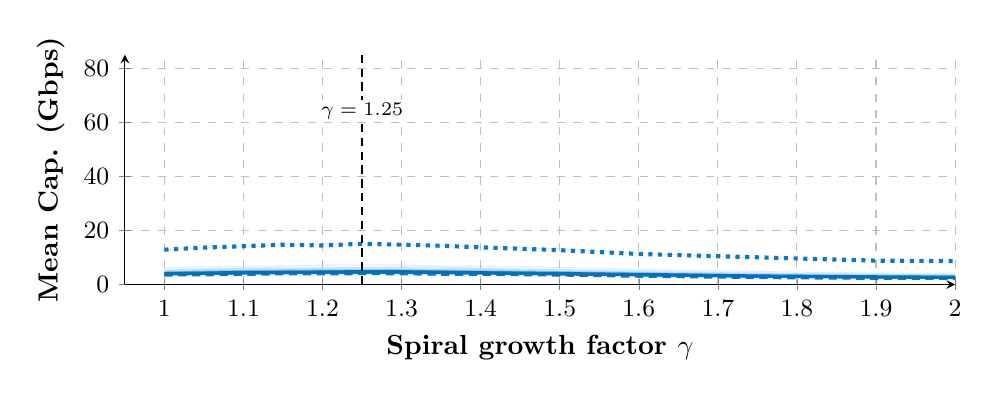
\begin{tikzpicture}
    \begin{axis}[width=\linewidth, height=4.5cm, xlabel={Spiral growth factor $\gamma$}, ylabel={Mean Cap. (Gbps)}, xmin=0.95, xmax=2, ymin=0, ymax=85, every axis plot/.append style={mark=none},]
            \addplot[color=cb_blue, mark=none, opacity=0.12, line width=0.4pt, solid] coordinates {(1.0,12.77) (1.05,13.64) (1.1,13.91) (1.15,14.8) (1.2,14.98) (1.25,14.88) (1.3,14.72) (1.35,14.35) (1.4,13.93) (1.5,13.19) (1.6,11.49) (1.75,9.84) (1.9,9.02) (2.0,8.52)};
            \addplot[color=cb_blue, mark=none, opacity=0.12, line width=0.4pt, solid] coordinates {(1.0,6.23) (1.05,6.49) (1.1,6.68) (1.15,6.94) (1.2,7.21) (1.25,7.21) (1.3,7.21) (1.35,6.88) (1.4,6.8) (1.5,6.35) (1.6,5.55) (1.75,4.79) (1.9,4.17) (2.0,4.18)};
            \addplot[color=cb_blue, mark=none, opacity=0.12, line width=0.4pt, solid] coordinates {(1.0,5.63) (1.05,5.8) (1.1,6.0) (1.15,6.31) (1.2,6.43) (1.25,6.32) (1.3,6.57) (1.35,6.42) (1.4,6.1) (1.5,5.49) (1.6,5.1) (1.75,4.27) (1.9,3.87) (2.0,3.68)};
            \addplot[color=cb_blue, mark=none, opacity=0.12, line width=0.4pt, solid] coordinates {(1.0,5.28) (1.05,5.7) (1.1,5.97) (1.15,5.93) (1.2,6.13) (1.25,6.12) (1.3,6.24) (1.35,6.01) (1.4,5.94) (1.5,5.44) (1.6,4.73) (1.75,4.13) (1.9,3.63) (2.0,3.58)};
            \addplot[color=cb_blue, mark=none, opacity=0.12, line width=0.4pt, solid] coordinates {(1.0,5.11) (1.05,5.44) (1.1,5.51) (1.15,5.68) (1.2,5.87) (1.25,6.03) (1.3,5.85) (1.35,5.64) (1.4,5.59) (1.5,5.07) (1.6,4.59) (1.75,3.91) (1.9,3.48) (2.0,3.32)};
            \addplot[color=cb_blue, mark=none, opacity=0.12, line width=0.4pt, solid] coordinates {(1.0,4.82) (1.05,5.18) (1.1,5.36) (1.15,5.43) (1.2,5.68) (1.25,5.51) (1.3,5.67) (1.35,5.56) (1.4,5.42) (1.5,4.87) (1.6,4.42) (1.75,3.79) (1.9,3.42) (2.0,3.21)};
            \addplot[color=cb_blue, mark=none, opacity=0.12, line width=0.4pt, solid] coordinates {(1.0,4.67) (1.05,5.02) (1.1,5.24) (1.15,5.47) (1.2,5.58) (1.25,5.49) (1.3,5.48) (1.35,5.36) (1.4,5.28) (1.5,4.76) (1.6,4.32) (1.75,3.58) (1.9,3.26) (2.0,3.21)};
            \addplot[color=cb_blue, mark=none, opacity=0.12, line width=0.4pt, solid] coordinates {(1.0,4.65) (1.05,4.96) (1.1,5.15) (1.15,5.36) (1.2,5.46) (1.25,5.5) (1.3,5.33) (1.35,5.22) (1.4,5.17) (1.5,4.75) (1.6,4.28) (1.75,3.49) (1.9,3.13) (2.0,3.1)};
            \addplot[color=cb_blue, mark=none, opacity=0.12, line width=0.4pt, solid] coordinates {(1.0,4.69) (1.05,4.94) (1.1,5.08) (1.15,5.15) (1.2,5.16) (1.25,5.33) (1.3,5.36) (1.35,5.15) (1.4,5.06) (1.5,4.69) (1.6,4.02) (1.75,3.56) (1.9,3.11) (2.0,3.0)};
            \addplot[color=cb_blue, mark=none, opacity=0.12, line width=0.4pt, solid] coordinates {(1.0,4.45) (1.05,4.76) (1.1,4.96) (1.15,5.17) (1.2,5.1) (1.25,5.11) (1.3,5.28) (1.35,5.12) (1.4,4.88) (1.5,4.62) (1.6,3.99) (1.75,3.45) (1.9,3.06) (2.0,2.94)};
            \addplot[color=cb_blue, mark=none, opacity=0.12, line width=0.4pt, solid] coordinates {(1.0,4.38) (1.05,4.78) (1.1,5.0) (1.15,5.09) (1.2,5.05) (1.25,5.16) (1.3,5.1) (1.35,5.07) (1.4,4.93) (1.5,4.47) (1.6,3.97) (1.75,3.48) (1.9,3.02) (2.0,2.93)};
            \addplot[color=cb_blue, mark=none, opacity=0.12, line width=0.4pt, solid] coordinates {(1.0,4.43) (1.05,4.59) (1.1,4.85) (1.15,5.0) (1.2,5.2) (1.25,5.05) (1.3,5.2) (1.35,5.02) (1.4,4.78) (1.5,4.45) (1.6,4.01) (1.75,3.42) (1.9,2.96) (2.0,2.92)};
            \addplot[color=cb_blue, mark=none, opacity=0.12, line width=0.4pt, solid] coordinates {(1.0,4.38) (1.05,4.69) (1.1,4.73) (1.15,5.0) (1.2,5.04) (1.25,5.01) (1.3,5.05) (1.35,4.95) (1.4,4.82) (1.5,4.43) (1.6,3.96) (1.75,3.4) (1.9,3.01) (2.0,2.93)};
            \addplot[color=cb_blue, mark=none, opacity=0.12, line width=0.4pt, solid] coordinates {(1.0,4.34) (1.05,4.47) (1.1,4.68) (1.15,4.86) (1.2,4.99) (1.25,4.86) (1.3,4.88) (1.35,4.9) (1.4,4.62) (1.5,4.23) (1.6,3.86) (1.75,3.36) (1.9,2.95) (2.0,2.88)};
            \addplot[color=cb_blue, mark=none, opacity=0.12, line width=0.4pt, solid] coordinates {(1.0,4.34) (1.05,4.43) (1.1,4.74) (1.15,4.8) (1.2,4.97) (1.25,4.98) (1.3,4.85) (1.35,4.71) (1.4,4.77) (1.5,4.2) (1.6,3.92) (1.75,3.32) (1.9,2.95) (2.0,2.87)};
            \addplot[color=cb_blue, mark=none, opacity=0.12, line width=0.4pt, solid] coordinates {(1.0,4.32) (1.05,4.5) (1.1,4.58) (1.15,4.82) (1.2,4.72) (1.25,4.88) (1.3,4.83) (1.35,4.79) (1.4,4.65) (1.5,4.24) (1.6,3.85) (1.75,3.29) (1.9,2.83) (2.0,2.74)};
            \addplot[color=cb_blue, mark=none, opacity=0.12, line width=0.4pt, solid] coordinates {(1.0,4.08) (1.05,4.47) (1.1,4.58) (1.15,4.8) (1.2,4.72) (1.25,4.71) (1.3,4.86) (1.35,4.8) (1.4,4.52) (1.5,4.16) (1.6,3.68) (1.75,3.26) (1.9,2.83) (2.0,2.74)};
            \addplot[color=cb_blue, mark=none, opacity=0.12, line width=0.4pt, solid] coordinates {(1.0,4.06) (1.05,4.43) (1.1,4.44) (1.15,4.64) (1.2,4.78) (1.25,4.83) (1.3,4.85) (1.35,4.64) (1.4,4.57) (1.5,4.07) (1.6,3.7) (1.75,3.1) (1.9,2.83) (2.0,2.71)};
            \addplot[color=cb_blue, mark=none, opacity=0.12, line width=0.4pt, solid] coordinates {(1.0,4.2) (1.05,4.21) (1.1,4.45) (1.15,4.6) (1.2,4.81) (1.25,4.82) (1.3,4.61) (1.35,4.66) (1.4,4.49) (1.5,4.21) (1.6,3.65) (1.75,3.12) (1.9,2.76) (2.0,2.64)};
            \addplot[color=cb_blue, mark=none, opacity=0.12, line width=0.4pt, solid] coordinates {(1.0,4.15) (1.05,4.26) (1.1,4.48) (1.15,4.61) (1.2,4.69) (1.25,4.58) (1.3,4.73) (1.35,4.52) (1.4,4.36) (1.5,4.09) (1.6,3.57) (1.75,3.15) (1.9,2.74) (2.0,2.64)};
            \addplot[color=cb_blue, mark=none, opacity=0.12, line width=0.4pt, solid] coordinates {(1.0,4.12) (1.05,4.21) (1.1,4.34) (1.15,4.64) (1.2,4.52) (1.25,4.75) (1.3,4.55) (1.35,4.47) (1.4,4.36) (1.5,3.98) (1.6,3.66) (1.75,3.01) (1.9,2.7) (2.0,2.7)};
            \addplot[color=cb_blue, mark=none, opacity=0.12, line width=0.4pt, solid] coordinates {(1.0,3.97) (1.05,4.18) (1.1,4.32) (1.15,4.42) (1.2,4.66) (1.25,4.64) (1.3,4.66) (1.35,4.52) (1.4,4.45) (1.5,4.03) (1.6,3.54) (1.75,3.07) (1.9,2.81) (2.0,2.58)};
            \addplot[color=cb_blue, mark=none, opacity=0.12, line width=0.4pt, solid] coordinates {(1.0,4.07) (1.05,4.28) (1.1,4.38) (1.15,4.5) (1.2,4.7) (1.25,4.52) (1.3,4.59) (1.35,4.49) (1.4,4.42) (1.5,4.01) (1.6,3.67) (1.75,3.0) (1.9,2.68) (2.0,2.65)};
            \addplot[color=cb_blue, mark=none, opacity=0.12, line width=0.4pt, solid] coordinates {(1.0,3.91) (1.05,4.14) (1.1,4.39) (1.15,4.5) (1.2,4.53) (1.25,4.71) (1.3,4.58) (1.35,4.48) (1.4,4.38) (1.5,3.91) (1.6,3.61) (1.75,3.1) (1.9,2.75) (2.0,2.66)};
            \addplot[color=cb_blue, mark=none, opacity=0.12, line width=0.4pt, solid] coordinates {(1.0,4.02) (1.05,4.11) (1.1,4.33) (1.15,4.41) (1.2,4.51) (1.25,4.57) (1.3,4.53) (1.35,4.38) (1.4,4.32) (1.5,4.01) (1.6,3.54) (1.75,2.98) (1.9,2.77) (2.0,2.55)};
            \addplot[color=cb_blue, mark=none, opacity=0.12, line width=0.4pt, solid] coordinates {(1.0,4.02) (1.05,4.06) (1.1,4.23) (1.15,4.5) (1.2,4.6) (1.25,4.57) (1.3,4.55) (1.35,4.46) (1.4,4.28) (1.5,3.88) (1.6,3.52) (1.75,3.04) (1.9,2.74) (2.0,2.64)};
            \addplot[color=cb_blue, mark=none, opacity=0.12, line width=0.4pt, solid] coordinates {(1.0,3.98) (1.05,4.22) (1.1,4.31) (1.15,4.39) (1.2,4.52) (1.25,4.47) (1.3,4.54) (1.35,4.36) (1.4,4.21) (1.5,4.0) (1.6,3.5) (1.75,3.04) (1.9,2.7) (2.0,2.62)};
            \addplot[color=cb_blue, mark=none, opacity=0.12, line width=0.4pt, solid] coordinates {(1.0,3.98) (1.05,4.2) (1.1,4.34) (1.15,4.42) (1.2,4.51) (1.25,4.4) (1.3,4.58) (1.35,4.47) (1.4,4.22) (1.5,3.85) (1.6,3.54) (1.75,2.96) (1.9,2.65) (2.0,2.51)};
            \addplot[color=cb_blue, mark=none, opacity=0.12, line width=0.4pt, solid] coordinates {(1.0,3.97) (1.05,4.1) (1.1,4.23) (1.15,4.3) (1.2,4.49) (1.25,4.38) (1.3,4.51) (1.35,4.31) (1.4,4.23) (1.5,3.86) (1.6,3.47) (1.75,3.0) (1.9,2.7) (2.0,2.56)};
            \addplot[color=cb_blue, mark=none, opacity=0.12, line width=0.4pt, solid] coordinates {(1.0,3.79) (1.05,3.97) (1.1,4.15) (1.15,4.38) (1.2,4.47) (1.25,4.41) (1.3,4.47) (1.35,4.35) (1.4,4.21) (1.5,3.83) (1.6,3.51) (1.75,2.9) (1.9,2.64) (2.0,2.51)};
            \addplot[color=cb_blue, mark=none, opacity=0.12, line width=0.4pt, solid] coordinates {(1.0,3.88) (1.05,4.04) (1.1,4.24) (1.15,4.23) (1.2,4.38) (1.25,4.46) (1.3,4.3) (1.35,4.28) (1.4,4.14) (1.5,3.78) (1.6,3.41) (1.75,2.91) (1.9,2.57) (2.0,2.56)};
            \addplot[color=cb_blue, mark=none, opacity=0.12, line width=0.4pt, solid] coordinates {(1.0,3.77) (1.05,3.99) (1.1,4.22) (1.15,4.3) (1.2,4.46) (1.25,4.48) (1.3,4.29) (1.35,4.38) (1.4,4.08) (1.5,3.74) (1.6,3.5) (1.75,2.97) (1.9,2.63) (2.0,2.52)};
            \addplot[color=cb_blue, mark=none, opacity=0.12, line width=0.4pt, solid] coordinates {(1.0,3.85) (1.05,3.98) (1.1,4.07) (1.15,4.18) (1.2,4.32) (1.25,4.45) (1.3,4.38) (1.35,4.35) (1.4,4.24) (1.5,3.73) (1.6,3.47) (1.75,2.87) (1.9,2.61) (2.0,2.5)};
            \addplot[color=cb_blue, mark=none, opacity=0.12, line width=0.4pt, solid] coordinates {(1.0,3.76) (1.05,3.93) (1.1,4.1) (1.15,4.22) (1.2,4.26) (1.25,4.36) (1.3,4.25) (1.35,4.26) (1.4,4.21) (1.5,3.76) (1.6,3.43) (1.75,2.93) (1.9,2.63) (2.0,2.45)};
            \addplot[color=cb_blue, mark=none, opacity=0.12, line width=0.4pt, solid] coordinates {(1.0,3.7) (1.05,3.89) (1.1,4.13) (1.15,4.28) (1.2,4.34) (1.25,4.26) (1.3,4.37) (1.35,4.23) (1.4,4.16) (1.5,3.81) (1.6,3.36) (1.75,2.93) (1.9,2.58) (2.0,2.49)};
            \addplot[color=cb_blue, mark=none, opacity=0.12, line width=0.4pt, solid] coordinates {(1.0,3.76) (1.05,3.99) (1.1,4.11) (1.15,4.13) (1.2,4.19) (1.25,4.3) (1.3,4.24) (1.35,4.16) (1.4,3.99) (1.5,3.74) (1.6,3.32) (1.75,2.85) (1.9,2.5) (2.0,2.5)};
            \addplot[color=cb_blue, mark=none, opacity=0.12, line width=0.4pt, solid] coordinates {(1.0,3.64) (1.05,3.97) (1.1,4.13) (1.15,4.2) (1.2,4.26) (1.25,4.28) (1.3,4.27) (1.35,4.24) (1.4,4.14) (1.5,3.71) (1.6,3.38) (1.75,2.86) (1.9,2.52) (2.0,2.44)};
            \addplot[color=cb_blue, mark=none, opacity=0.12, line width=0.4pt, solid] coordinates {(1.0,3.63) (1.05,3.79) (1.1,3.96) (1.15,4.24) (1.2,4.2) (1.25,4.31) (1.3,4.24) (1.35,4.09) (1.4,3.99) (1.5,3.69) (1.6,3.3) (1.75,2.83) (1.9,2.48) (2.0,2.41)};
            \addplot[color=cb_blue, mark=none, opacity=0.12, line width=0.4pt, solid] coordinates {(1.0,3.64) (1.05,3.84) (1.1,3.98) (1.15,4.16) (1.2,4.27) (1.25,4.27) (1.3,4.12) (1.35,4.05) (1.4,4.05) (1.5,3.64) (1.6,3.33) (1.75,2.83) (1.9,2.56) (2.0,2.46)};
            \addplot[color=cb_blue, mark=none, opacity=0.12, line width=0.4pt, solid] coordinates {(1.0,3.63) (1.05,3.85) (1.1,3.92) (1.15,4.08) (1.2,4.29) (1.25,4.26) (1.3,4.17) (1.35,4.13) (1.4,4.08) (1.5,3.62) (1.6,3.26) (1.75,2.83) (1.9,2.54) (2.0,2.42)};
            \addplot[color=cb_blue, mark=none, opacity=0.12, line width=0.4pt, solid] coordinates {(1.0,3.7) (1.05,3.86) (1.1,4.01) (1.15,4.1) (1.2,4.2) (1.25,4.18) (1.3,4.14) (1.35,4.07) (1.4,3.91) (1.5,3.59) (1.6,3.34) (1.75,2.78) (1.9,2.45) (2.0,2.35)};
            \addplot[color=cb_blue, mark=none, opacity=0.12, line width=0.4pt, solid] coordinates {(1.0,3.55) (1.05,3.87) (1.1,3.87) (1.15,4.13) (1.2,4.22) (1.25,4.25) (1.3,4.05) (1.35,4.04) (1.4,4.01) (1.5,3.56) (1.6,3.23) (1.75,2.72) (1.9,2.52) (2.0,2.41)};
            \addplot[color=cb_blue, mark=none, opacity=0.12, line width=0.4pt, solid] coordinates {(1.0,3.66) (1.05,3.72) (1.1,3.92) (1.15,4.03) (1.2,4.16) (1.25,4.1) (1.3,4.12) (1.35,4.01) (1.4,3.98) (1.5,3.6) (1.6,3.24) (1.75,2.72) (1.9,2.5) (2.0,2.36)};
            \addplot[color=cb_blue, mark=none, opacity=0.12, line width=0.4pt, solid] coordinates {(1.0,3.65) (1.05,3.74) (1.1,4.0) (1.15,4.13) (1.2,4.1) (1.25,4.09) (1.3,4.08) (1.35,4.04) (1.4,4.01) (1.5,3.64) (1.6,3.26) (1.75,2.69) (1.9,2.42) (2.0,2.37)};
            \addplot[color=cb_blue, mark=none, opacity=0.12, line width=0.4pt, solid] coordinates {(1.0,3.64) (1.05,3.76) (1.1,3.82) (1.15,4.09) (1.2,4.16) (1.25,4.07) (1.3,4.15) (1.35,3.97) (1.4,3.98) (1.5,3.51) (1.6,3.19) (1.75,2.79) (1.9,2.41) (2.0,2.34)};
            \addplot[color=cb_blue, mark=none, opacity=0.12, line width=0.4pt, solid] coordinates {(1.0,3.53) (1.05,3.64) (1.1,3.8) (1.15,4.0) (1.2,4.02) (1.25,4.2) (1.3,4.05) (1.35,3.91) (1.4,3.97) (1.5,3.62) (1.6,3.21) (1.75,2.75) (1.9,2.39) (2.0,2.31)};
            \addplot[color=cb_blue, mark=none, opacity=0.12, line width=0.4pt, solid] coordinates {(1.0,3.6) (1.05,3.75) (1.1,3.8) (1.15,4.03) (1.2,4.05) (1.25,3.98) (1.3,3.97) (1.35,3.94) (1.4,3.93) (1.5,3.55) (1.6,3.21) (1.75,2.71) (1.9,2.38) (2.0,2.3)};
            \addplot[color=cb_blue, mark=none, opacity=0.12, line width=0.4pt, solid] coordinates {(1.0,3.5) (1.05,3.62) (1.1,3.84) (1.15,4.03) (1.2,4.03) (1.25,3.99) (1.3,4.12) (1.35,3.99) (1.4,3.76) (1.5,3.53) (1.6,3.12) (1.75,2.65) (1.9,2.4) (2.0,2.33)};
            \addplot[color=cb_blue, mark=none, opacity=0.12, line width=0.4pt, solid] coordinates {(1.0,3.47) (1.05,3.68) (1.1,3.87) (1.15,3.88) (1.2,4.13) (1.25,3.97) (1.3,4.04) (1.35,3.96) (1.4,3.94) (1.5,3.53) (1.6,3.14) (1.75,2.68) (1.9,2.42) (2.0,2.37)};
            \addplot[color=cb_blue, mark=none, opacity=0.12, line width=0.4pt, solid] coordinates {(1.0,3.47) (1.05,3.59) (1.1,3.88) (1.15,3.91) (1.2,4.06) (1.25,4.07) (1.3,4.07) (1.35,3.99) (1.4,3.8) (1.5,3.43) (1.6,3.15) (1.75,2.72) (1.9,2.36) (2.0,2.34)};
            \addplot[color=cb_blue, mark=none, dotted, line width=1.5pt, opacity=0.95] coordinates {(1.0,12.86) (1.05,13.64) (1.1,14.15) (1.15,14.71) (1.2,14.43) (1.25,15.05) (1.3,14.72) (1.35,14.33) (1.4,13.74) (1.5,12.69) (1.6,11.28) (1.75,10.04) (1.9,8.81) (2.0,8.66)};
            \addplot[color=cb_blue, mark=none, solid, very thick] coordinates {(1.0,4.03) (1.05,4.17) (1.1,4.45) (1.15,4.45) (1.2,4.58) (1.25,4.7) (1.3,4.69) (1.35,4.49) (1.4,4.31) (1.5,4.0) (1.6,3.68) (1.75,3.11) (1.9,2.8) (2.0,2.63)};
            \addplot[color=cb_blue, mark=none, densely dashed, line width=1.3pt, opacity=0.95] coordinates {(1.0,3.59) (1.05,3.68) (1.1,3.83) (1.15,4.03) (1.2,4.02) (1.25,4.1) (1.3,4.06) (1.35,3.86) (1.4,3.85) (1.5,3.57) (1.6,3.15) (1.75,2.65) (1.9,2.35) (2.0,2.32)};
            \draw[densely dashed, black, line width=0.6pt] (axis cs:1.25, 0) -- (axis cs:1.25, 85);
            \node[anchor=south, font=\scriptsize, fill=white, inner sep=1pt] at (axis cs:1.25, 60) {$\gamma=1.25$};
    \end{axis}
\end{tikzpicture}
        \vspace{-25pt}
        \caption{Rotational}
    \end{subfigure}
    \vspace{-5pt}
    \caption{Spiral growth factor $\gamma$ parameter sensitivity for Hierarchical Search ($d_{\text{link}} = 3$~m, Ideal Mechanical). Lower, Typical, and Upper Acceleration values are bolded: $0.5$, $9.5$, and $20$ m/s$^2$ (translational); $0.5$, $300$, and $700$ deg/s$^2$ (rotational).}
    \vspace{-5pt}
    \label{fig:reb_tuning_hs}
\end{figure}

\begin{figure}[ht!]
    \centering
    \begin{subfigure}{0.495\linewidth}
        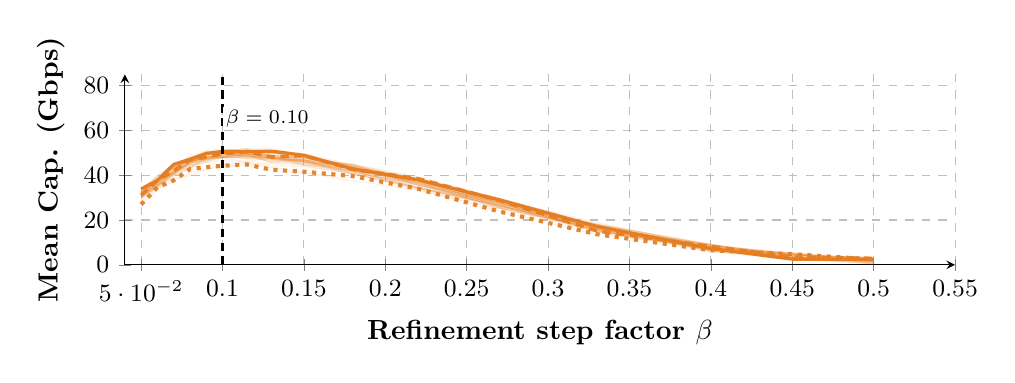
\begin{tikzpicture}
    \begin{axis}[
        width=\linewidth, height=4cm,
        xlabel={Refinement step factor $\beta$},
        ylabel={Mean Cap. (Gbps)},
        xmin=0.04, xmax=0.55,
        ymin=0, ymax=85,
        every axis plot/.append style={mark=none},
    ]
            \addplot[color=cb_orange, mark=none, opacity=0.12, line width=0.4pt, solid] coordinates {(0.05,28.73) (0.06,34.44) (0.07,38.59) (0.08,39.75) (0.09,42.29) (0.1,44.10) (0.115,44.66) (0.13,43.50) (0.15,41.23) (0.18,37.48) (0.22,33.33) (0.27,24.89) (0.33,16.15) (0.4,6.87) (0.45,3.49) (0.5,0.32)};
            \addplot[color=cb_orange, mark=none, opacity=0.12, line width=0.4pt, solid] coordinates {(0.05,27.25) (0.06,33.46) (0.07,37.58) (0.08,40.90) (0.09,42.68) (0.1,44.75) (0.115,45.59) (0.13,44.16) (0.15,43.91) (0.18,40.77) (0.22,33.77) (0.27,23.91) (0.33,13.56) (0.4,7.77) (0.45,3.47) (0.5,2.12)};
            \addplot[color=cb_orange, mark=none, opacity=0.12, line width=0.4pt, solid] coordinates {(0.05,31.18) (0.06,33.97) (0.07,39.92) (0.08,43.77) (0.09,45.67) (0.1,46.52) (0.115,45.81) (0.13,45.12) (0.15,44.73) (0.18,41.92) (0.22,33.99) (0.27,26.24) (0.33,14.90) (0.4,8.70) (0.45,4.72) (0.5,1.87)};
            \addplot[color=cb_orange, mark=none, opacity=0.12, line width=0.4pt, solid] coordinates {(0.05,30.85) (0.06,35.76) (0.07,40.61) (0.08,46.63) (0.09,47.18) (0.1,48.36) (0.115,49.79) (0.13,48.00) (0.15,46.07) (0.18,42.08) (0.22,34.86) (0.27,26.15) (0.33,17.08) (0.4,7.96) (0.45,4.73) (0.5,0.77)};
            \addplot[color=cb_orange, mark=none, opacity=0.12, line width=0.4pt, solid] coordinates {(0.05,31.73) (0.06,38.51) (0.07,41.73) (0.08,46.52) (0.09,47.05) (0.1,49.22) (0.115,49.37) (0.13,47.41) (0.15,45.57) (0.18,43.30) (0.22,36.73) (0.27,25.69) (0.33,18.20) (0.4,9.09) (0.45,3.78) (0.5,0.49)};
            \addplot[color=cb_orange, mark=none, opacity=0.12, line width=0.4pt, solid] coordinates {(0.05,33.21) (0.06,37.61) (0.07,43.36) (0.08,46.59) (0.09,48.32) (0.1,49.99) (0.115,51.44) (0.13,48.17) (0.15,47.65) (0.18,43.39) (0.22,38.60) (0.27,27.54) (0.33,18.08) (0.4,9.06) (0.45,3.20) (0.5,2.85)};
            \addplot[color=cb_orange, mark=none, opacity=0.12, line width=0.4pt, solid] coordinates {(0.05,32.56) (0.06,40.13) (0.07,43.71) (0.08,48.89) (0.09,49.58) (0.1,51.26) (0.115,51.33) (0.13,52.11) (0.15,48.64) (0.18,43.65) (0.22,38.21) (0.27,27.66) (0.33,17.37) (0.4,8.14) (0.45,3.92) (0.5,1.24)};
            \addplot[color=cb_orange, mark=none, opacity=0.12, line width=0.4pt, solid] coordinates {(0.05,31.72) (0.06,39.24) (0.07,43.90) (0.08,46.74) (0.09,51.30) (0.1,51.21) (0.115,51.85) (0.13,51.00) (0.15,49.75) (0.18,44.46) (0.22,38.62) (0.27,29.34) (0.33,18.89) (0.4,7.96) (0.45,2.42) (0.5,1.89)};
            \addplot[color=cb_orange, mark=none, opacity=0.12, line width=0.4pt, solid] coordinates {(0.05,33.12) (0.06,39.81) (0.07,44.93) (0.08,47.43) (0.09,50.34) (0.1,51.15) (0.115,51.71) (0.13,49.89) (0.15,49.13) (0.18,43.58) (0.22,37.88) (0.27,29.83) (0.33,16.57) (0.4,8.66) (0.45,4.61) (0.5,3.14)};
            \addplot[color=cb_orange, mark=none, opacity=0.12, line width=0.4pt, solid] coordinates {(0.05,33.82) (0.06,39.49) (0.07,42.85) (0.08,46.65) (0.09,50.67) (0.1,50.79) (0.115,51.88) (0.13,48.20) (0.15,46.70) (0.18,44.97) (0.22,39.22) (0.27,29.72) (0.33,17.90) (0.4,7.68) (0.45,2.61) (0.5,2.34)};
            \addplot[color=cb_orange, mark=none, opacity=0.12, line width=0.4pt, solid] coordinates {(0.05,33.51) (0.06,37.59) (0.07,43.48) (0.08,48.19) (0.09,47.74) (0.1,50.22) (0.115,49.26) (0.13,48.85) (0.15,46.45) (0.18,44.11) (0.22,37.53) (0.27,28.67) (0.33,15.67) (0.4,6.34) (0.45,5.30) (0.5,2.26)};
            \addplot[color=cb_orange, mark=none, opacity=0.12, line width=0.4pt, solid] coordinates {(0.05,30.97) (0.06,38.84) (0.07,41.12) (0.08,46.16) (0.09,47.98) (0.1,49.71) (0.115,47.77) (0.13,49.85) (0.15,48.60) (0.18,44.17) (0.22,35.73) (0.27,27.16) (0.33,16.13) (0.4,8.05) (0.45,4.44) (0.5,1.56)};
            \addplot[color=cb_orange, mark=none, opacity=0.12, line width=0.4pt, solid] coordinates {(0.05,30.66) (0.06,38.18) (0.07,40.86) (0.08,45.39) (0.09,48.24) (0.1,49.16) (0.115,49.18) (0.13,48.51) (0.15,48.38) (0.18,42.37) (0.22,38.15) (0.27,27.60) (0.33,15.70) (0.4,7.88) (0.45,4.55) (0.5,2.64)};
            \addplot[color=cb_orange, mark=none, opacity=0.12, line width=0.4pt, solid] coordinates {(0.05,29.73) (0.06,37.06) (0.07,41.55) (0.08,46.80) (0.09,47.18) (0.1,48.77) (0.115,48.91) (0.13,47.37) (0.15,46.78) (0.18,43.14) (0.22,36.83) (0.27,27.60) (0.33,16.89) (0.4,8.75) (0.45,4.32) (0.5,3.17)};
            \addplot[color=cb_orange, mark=none, opacity=0.12, line width=0.4pt, solid] coordinates {(0.05,31.55) (0.06,35.79) (0.07,41.07) (0.08,45.38) (0.09,48.36) (0.1,48.43) (0.115,47.51) (0.13,48.38) (0.15,44.89) (0.18,41.18) (0.22,36.10) (0.27,28.25) (0.33,16.34) (0.4,8.94) (0.45,4.97) (0.5,0.95)};
            \addplot[color=cb_orange, mark=none, opacity=0.12, line width=0.4pt, solid] coordinates {(0.05,32.04) (0.06,36.25) (0.07,42.16) (0.08,45.78) (0.09,46.86) (0.1,48.26) (0.115,49.60) (0.13,46.16) (0.15,47.41) (0.18,43.50) (0.22,36.60) (0.27,28.18) (0.33,17.76) (0.4,8.55) (0.45,3.39) (0.5,2.75)};
            \addplot[color=cb_orange, mark=none, opacity=0.12, line width=0.4pt, solid] coordinates {(0.05,29.37) (0.06,36.52) (0.07,41.07) (0.08,45.63) (0.09,48.10) (0.1,48.37) (0.115,49.24) (0.13,48.97) (0.15,44.61) (0.18,41.48) (0.22,34.31) (0.27,27.92) (0.33,16.42) (0.4,8.94) (0.45,2.91) (0.5,0.29)};
            \addplot[color=cb_orange, mark=none, opacity=0.12, line width=0.4pt, solid] coordinates {(0.05,32.00) (0.06,37.66) (0.07,40.41) (0.08,44.59) (0.09,46.14) (0.1,48.21) (0.115,47.33) (0.13,47.30) (0.15,44.42) (0.18,43.55) (0.22,34.57) (0.27,26.38) (0.33,16.74) (0.4,8.33) (0.45,5.34) (0.5,1.49)};
            \addplot[color=cb_orange, mark=none, opacity=0.12, line width=0.4pt, solid] coordinates {(0.05,31.64) (0.06,35.01) (0.07,40.68) (0.08,43.43) (0.09,47.20) (0.1,48.08) (0.115,49.38) (0.13,45.62) (0.15,45.22) (0.18,41.93) (0.22,37.22) (0.27,27.66) (0.33,14.77) (0.4,8.11) (0.45,3.98) (0.5,3.37)};
            \addplot[color=cb_orange, mark=none, opacity=0.12, line width=0.4pt, solid] coordinates {(0.05,30.22) (0.06,35.68) (0.07,39.75) (0.08,43.32) (0.09,48.19) (0.1,47.87) (0.115,48.19) (0.13,47.46) (0.15,45.79) (0.18,40.34) (0.22,36.51) (0.27,25.49) (0.33,14.79) (0.4,7.67) (0.45,2.36) (0.5,2.64)};
            \addplot[color=cb_orange, mark=none, opacity=0.12, line width=0.4pt, solid] coordinates {(0.05,29.66) (0.06,35.00) (0.07,41.95) (0.08,43.93) (0.09,45.76) (0.1,47.78) (0.115,45.90) (0.13,48.10) (0.15,44.19) (0.18,40.62) (0.22,34.65) (0.27,25.21) (0.33,16.56) (0.4,5.86) (0.45,2.18) (0.5,2.72)};
            \addplot[color=cb_orange, mark=none, opacity=0.12, line width=0.4pt, solid] coordinates {(0.05,29.77) (0.06,35.38) (0.07,39.64) (0.08,43.02) (0.09,47.77) (0.1,47.80) (0.115,48.40) (0.13,46.84) (0.15,46.32) (0.18,41.92) (0.22,34.19) (0.27,26.32) (0.33,17.51) (0.4,5.92) (0.45,4.75) (0.5,2.98)};
            \addplot[color=cb_orange, mark=none, opacity=0.12, line width=0.4pt, solid] coordinates {(0.05,30.75) (0.06,35.86) (0.07,42.32) (0.08,43.09) (0.09,46.93) (0.1,47.84) (0.115,48.24) (0.13,46.93) (0.15,46.80) (0.18,40.49) (0.22,34.12) (0.27,26.69) (0.33,14.58) (0.4,6.70) (0.45,4.25) (0.5,1.92)};
            \addplot[color=cb_orange, mark=none, opacity=0.12, line width=0.4pt, solid] coordinates {(0.05,30.09) (0.06,37.66) (0.07,40.88) (0.08,44.41) (0.09,47.36) (0.1,47.85) (0.115,48.30) (0.13,48.15) (0.15,45.95) (0.18,42.82) (0.22,36.28) (0.27,25.38) (0.33,15.88) (0.4,6.54) (0.45,3.27) (0.5,1.60)};
            \addplot[color=cb_orange, mark=none, opacity=0.12, line width=0.4pt, solid] coordinates {(0.05,30.40) (0.06,34.65) (0.07,40.53) (0.08,45.12) (0.09,46.59) (0.1,47.85) (0.115,49.04) (0.13,45.52) (0.15,46.55) (0.18,40.56) (0.22,34.18) (0.27,27.14) (0.33,17.08) (0.4,7.64) (0.45,4.10) (0.5,1.96)};
            \addplot[color=cb_orange, mark=none, opacity=0.12, line width=0.4pt, solid] coordinates {(0.05,30.15) (0.06,34.78) (0.07,40.34) (0.08,45.18) (0.09,47.91) (0.1,47.91) (0.115,48.43) (0.13,48.60) (0.15,45.83) (0.18,41.48) (0.22,35.84) (0.27,25.41) (0.33,16.59) (0.4,6.54) (0.45,2.50) (0.5,2.92)};
            \addplot[color=cb_orange, mark=none, opacity=0.12, line width=0.4pt, solid] coordinates {(0.05,30.48) (0.06,37.18) (0.07,41.36) (0.08,45.97) (0.09,48.56) (0.1,48.24) (0.115,49.09) (0.13,47.73) (0.15,46.29) (0.18,40.67) (0.22,37.27) (0.27,27.66) (0.33,15.39) (0.4,6.43) (0.45,4.52) (0.5,1.12)};
            \addplot[color=cb_orange, mark=none, opacity=0.12, line width=0.4pt, solid] coordinates {(0.05,30.50) (0.06,34.75) (0.07,42.51) (0.08,45.31) (0.09,47.22) (0.1,48.41) (0.115,48.64) (0.13,45.93) (0.15,46.81) (0.18,41.45) (0.22,35.68) (0.27,26.11) (0.33,15.79) (0.4,8.29) (0.45,4.79) (0.5,2.00)};
            \addplot[color=cb_orange, mark=none, opacity=0.12, line width=0.4pt, solid] coordinates {(0.05,29.80) (0.06,35.10) (0.07,40.31) (0.08,45.74) (0.09,48.42) (0.1,48.68) (0.115,49.01) (0.13,47.73) (0.15,46.03) (0.18,41.88) (0.22,37.02) (0.27,25.48) (0.33,16.08) (0.4,6.84) (0.45,4.48) (0.5,1.74)};
            \addplot[color=cb_orange, mark=none, opacity=0.12, line width=0.4pt, solid] coordinates {(0.05,31.78) (0.06,35.08) (0.07,41.13) (0.08,45.68) (0.09,46.14) (0.1,48.68) (0.115,47.47) (0.13,46.55) (0.15,45.40) (0.18,42.06) (0.22,34.48) (0.27,27.64) (0.33,15.21) (0.4,7.17) (0.45,4.57) (0.5,1.79)};
            \addplot[color=cb_orange, mark=none, opacity=0.12, line width=0.4pt, solid] coordinates {(0.05,32.53) (0.06,37.88) (0.07,40.25) (0.08,46.83) (0.09,46.52) (0.1,48.95) (0.115,50.17) (0.13,49.29) (0.15,46.75) (0.18,43.14) (0.22,37.07) (0.27,26.66) (0.33,15.09) (0.4,5.98) (0.45,3.30) (0.5,2.83)};
            \addplot[color=cb_orange, mark=none, opacity=0.12, line width=0.4pt, solid] coordinates {(0.05,32.04) (0.06,38.27) (0.07,43.49) (0.08,44.53) (0.09,49.66) (0.1,49.34) (0.115,49.42) (0.13,48.51) (0.15,46.50) (0.18,42.57) (0.22,36.09) (0.27,26.58) (0.33,15.39) (0.4,7.72) (0.45,2.59) (0.5,1.84)};
            \addplot[color=cb_orange, mark=none, opacity=0.12, line width=0.4pt, solid] coordinates {(0.05,33.29) (0.06,36.88) (0.07,43.15) (0.08,47.41) (0.09,49.93) (0.1,49.71) (0.115,48.25) (0.13,47.74) (0.15,47.56) (0.18,44.46) (0.22,37.46) (0.27,26.24) (0.33,17.61) (0.4,7.72) (0.45,4.84) (0.5,2.73)};
            \addplot[color=cb_orange, mark=none, opacity=0.12, line width=0.4pt, solid] coordinates {(0.05,31.82) (0.06,39.04) (0.07,42.76) (0.08,46.96) (0.09,49.47) (0.1,49.91) (0.115,50.12) (0.13,47.77) (0.15,45.89) (0.18,43.53) (0.22,36.38) (0.27,26.68) (0.33,15.18) (0.4,7.80) (0.45,3.31) (0.5,1.66)};
            \addplot[color=cb_orange, mark=none, opacity=0.12, line width=0.4pt, solid] coordinates {(0.05,30.45) (0.06,38.71) (0.07,41.05) (0.08,47.76) (0.09,50.27) (0.1,49.91) (0.115,49.70) (0.13,48.86) (0.15,47.59) (0.18,44.75) (0.22,38.45) (0.27,27.29) (0.33,17.81) (0.4,8.30) (0.45,3.35) (0.5,1.75)};
            \addplot[color=cb_orange, mark=none, opacity=0.12, line width=0.4pt, solid] coordinates {(0.05,30.74) (0.06,35.97) (0.07,41.09) (0.08,47.81) (0.09,48.42) (0.1,49.84) (0.115,49.62) (0.13,47.78) (0.15,46.45) (0.18,43.45) (0.22,36.80) (0.27,27.51) (0.33,15.52) (0.4,7.32) (0.45,3.21) (0.5,1.51)};
            \addplot[color=cb_orange, mark=none, opacity=0.12, line width=0.4pt, solid] coordinates {(0.05,31.34) (0.06,37.78) (0.07,43.41) (0.08,46.86) (0.09,47.37) (0.1,49.76) (0.115,50.15) (0.13,48.09) (0.15,48.03) (0.18,44.14) (0.22,38.37) (0.27,28.69) (0.33,16.10) (0.4,8.04) (0.45,2.71) (0.5,1.30)};
            \addplot[color=cb_orange, mark=none, opacity=0.12, line width=0.4pt, solid] coordinates {(0.05,33.51) (0.06,38.11) (0.07,42.00) (0.08,46.65) (0.09,50.38) (0.1,49.73) (0.115,49.07) (0.13,49.83) (0.15,48.32) (0.18,44.16) (0.22,38.08) (0.27,28.20) (0.33,17.32) (0.4,7.84) (0.45,4.47) (0.5,1.56)};
            \addplot[color=cb_orange, mark=none, opacity=0.12, line width=0.4pt, solid] coordinates {(0.05,31.40) (0.06,36.94) (0.07,41.26) (0.08,45.32) (0.09,50.41) (0.1,49.73) (0.115,48.55) (0.13,47.55) (0.15,45.75) (0.18,44.77) (0.22,35.54) (0.27,28.31) (0.33,17.84) (0.4,9.08) (0.45,2.35) (0.5,1.26)};
            \addplot[color=cb_orange, mark=none, opacity=0.12, line width=0.4pt, solid] coordinates {(0.05,32.78) (0.06,36.10) (0.07,41.91) (0.08,45.10) (0.09,49.96) (0.1,49.68) (0.115,50.52) (0.13,47.60) (0.15,46.96) (0.18,43.22) (0.22,37.51) (0.27,26.43) (0.33,16.46) (0.4,6.99) (0.45,4.82) (0.5,1.64)};
            \addplot[color=cb_orange, mark=none, opacity=0.12, line width=0.4pt, solid] coordinates {(0.05,31.95) (0.06,36.69) (0.07,43.37) (0.08,46.12) (0.09,49.93) (0.1,49.64) (0.115,50.96) (0.13,50.41) (0.15,47.01) (0.18,42.73) (0.22,36.46) (0.27,27.42) (0.33,18.26) (0.4,8.83) (0.45,5.00) (0.5,0.56)};
            \addplot[color=cb_orange, mark=none, opacity=0.12, line width=0.4pt, solid] coordinates {(0.05,30.93) (0.06,37.80) (0.07,43.56) (0.08,46.38) (0.09,47.34) (0.1,49.59) (0.115,50.58) (0.13,47.93) (0.15,48.01) (0.18,42.66) (0.22,38.24) (0.27,26.07) (0.33,16.41) (0.4,9.27) (0.45,2.98) (0.5,1.65)};
            \addplot[color=cb_orange, mark=none, opacity=0.12, line width=0.4pt, solid] coordinates {(0.05,31.29) (0.06,35.69) (0.07,40.73) (0.08,46.22) (0.09,47.83) (0.1,49.62) (0.115,48.96) (0.13,47.07) (0.15,48.62) (0.18,44.65) (0.22,37.37) (0.27,28.32) (0.33,15.37) (0.4,6.99) (0.45,5.09) (0.5,2.50)};
            \addplot[color=cb_orange, mark=none, opacity=0.12, line width=0.4pt, solid] coordinates {(0.05,30.54) (0.06,38.03) (0.07,42.08) (0.08,44.47) (0.09,47.26) (0.1,49.59) (0.115,50.52) (0.13,48.85) (0.15,47.88) (0.18,43.54) (0.22,35.48) (0.27,26.56) (0.33,15.93) (0.4,6.15) (0.45,3.67) (0.5,2.84)};
            \addplot[color=cb_orange, mark=none, opacity=0.12, line width=0.4pt, solid] coordinates {(0.05,31.65) (0.06,35.97) (0.07,43.67) (0.08,46.53) (0.09,47.05) (0.1,49.60) (0.115,48.47) (0.13,47.45) (0.15,46.86) (0.18,43.86) (0.22,35.94) (0.27,27.01) (0.33,17.20) (0.4,6.29) (0.45,5.60) (0.5,0.32)};
            \addplot[color=cb_orange, mark=none, opacity=0.12, line width=0.4pt, solid] coordinates {(0.05,31.90) (0.06,37.35) (0.07,43.97) (0.08,46.39) (0.09,48.36) (0.1,49.61) (0.115,49.85) (0.13,50.37) (0.15,46.26) (0.18,41.79) (0.22,37.85) (0.27,26.77) (0.33,17.44) (0.4,8.17) (0.45,4.89) (0.5,2.64)};
            \addplot[color=cb_orange, mark=none, opacity=0.12, line width=0.4pt, solid] coordinates {(0.05,31.20) (0.06,35.71) (0.07,42.39) (0.08,47.25) (0.09,47.56) (0.1,49.56) (0.115,49.21) (0.13,49.32) (0.15,47.52) (0.18,44.50) (0.22,35.29) (0.27,28.24) (0.33,16.47) (0.4,7.00) (0.45,2.36) (0.5,0.77)};
            \addplot[color=cb_orange, mark=none, dotted, line width=1.5pt, opacity=0.95] coordinates {(0.05,26.92) (0.06,34.60) (0.07,37.71) (0.08,42.68) (0.09,43.55) (0.1,44.20) (0.115,44.78) (0.13,42.43) (0.15,41.53) (0.18,39.59) (0.22,33.96) (0.27,23.81) (0.33,13.65) (0.4,6.48) (0.45,4.72) (0.5,2.37)};
            \addplot[color=cb_orange, mark=none, solid, very thick] coordinates {(0.05,33.83) (0.06,37.66) (0.07,44.78) (0.08,47.09) (0.09,49.68) (0.1,50.58) (0.115,50.41) (0.13,50.71) (0.15,48.84) (0.18,42.82) (0.22,37.93) (0.27,28.98) (0.33,17.12) (0.4,7.24) (0.45,2.54) (0.5,2.42)};
            \addplot[color=cb_orange, mark=none, densely dashed, line width=1.3pt, opacity=0.95] coordinates {(0.05,31.08) (0.06,37.62) (0.07,41.94) (0.08,46.78) (0.09,48.13) (0.1,49.52) (0.115,50.57) (0.13,48.10) (0.15,48.75) (0.18,42.60) (0.22,38.44) (0.27,28.81) (0.33,15.13) (0.4,8.19) (0.45,3.47) (0.5,2.86)};

            \draw[densely dashed, black, line width=0.8pt] (axis cs:0.10, 0) -- (axis cs:0.10, 85);
            \node[anchor=south west, font=\scriptsize, fill=white, inner sep=1pt] at (axis cs:0.10, 60) {$\beta=0.10$};
    \end{axis}
\end{tikzpicture}

        \vspace{-25pt}
        \caption{Translational}
    \end{subfigure}
    \hfill
    \begin{subfigure}{0.495\linewidth}
        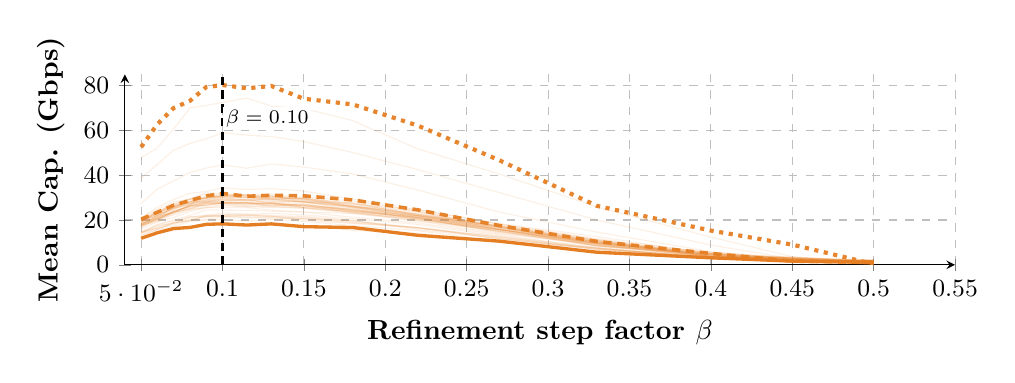
\begin{tikzpicture}
    \begin{axis}[
        width=\linewidth, height=4cm,
        xlabel={Refinement step factor $\beta$},
        ylabel={Mean Cap. (Gbps)},
        xmin=0.04, xmax=0.55,
        ymin=0, ymax=85,
        every axis plot/.append style={mark=none},
    ]
            \addplot[color=cb_orange, mark=none, opacity=0.12, line width=0.4pt, solid] coordinates {(0.05,47.87) (0.06,52.16) (0.07,60.63) (0.08,70.02) (0.09,71.17) (0.1,72.50) (0.115,74.40) (0.13,70.82) (0.15,69.76) (0.18,64.34) (0.22,51.74) (0.27,40.51) (0.33,25.82) (0.4,12.37) (0.45,3.65) (0.5,0.90)};
            \addplot[color=cb_orange, mark=none, opacity=0.12, line width=0.4pt, solid] coordinates {(0.05,38.65) (0.06,44.89) (0.07,51.20) (0.08,54.12) (0.09,56.26) (0.1,58.92) (0.115,57.86) (0.13,57.26) (0.15,55.00) (0.18,50.11) (0.22,42.47) (0.27,32.22) (0.33,19.98) (0.4,8.80) (0.45,2.73) (0.5,1.56)};
            \addplot[color=cb_orange, mark=none, opacity=0.12, line width=0.4pt, solid] coordinates {(0.05,27.33) (0.06,33.87) (0.07,37.47) (0.08,41.19) (0.09,43.17) (0.1,44.61) (0.115,43.11) (0.13,45.04) (0.15,43.63) (0.18,40.58) (0.22,33.35) (0.27,23.52) (0.33,14.58) (0.4,5.82) (0.45,2.93) (0.5,1.61)};
            \addplot[color=cb_orange, mark=none, opacity=0.12, line width=0.4pt, solid] coordinates {(0.05,20.97) (0.06,25.69) (0.07,29.08) (0.08,31.95) (0.09,32.73) (0.1,34.35) (0.115,33.58) (0.13,34.02) (0.15,32.85) (0.18,29.36) (0.22,24.57) (0.27,18.44) (0.33,12.59) (0.4,4.95) (0.45,3.02) (0.5,1.99)};
            \addplot[color=cb_orange, mark=none, opacity=0.12, line width=0.4pt, solid] coordinates {(0.05,17.23) (0.06,20.28) (0.07,23.94) (0.08,26.19) (0.09,27.81) (0.1,27.38) (0.115,26.91) (0.13,27.73) (0.15,25.43) (0.18,23.63) (0.22,21.22) (0.27,15.97) (0.33,8.78) (0.4,4.64) (0.45,2.16) (0.5,1.15)};
            \addplot[color=cb_orange, mark=none, opacity=0.12, line width=0.4pt, solid] coordinates {(0.05,13.29) (0.06,15.86) (0.07,18.64) (0.08,19.70) (0.09,20.37) (0.1,21.32) (0.115,21.36) (0.13,21.00) (0.15,20.52) (0.18,18.75) (0.22,16.51) (0.27,11.68) (0.33,7.46) (0.4,3.23) (0.45,1.39) (0.5,1.07)};
            \addplot[color=cb_orange, mark=none, opacity=0.12, line width=0.4pt, solid] coordinates {(0.05,12.04) (0.06,14.03) (0.07,15.35) (0.08,16.90) (0.09,18.00) (0.1,18.15) (0.115,18.27) (0.13,18.09) (0.15,17.60) (0.18,15.36) (0.22,14.10) (0.27,9.96) (0.33,5.96) (0.4,2.84) (0.45,1.98) (0.5,0.91)};
            \addplot[color=cb_orange, mark=none, opacity=0.12, line width=0.4pt, solid] coordinates {(0.05,13.01) (0.06,15.60) (0.07,17.01) (0.08,19.36) (0.09,19.89) (0.1,20.19) (0.115,19.51) (0.13,20.20) (0.15,19.40) (0.18,17.48) (0.22,15.20) (0.27,10.47) (0.33,7.45) (0.4,3.40) (0.45,1.46) (0.5,1.10)};
            \addplot[color=cb_orange, mark=none, opacity=0.12, line width=0.4pt, solid] coordinates {(0.05,14.74) (0.06,16.36) (0.07,17.90) (0.08,20.01) (0.09,21.51) (0.1,21.88) (0.115,21.90) (0.13,21.59) (0.15,20.70) (0.18,19.00) (0.22,16.67) (0.27,12.18) (0.33,7.34) (0.4,3.17) (0.45,1.01) (0.5,0.20)};
            \addplot[color=cb_orange, mark=none, opacity=0.12, line width=0.4pt, solid] coordinates {(0.05,14.21) (0.06,17.55) (0.07,18.46) (0.08,21.52) (0.09,21.41) (0.1,22.37) (0.115,22.20) (0.13,21.50) (0.15,21.22) (0.18,19.56) (0.22,16.52) (0.27,12.62) (0.33,7.22) (0.4,3.17) (0.45,2.27) (0.5,0.22)};
            \addplot[color=cb_orange, mark=none, opacity=0.12, line width=0.4pt, solid] coordinates {(0.05,14.40) (0.06,16.50) (0.07,18.70) (0.08,19.64) (0.09,21.98) (0.1,21.63) (0.115,21.04) (0.13,20.72) (0.15,20.63) (0.18,19.65) (0.22,15.66) (0.27,11.76) (0.33,6.77) (0.4,3.58) (0.45,1.62) (0.5,0.08)};
            \addplot[color=cb_orange, mark=none, opacity=0.12, line width=0.4pt, solid] coordinates {(0.05,14.09) (0.06,15.87) (0.07,18.63) (0.08,20.04) (0.09,21.63) (0.1,21.70) (0.115,21.98) (0.13,21.77) (0.15,19.94) (0.18,18.41) (0.22,16.68) (0.27,11.47) (0.33,7.01) (0.4,3.32) (0.45,1.37) (0.5,1.35)};
            \addplot[color=cb_orange, mark=none, opacity=0.12, line width=0.4pt, solid] coordinates {(0.05,14.30) (0.06,16.95) (0.07,19.10) (0.08,20.89) (0.09,21.98) (0.1,22.24) (0.115,22.67) (0.13,22.01) (0.15,21.61) (0.18,19.81) (0.22,16.20) (0.27,12.42) (0.33,6.81) (0.4,2.89) (0.45,1.17) (0.5,0.51)};
            \addplot[color=cb_orange, mark=none, opacity=0.12, line width=0.4pt, solid] coordinates {(0.05,14.32) (0.06,17.72) (0.07,19.74) (0.08,21.42) (0.09,22.15) (0.1,23.14) (0.115,22.52) (0.13,22.93) (0.15,22.29) (0.18,20.51) (0.22,17.99) (0.27,12.83) (0.33,7.74) (0.4,3.02) (0.45,1.54) (0.5,0.77)};
            \addplot[color=cb_orange, mark=none, opacity=0.12, line width=0.4pt, solid] coordinates {(0.05,14.87) (0.06,18.10) (0.07,19.94) (0.08,22.09) (0.09,24.49) (0.1,24.38) (0.115,24.28) (0.13,23.92) (0.15,23.47) (0.18,21.22) (0.22,18.69) (0.27,13.40) (0.33,7.46) (0.4,3.00) (0.45,2.39) (0.5,0.54)};
            \addplot[color=cb_orange, mark=none, opacity=0.12, line width=0.4pt, solid] coordinates {(0.05,15.98) (0.06,19.29) (0.07,21.18) (0.08,23.72) (0.09,25.53) (0.1,25.55) (0.115,25.52) (0.13,24.39) (0.15,23.57) (0.18,22.88) (0.22,19.55) (0.27,13.82) (0.33,9.14) (0.4,3.16) (0.45,2.42) (0.5,1.02)};
            \addplot[color=cb_orange, mark=none, opacity=0.12, line width=0.4pt, solid] coordinates {(0.05,17.73) (0.06,19.02) (0.07,22.98) (0.08,24.91) (0.09,25.42) (0.1,26.25) (0.115,26.04) (0.13,25.49) (0.15,25.51) (0.18,22.89) (0.22,20.40) (0.27,14.95) (0.33,8.32) (0.4,4.66) (0.45,2.25) (0.5,0.69)};
            \addplot[color=cb_orange, mark=none, opacity=0.12, line width=0.4pt, solid] coordinates {(0.05,17.61) (0.06,20.45) (0.07,22.25) (0.08,24.33) (0.09,25.83) (0.1,26.85) (0.115,25.90) (0.13,26.07) (0.15,25.09) (0.18,23.60) (0.22,19.61) (0.27,15.16) (0.33,8.60) (0.4,3.74) (0.45,2.81) (0.5,1.90)};
            \addplot[color=cb_orange, mark=none, opacity=0.12, line width=0.4pt, solid] coordinates {(0.05,17.74) (0.06,19.64) (0.07,24.00) (0.08,25.81) (0.09,27.45) (0.1,27.13) (0.115,27.70) (0.13,25.92) (0.15,26.46) (0.18,23.29) (0.22,20.55) (0.27,15.56) (0.33,9.59) (0.4,4.56) (0.45,2.14) (0.5,1.14)};
            \addplot[color=cb_orange, mark=none, opacity=0.12, line width=0.4pt, solid] coordinates {(0.05,17.31) (0.06,20.67) (0.07,23.50) (0.08,26.05) (0.09,27.94) (0.1,27.69) (0.115,27.59) (0.13,26.75) (0.15,27.14) (0.18,24.01) (0.22,21.44) (0.27,14.91) (0.33,8.32) (0.4,4.84) (0.45,2.65) (0.5,1.46)};
            \addplot[color=cb_orange, mark=none, opacity=0.12, line width=0.4pt, solid] coordinates {(0.05,17.79) (0.06,21.29) (0.07,23.47) (0.08,25.11) (0.09,27.45) (0.1,27.87) (0.115,27.60) (0.13,26.79) (0.15,26.02) (0.18,25.06) (0.22,20.38) (0.27,15.49) (0.33,9.47) (0.4,4.31) (0.45,1.91) (0.5,1.38)};
            \addplot[color=cb_orange, mark=none, opacity=0.12, line width=0.4pt, solid] coordinates {(0.05,16.92) (0.06,20.11) (0.07,24.21) (0.08,25.78) (0.09,26.54) (0.1,27.76) (0.115,27.52) (0.13,26.28) (0.15,27.25) (0.18,23.74) (0.22,20.98) (0.27,14.56) (0.33,9.60) (0.4,3.66) (0.45,3.05) (0.5,0.58)};
            \addplot[color=cb_orange, mark=none, opacity=0.12, line width=0.4pt, solid] coordinates {(0.05,18.00) (0.06,20.29) (0.07,23.28) (0.08,26.50) (0.09,26.48) (0.1,27.61) (0.115,27.11) (0.13,27.49) (0.15,25.71) (0.18,24.49) (0.22,20.90) (0.27,14.23) (0.33,9.21) (0.4,3.59) (0.45,1.67) (0.5,1.36)};
            \addplot[color=cb_orange, mark=none, opacity=0.12, line width=0.4pt, solid] coordinates {(0.05,16.61) (0.06,20.97) (0.07,23.93) (0.08,26.43) (0.09,26.74) (0.1,27.37) (0.115,26.42) (0.13,26.64) (0.15,26.43) (0.18,23.22) (0.22,19.97) (0.27,15.79) (0.33,8.48) (0.4,4.79) (0.45,2.66) (0.5,0.30)};
            \addplot[color=cb_orange, mark=none, opacity=0.12, line width=0.4pt, solid] coordinates {(0.05,18.59) (0.06,20.01) (0.07,23.50) (0.08,24.68) (0.09,27.31) (0.1,27.51) (0.115,27.81) (0.13,27.25) (0.15,25.45) (0.18,23.93) (0.22,20.79) (0.27,15.83) (0.33,8.43) (0.4,3.52) (0.45,2.68) (0.5,1.18)};
            \addplot[color=cb_orange, mark=none, opacity=0.12, line width=0.4pt, solid] coordinates {(0.05,17.57) (0.06,21.79) (0.07,23.30) (0.08,25.15) (0.09,26.84) (0.1,27.76) (0.115,27.74) (0.13,27.44) (0.15,26.57) (0.18,24.86) (0.22,20.99) (0.27,15.96) (0.33,9.61) (0.4,3.94) (0.45,2.24) (0.5,1.04)};
            \addplot[color=cb_orange, mark=none, opacity=0.12, line width=0.4pt, solid] coordinates {(0.05,18.47) (0.06,20.70) (0.07,23.03) (0.08,26.91) (0.09,28.45) (0.1,28.05) (0.115,27.16) (0.13,27.53) (0.15,26.82) (0.18,24.63) (0.22,21.77) (0.27,16.39) (0.33,10.25) (0.4,3.65) (0.45,2.94) (0.5,1.16)};
            \addplot[color=cb_orange, mark=none, opacity=0.12, line width=0.4pt, solid] coordinates {(0.05,18.11) (0.06,21.93) (0.07,24.95) (0.08,27.60) (0.09,28.70) (0.1,28.66) (0.115,27.66) (0.13,27.65) (0.15,26.29) (0.18,24.23) (0.22,21.86) (0.27,15.79) (0.33,9.87) (0.4,4.47) (0.45,2.11) (0.5,1.46)};
            \addplot[color=cb_orange, mark=none, opacity=0.12, line width=0.4pt, solid] coordinates {(0.05,17.91) (0.06,22.10) (0.07,25.18) (0.08,26.80) (0.09,28.36) (0.1,29.27) (0.115,28.53) (0.13,29.36) (0.15,27.87) (0.18,25.42) (0.22,22.01) (0.27,16.80) (0.33,10.18) (0.4,3.67) (0.45,2.74) (0.5,1.54)};
            \addplot[color=cb_orange, mark=none, opacity=0.12, line width=0.4pt, solid] coordinates {(0.05,20.26) (0.06,21.97) (0.07,25.07) (0.08,28.22) (0.09,29.81) (0.1,30.45) (0.115,29.90) (0.13,30.40) (0.15,29.43) (0.18,25.87) (0.22,23.06) (0.27,17.19) (0.33,9.49) (0.4,5.71) (0.45,2.47) (0.5,1.72)};
            \addplot[color=cb_orange, mark=none, opacity=0.12, line width=0.4pt, solid] coordinates {(0.05,20.21) (0.06,22.44) (0.07,25.43) (0.08,29.27) (0.09,29.74) (0.1,30.78) (0.115,31.22) (0.13,29.20) (0.15,29.89) (0.18,26.48) (0.22,21.92) (0.27,17.40) (0.33,10.48) (0.4,3.88) (0.45,2.35) (0.5,0.83)};
            \addplot[color=cb_orange, mark=none, opacity=0.12, line width=0.4pt, solid] coordinates {(0.05,19.88) (0.06,23.47) (0.07,26.13) (0.08,28.34) (0.09,29.59) (0.1,31.00) (0.115,31.34) (0.13,29.84) (0.15,29.46) (0.18,26.17) (0.22,23.81) (0.27,16.51) (0.33,10.33) (0.4,4.57) (0.45,1.71) (0.5,2.07)};
            \addplot[color=cb_orange, mark=none, opacity=0.12, line width=0.4pt, solid] coordinates {(0.05,20.50) (0.06,23.27) (0.07,27.11) (0.08,29.18) (0.09,30.05) (0.1,30.77) (0.115,30.45) (0.13,30.68) (0.15,28.73) (0.18,26.05) (0.22,22.58) (0.27,16.94) (0.33,11.18) (0.4,4.10) (0.45,3.10) (0.5,2.17)};
            \addplot[color=cb_orange, mark=none, opacity=0.12, line width=0.4pt, solid] coordinates {(0.05,20.65) (0.06,22.16) (0.07,26.07) (0.08,28.11) (0.09,30.88) (0.1,30.68) (0.115,30.65) (0.13,29.06) (0.15,28.49) (0.18,27.02) (0.22,22.36) (0.27,17.15) (0.33,10.21) (0.4,4.98) (0.45,2.43) (0.5,1.71)};
            \addplot[color=cb_orange, mark=none, opacity=0.12, line width=0.4pt, solid] coordinates {(0.05,18.89) (0.06,23.78) (0.07,26.52) (0.08,27.83) (0.09,28.88) (0.1,30.47) (0.115,29.76) (0.13,29.58) (0.15,29.66) (0.18,27.50) (0.22,23.59) (0.27,15.71) (0.33,10.55) (0.4,5.49) (0.45,2.91) (0.5,0.27)};
            \addplot[color=cb_orange, mark=none, opacity=0.12, line width=0.4pt, solid] coordinates {(0.05,19.22) (0.06,21.94) (0.07,25.45) (0.08,26.91) (0.09,30.39) (0.1,29.88) (0.115,28.89) (0.13,30.21) (0.15,29.21) (0.18,26.22) (0.22,22.61) (0.27,16.18) (0.33,11.01) (0.4,3.79) (0.45,1.53) (0.5,0.33)};
            \addplot[color=cb_orange, mark=none, opacity=0.12, line width=0.4pt, solid] coordinates {(0.05,19.27) (0.06,20.99) (0.07,24.88) (0.08,26.91) (0.09,29.47) (0.1,29.04) (0.115,28.42) (0.13,28.13) (0.15,28.19) (0.18,25.85) (0.22,22.05) (0.27,15.61) (0.33,9.27) (0.4,3.66) (0.45,1.71) (0.5,1.63)};
            \addplot[color=cb_orange, mark=none, opacity=0.12, line width=0.4pt, solid] coordinates {(0.05,18.40) (0.06,20.71) (0.07,23.57) (0.08,26.42) (0.09,27.75) (0.1,28.44) (0.115,29.23) (0.13,27.33) (0.15,26.63) (0.18,24.45) (0.22,20.36) (0.27,14.97) (0.33,9.90) (0.4,5.08) (0.45,2.66) (0.5,0.13)};
            \addplot[color=cb_orange, mark=none, opacity=0.12, line width=0.4pt, solid] coordinates {(0.05,19.10) (0.06,21.28) (0.07,23.67) (0.08,26.26) (0.09,27.94) (0.1,28.74) (0.115,28.96) (0.13,27.73) (0.15,28.28) (0.18,24.24) (0.22,21.15) (0.27,15.72) (0.33,10.13) (0.4,3.97) (0.45,2.21) (0.5,1.67)};
            \addplot[color=cb_orange, mark=none, opacity=0.12, line width=0.4pt, solid] coordinates {(0.05,18.02) (0.06,21.02) (0.07,25.61) (0.08,28.24) (0.09,27.99) (0.1,29.26) (0.115,28.86) (0.13,28.99) (0.15,28.08) (0.18,25.80) (0.22,21.24) (0.27,16.75) (0.33,8.83) (0.4,3.67) (0.45,3.15) (0.5,0.96)};
            \addplot[color=cb_orange, mark=none, opacity=0.12, line width=0.4pt, solid] coordinates {(0.05,18.33) (0.06,23.27) (0.07,26.08) (0.08,27.40) (0.09,28.32) (0.1,29.80) (0.115,28.97) (0.13,29.41) (0.15,28.97) (0.18,25.89) (0.22,21.15) (0.27,16.78) (0.33,9.31) (0.4,4.05) (0.45,1.72) (0.5,0.63)};
            \addplot[color=cb_orange, mark=none, opacity=0.12, line width=0.4pt, solid] coordinates {(0.05,20.03) (0.06,21.58) (0.07,25.80) (0.08,27.39) (0.09,29.02) (0.1,29.98) (0.115,29.95) (0.13,28.51) (0.15,28.01) (0.18,25.51) (0.22,21.63) (0.27,17.31) (0.33,10.10) (0.4,4.94) (0.45,3.02) (0.5,1.72)};
            \addplot[color=cb_orange, mark=none, opacity=0.12, line width=0.4pt, solid] coordinates {(0.05,20.49) (0.06,23.42) (0.07,25.55) (0.08,28.34) (0.09,29.76) (0.1,30.33) (0.115,30.19) (0.13,29.53) (0.15,28.12) (0.18,26.19) (0.22,21.93) (0.27,17.53) (0.33,10.76) (0.4,3.79) (0.45,3.46) (0.5,1.17)};
            \addplot[color=cb_orange, mark=none, opacity=0.12, line width=0.4pt, solid] coordinates {(0.05,20.12) (0.06,24.01) (0.07,26.99) (0.08,27.54) (0.09,30.29) (0.1,30.49) (0.115,31.02) (0.13,30.82) (0.15,28.01) (0.18,27.77) (0.22,22.04) (0.27,17.52) (0.33,10.86) (0.4,4.44) (0.45,3.15) (0.5,1.85)};
            \addplot[color=cb_orange, mark=none, opacity=0.12, line width=0.4pt, solid] coordinates {(0.05,19.24) (0.06,23.61) (0.07,27.18) (0.08,29.40) (0.09,31.46) (0.1,31.11) (0.115,31.40) (0.13,31.51) (0.15,29.68) (0.18,27.39) (0.22,22.43) (0.27,18.19) (0.33,11.26) (0.4,4.83) (0.45,2.06) (0.5,1.12)};
            \addplot[color=cb_orange, mark=none, opacity=0.12, line width=0.4pt, solid] coordinates {(0.05,19.27) (0.06,23.08) (0.07,26.19) (0.08,29.36) (0.09,29.81) (0.1,31.46) (0.115,30.66) (0.13,30.07) (0.15,30.35) (0.18,28.49) (0.22,24.12) (0.27,16.93) (0.33,9.49) (0.4,5.09) (0.45,3.42) (0.5,1.76)};
            \addplot[color=cb_orange, mark=none, opacity=0.12, line width=0.4pt, solid] coordinates {(0.05,21.15) (0.06,24.71) (0.07,28.11) (0.08,29.32) (0.09,32.20) (0.1,31.78) (0.115,30.75) (0.13,30.75) (0.15,29.37) (0.18,27.08) (0.22,24.60) (0.27,18.14) (0.33,11.68) (0.4,5.28) (0.45,1.80) (0.5,2.21)};
            \addplot[color=cb_orange, mark=none, dotted, line width=1.5pt, opacity=0.95] coordinates {(0.05,52.54) (0.06,62.78) (0.07,69.99) (0.08,73.18) (0.09,79.33) (0.1,80.24) (0.115,78.78) (0.13,79.82) (0.15,74.11) (0.18,71.59) (0.22,62.11) (0.27,46.68) (0.33,26.29) (0.4,15.27) (0.45,9.00) (0.5,0.32)};
            \addplot[color=cb_orange, mark=none, solid, very thick] coordinates {(0.05,11.85) (0.06,14.29) (0.07,16.18) (0.08,16.67) (0.09,18.04) (0.1,18.28) (0.115,17.74) (0.13,18.26) (0.15,17.02) (0.18,16.63) (0.22,13.15) (0.27,10.55) (0.33,5.60) (0.4,3.11) (0.45,1.63) (0.5,1.17)};
            \addplot[color=cb_orange, mark=none, densely dashed, line width=1.3pt, opacity=0.95] coordinates {(0.05,20.30) (0.06,23.44) (0.07,26.58) (0.08,28.70) (0.09,30.75) (0.1,31.85) (0.115,30.59) (0.13,31.01) (0.15,30.77) (0.18,28.95) (0.22,24.51) (0.27,17.51) (0.33,10.41) (0.4,5.06) (0.45,1.65) (0.5,1.12)};

            \draw[densely dashed, black, line width=0.8pt] (axis cs:0.10, 0) -- (axis cs:0.10, 85);
            \node[anchor=south west, font=\scriptsize, fill=white, inner sep=1pt] at (axis cs:0.10, 60) {$\beta=0.10$};
    \end{axis}
\end{tikzpicture}

        \vspace{-25pt}
        \caption{Rotational}
    \end{subfigure}
    \vspace{-5pt}
    \caption{Refinement step factor $\beta$ parameter sensitivity for IMU-Assist ($d_{\text{link}} = 3$~m, Ideal Mechanical). Lower, Typical, and Upper Acceleration values are bolded: $0.5$, $9.5$, and $20$ m/s$^2$ (translational); $0.5$, $300$, and $700$ deg/s$^2$ (rotational).}
    \vspace{-5pt}
    \label{fig:reb_tuning_imu}
\end{figure}


\noindent For the reactive baselines, the spiral growth factor $\gamma$ determines how quickly successive rings expand outward from the last known-good direction, since $HS_k = HS_0\,\gamma^k$. Isolating Hierarchical Search and sweeping $\gamma$ from $1.0$ to $2.0$ (Fig.~\ref{fig:reb_tuning_hs}), mean capacity peaks near $\gamma \approx 1.25$. Near $\gamma = 1$, the rings stay tightly packed and the scan covers angular distance too slowly to recover alignment within the beam residence time at higher accelerations. However, at $\gamma > 1.4$, the rings grow too quickly between successive steps and the search can skip past the optimal beam direction. The chosen $\gamma = 1.25$ sits at the trade-off optimum and remains within $\pm 10\%$ of the peak under both mobility patterns.\\

\noindent In the IMU-Assist algorithm, the refinement step factor $\beta$ scales the local spiral step ($IA_k = \beta\,\theta_{\text{HPBW}} + \Delta\theta^{\star}$) that corrects for residual error between the IMU-predicted angle and the true beam direction. Sweeping $\beta$ from $0.05$ to $0.55$ (Fig.~\ref{fig:reb_tuning_imu}) identifies a peak near $\beta \approx 0.10$: below $0.05$, steps fall under the residual error and the spiral does not converge within the beam residence time; above $0.15$, the first correction overshoots and the beam takes longer to align.\\

\begin{figure}[ht!]
    \centering
    \hspace{-15pt}%
    \begin{subfigure}{0.425\linewidth}
        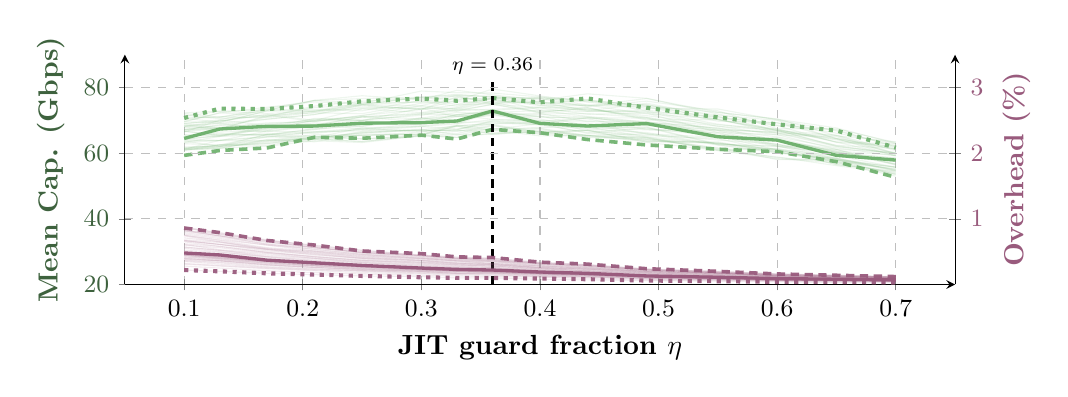
\begin{tikzpicture}
    \begin{axis}[name=ax_main, width=\linewidth, height=4.5cm, xmin=0.05, xmax=0.75, xlabel={JIT guard fraction $\eta$}, axis y line*=left, axis x line=bottom, ymin=20, ymax=90, ylabel={\textcolor{cb_green!55!black}{Mean Cap. (Gbps)}}, ylabel style={font=\bfseries}, ytick={20,40,60,80}, y tick label style={cb_green!55!black}, every axis plot/.append style={mark=none},]
            \addplot[color=cb_green, mark=none, opacity=0.12, line width=0.4pt, solid] coordinates {(0.1,71.24) (0.13,72.74) (0.17,72.1) (0.21,72.68) (0.25,74.92) (0.3,76.98) (0.33,76.11) (0.36,79.53) (0.4,77.45) (0.44,75.56) (0.49,73.65) (0.55,73.46) (0.6,70.12) (0.65,66.79) (0.7,62.19)};
            \addplot[color=cb_green, mark=none, opacity=0.12, line width=0.4pt, solid] coordinates {(0.1,70.71) (0.13,70.93) (0.17,73.64) (0.21,76.04) (0.25,76.63) (0.3,77.07) (0.33,77.92) (0.36,77.07) (0.4,76.64) (0.44,74.19) (0.49,75.85) (0.55,72.89) (0.6,67.45) (0.65,67.42) (0.7,63.23)};
            \addplot[color=cb_green, mark=none, opacity=0.12, line width=0.4pt, solid] coordinates {(0.1,72.06) (0.13,70.95) (0.17,73.06) (0.21,76.06) (0.25,75.17) (0.3,78.93) (0.33,78.43) (0.36,78.31) (0.4,77.14) (0.44,76.06) (0.49,74.48) (0.55,72.4) (0.6,70.33) (0.65,67.69) (0.7,62.96)};
            \addplot[color=cb_green, mark=none, opacity=0.12, line width=0.4pt, solid] coordinates {(0.1,69.73) (0.13,72.22) (0.17,74.0) (0.21,75.62) (0.25,74.85) (0.3,77.1) (0.33,77.69) (0.36,77.21) (0.4,75.52) (0.44,74.39) (0.49,76.66) (0.55,72.46) (0.6,70.43) (0.65,65.3) (0.7,63.46)};
            \addplot[color=cb_green, mark=none, opacity=0.12, line width=0.4pt, solid] coordinates {(0.1,71.6) (0.13,70.52) (0.17,71.18) (0.21,74.35) (0.25,75.82) (0.3,76.69) (0.33,77.41) (0.36,77.37) (0.4,76.63) (0.44,75.74) (0.49,74.67) (0.55,71.57) (0.6,69.97) (0.65,64.45) (0.7,61.72)};
            \addplot[color=cb_green, mark=none, opacity=0.12, line width=0.4pt, solid] coordinates {(0.1,69.56) (0.13,69.31) (0.17,72.92) (0.21,73.36) (0.25,72.9) (0.3,76.1) (0.33,74.91) (0.36,76.82) (0.4,76.81) (0.44,76.29) (0.49,74.2) (0.55,70.77) (0.6,69.19) (0.65,66.09) (0.7,62.9)};
            \addplot[color=cb_green, mark=none, opacity=0.12, line width=0.4pt, solid] coordinates {(0.1,68.39) (0.13,69.09) (0.17,70.37) (0.21,71.75) (0.25,74.71) (0.3,75.75) (0.33,74.28) (0.36,76.88) (0.4,74.62) (0.44,72.76) (0.49,72.57) (0.55,71.15) (0.6,66.92) (0.65,65.49) (0.7,60.82)};
            \addplot[color=cb_green, mark=none, opacity=0.12, line width=0.4pt, solid] coordinates {(0.1,69.04) (0.13,70.15) (0.17,73.36) (0.21,72.91) (0.25,75.33) (0.3,75.48) (0.33,77.57) (0.36,74.96) (0.4,77.12) (0.44,74.69) (0.49,74.84) (0.55,70.25) (0.6,67.26) (0.65,63.46) (0.7,62.76)};
            \addplot[color=cb_green, mark=none, opacity=0.12, line width=0.4pt, solid] coordinates {(0.1,67.25) (0.13,68.44) (0.17,70.34) (0.21,71.82) (0.25,73.98) (0.3,73.52) (0.33,73.7) (0.36,75.9) (0.4,75.18) (0.44,73.17) (0.49,72.51) (0.55,68.15) (0.6,67.04) (0.65,62.05) (0.7,59.77)};
            \addplot[color=cb_green, mark=none, opacity=0.12, line width=0.4pt, solid] coordinates {(0.1,70.58) (0.13,69.5) (0.17,72.83) (0.21,72.76) (0.25,74.73) (0.3,73.4) (0.33,76.1) (0.36,76.89) (0.4,75.06) (0.44,76.2) (0.49,72.85) (0.55,68.83) (0.6,66.72) (0.65,64.31) (0.7,59.99)};
            \addplot[color=cb_green, mark=none, opacity=0.12, line width=0.4pt, solid] coordinates {(0.1,69.5) (0.13,72.32) (0.17,71.23) (0.21,73.92) (0.25,74.71) (0.3,74.49) (0.33,76.9) (0.36,76.28) (0.4,74.51) (0.44,74.52) (0.49,74.08) (0.55,69.74) (0.6,69.29) (0.65,64.49) (0.7,61.24)};
            \addplot[color=cb_green, mark=none, opacity=0.12, line width=0.4pt, solid] coordinates {(0.1,72.26) (0.13,72.82) (0.17,73.11) (0.21,76.1) (0.25,77.5) (0.3,76.25) (0.33,79.15) (0.36,77.77) (0.4,76.14) (0.44,78.08) (0.49,76.71) (0.55,71.91) (0.6,68.52) (0.65,67.12) (0.7,61.89)};
            \addplot[color=cb_green, mark=none, opacity=0.12, line width=0.4pt, solid] coordinates {(0.1,70.59) (0.13,71.1) (0.17,70.8) (0.21,72.42) (0.25,74.42) (0.3,73.33) (0.33,77.21) (0.36,75.56) (0.4,75.67) (0.44,72.9) (0.49,75.2) (0.55,71.14) (0.6,68.37) (0.65,63.26) (0.7,62.17)};
            \addplot[color=cb_green, mark=none, opacity=0.12, line width=0.4pt, solid] coordinates {(0.1,68.96) (0.13,69.83) (0.17,71.61) (0.21,72.27) (0.25,72.04) (0.3,75.22) (0.33,75.7) (0.36,75.16) (0.4,75.58) (0.44,74.62) (0.49,72.0) (0.55,70.41) (0.6,66.11) (0.65,65.39) (0.7,59.91)};
            \addplot[color=cb_green, mark=none, opacity=0.12, line width=0.4pt, solid] coordinates {(0.1,68.88) (0.13,67.8) (0.17,68.94) (0.21,69.79) (0.25,71.04) (0.3,72.19) (0.33,73.12) (0.36,74.78) (0.4,72.66) (0.44,73.57) (0.49,70.93) (0.55,67.32) (0.6,66.24) (0.65,62.37) (0.7,61.44)};
            \addplot[color=cb_green, mark=none, opacity=0.12, line width=0.4pt, solid] coordinates {(0.1,67.75) (0.13,67.6) (0.17,71.1) (0.21,72.86) (0.25,73.55) (0.3,74.13) (0.33,72.91) (0.36,73.38) (0.4,74.02) (0.44,73.86) (0.49,70.44) (0.55,68.27) (0.6,65.55) (0.65,65.03) (0.7,59.69)};
            \addplot[color=cb_green, mark=none, opacity=0.12, line width=0.4pt, solid] coordinates {(0.1,68.09) (0.13,67.81) (0.17,69.23) (0.21,69.63) (0.25,71.45) (0.3,74.48) (0.33,73.38) (0.36,75.67) (0.4,72.35) (0.44,73.85) (0.49,70.11) (0.55,70.2) (0.6,66.86) (0.65,62.32) (0.7,59.77)};
            \addplot[color=cb_green, mark=none, opacity=0.12, line width=0.4pt, solid] coordinates {(0.1,68.14) (0.13,69.77) (0.17,71.86) (0.21,69.97) (0.25,73.5) (0.3,72.37) (0.33,73.87) (0.36,76.67) (0.4,73.16) (0.44,72.65) (0.49,73.16) (0.55,70.17) (0.6,66.96) (0.65,64.44) (0.7,59.16)};
            \addplot[color=cb_green, mark=none, opacity=0.12, line width=0.4pt, solid] coordinates {(0.1,68.48) (0.13,67.27) (0.17,71.51) (0.21,69.65) (0.25,71.49) (0.3,73.28) (0.33,74.76) (0.36,75.01) (0.4,72.24) (0.44,72.05) (0.49,70.82) (0.55,66.97) (0.6,66.54) (0.65,64.06) (0.7,61.27)};
            \addplot[color=cb_green, mark=none, opacity=0.12, line width=0.4pt, solid] coordinates {(0.1,66.4) (0.13,70.07) (0.17,68.45) (0.21,70.38) (0.25,69.99) (0.3,71.91) (0.33,72.79) (0.36,74.93) (0.4,73.89) (0.44,73.28) (0.49,71.43) (0.55,68.64) (0.6,67.35) (0.65,63.38) (0.7,59.23)};
            \addplot[color=cb_green, mark=none, opacity=0.12, line width=0.4pt, solid] coordinates {(0.1,67.1) (0.13,68.67) (0.17,67.75) (0.21,70.6) (0.25,70.06) (0.3,71.54) (0.33,73.43) (0.36,73.05) (0.4,73.79) (0.44,71.85) (0.49,72.21) (0.55,66.28) (0.6,65.64) (0.65,61.19) (0.7,60.18)};
            \addplot[color=cb_green, mark=none, opacity=0.12, line width=0.4pt, solid] coordinates {(0.1,68.12) (0.13,69.16) (0.17,67.59) (0.21,69.92) (0.25,69.95) (0.3,73.7) (0.33,71.06) (0.36,72.37) (0.4,72.99) (0.44,71.21) (0.49,69.47) (0.55,67.56) (0.6,66.07) (0.65,62.02) (0.7,60.13)};
            \addplot[color=cb_green, mark=none, opacity=0.12, line width=0.4pt, solid] coordinates {(0.1,65.58) (0.13,65.44) (0.17,67.83) (0.21,69.24) (0.25,68.23) (0.3,70.43) (0.33,71.62) (0.36,70.29) (0.4,69.73) (0.44,70.66) (0.49,69.57) (0.55,65.86) (0.6,63.96) (0.65,60.19) (0.7,58.53)};
            \addplot[color=cb_green, mark=none, opacity=0.12, line width=0.4pt, solid] coordinates {(0.1,66.66) (0.13,65.68) (0.17,65.76) (0.21,67.18) (0.25,68.86) (0.3,70.34) (0.33,71.22) (0.36,71.37) (0.4,71.13) (0.44,70.44) (0.49,67.24) (0.55,66.79) (0.6,62.5) (0.65,60.08) (0.7,58.49)};
            \addplot[color=cb_green, mark=none, opacity=0.12, line width=0.4pt, solid] coordinates {(0.1,66.67) (0.13,65.41) (0.17,67.3) (0.21,68.77) (0.25,67.41) (0.3,68.92) (0.33,69.49) (0.36,72.21) (0.4,71.32) (0.44,68.28) (0.49,68.91) (0.55,64.87) (0.6,64.72) (0.65,60.2) (0.7,57.38)};
            \addplot[color=cb_green, mark=none, opacity=0.12, line width=0.4pt, solid] coordinates {(0.1,66.65) (0.13,67.4) (0.17,66.48) (0.21,68.38) (0.25,71.06) (0.3,71.9) (0.33,71.7) (0.36,73.03) (0.4,70.98) (0.44,70.81) (0.49,70.7) (0.55,65.26) (0.6,63.9) (0.65,61.15) (0.7,56.7)};
            \addplot[color=cb_green, mark=none, opacity=0.12, line width=0.4pt, solid] coordinates {(0.1,67.11) (0.13,67.76) (0.17,67.71) (0.21,68.66) (0.25,71.0) (0.3,69.52) (0.33,71.61) (0.36,72.84) (0.4,69.79) (0.44,69.81) (0.49,69.43) (0.55,67.7) (0.6,63.88) (0.65,60.66) (0.7,59.36)};
            \addplot[color=cb_green, mark=none, opacity=0.12, line width=0.4pt, solid] coordinates {(0.1,67.01) (0.13,67.47) (0.17,66.96) (0.21,70.19) (0.25,71.13) (0.3,70.46) (0.33,69.99) (0.36,71.66) (0.4,71.78) (0.44,71.04) (0.49,68.35) (0.55,67.07) (0.6,64.98) (0.65,61.63) (0.7,59.2)};
            \addplot[color=cb_green, mark=none, opacity=0.12, line width=0.4pt, solid] coordinates {(0.1,65.55) (0.13,65.07) (0.17,67.6) (0.21,67.33) (0.25,68.4) (0.3,70.65) (0.33,72.42) (0.36,71.92) (0.4,72.11) (0.44,69.61) (0.49,69.15) (0.55,65.27) (0.6,62.09) (0.65,60.04) (0.7,57.41)};
            \addplot[color=cb_green, mark=none, opacity=0.12, line width=0.4pt, solid] coordinates {(0.1,65.18) (0.13,66.44) (0.17,66.74) (0.21,68.71) (0.25,69.93) (0.3,69.13) (0.33,71.77) (0.36,72.31) (0.4,70.4) (0.44,67.78) (0.49,67.1) (0.55,66.25) (0.6,62.21) (0.65,61.09) (0.7,56.35)};
            \addplot[color=cb_green, mark=none, opacity=0.12, line width=0.4pt, solid] coordinates {(0.1,64.33) (0.13,65.14) (0.17,68.23) (0.21,68.6) (0.25,68.14) (0.3,70.84) (0.33,68.97) (0.36,72.41) (0.4,69.0) (0.44,70.79) (0.49,69.21) (0.55,66.97) (0.6,63.99) (0.65,60.59) (0.7,56.64)};
            \addplot[color=cb_green, mark=none, opacity=0.12, line width=0.4pt, solid] coordinates {(0.1,65.01) (0.13,66.0) (0.17,65.43) (0.21,67.53) (0.25,69.31) (0.3,68.57) (0.33,71.21) (0.36,71.95) (0.4,68.75) (0.44,68.7) (0.49,65.78) (0.55,64.02) (0.6,62.7) (0.65,60.38) (0.7,57.62)};
            \addplot[color=cb_green, mark=none, opacity=0.12, line width=0.4pt, solid] coordinates {(0.1,64.2) (0.13,65.39) (0.17,65.83) (0.21,66.48) (0.25,67.71) (0.3,68.1) (0.33,68.95) (0.36,70.2) (0.4,69.96) (0.44,66.82) (0.49,65.36) (0.55,64.46) (0.6,60.45) (0.65,57.72) (0.7,55.78)};
            \addplot[color=cb_green, mark=none, opacity=0.12, line width=0.4pt, solid] coordinates {(0.1,61.5) (0.13,62.55) (0.17,64.03) (0.21,63.47) (0.25,65.79) (0.3,65.76) (0.33,66.64) (0.36,68.55) (0.4,65.84) (0.44,65.0) (0.49,64.51) (0.55,61.18) (0.6,61.47) (0.65,57.82) (0.7,55.06)};
            \addplot[color=cb_green, mark=none, opacity=0.12, line width=0.4pt, solid] coordinates {(0.1,61.35) (0.13,62.49) (0.17,62.88) (0.21,65.05) (0.25,64.39) (0.3,65.11) (0.33,65.61) (0.36,65.84) (0.4,66.47) (0.44,65.34) (0.49,64.68) (0.55,60.81) (0.6,58.85) (0.65,56.2) (0.7,53.72)};
            \addplot[color=cb_green, mark=none, opacity=0.12, line width=0.4pt, solid] coordinates {(0.1,60.97) (0.13,61.41) (0.17,64.15) (0.21,64.26) (0.25,66.61) (0.3,67.12) (0.33,68.29) (0.36,65.66) (0.4,67.03) (0.44,65.45) (0.49,65.89) (0.55,62.45) (0.6,60.06) (0.65,58.35) (0.7,54.69)};
            \addplot[color=cb_green, mark=none, opacity=0.12, line width=0.4pt, solid] coordinates {(0.1,61.18) (0.13,63.93) (0.17,65.11) (0.21,64.14) (0.25,65.48) (0.3,65.69) (0.33,68.42) (0.36,68.77) (0.4,66.41) (0.44,66.98) (0.49,64.75) (0.55,61.01) (0.6,61.22) (0.65,56.47) (0.7,54.52)};
            \addplot[color=cb_green, mark=none, opacity=0.12, line width=0.4pt, solid] coordinates {(0.1,63.67) (0.13,62.13) (0.17,65.72) (0.21,65.2) (0.25,64.3) (0.3,65.54) (0.33,68.21) (0.36,69.21) (0.4,68.65) (0.44,66.32) (0.49,64.2) (0.55,63.1) (0.6,61.17) (0.65,59.23) (0.7,55.72)};
            \addplot[color=cb_green, mark=none, opacity=0.12, line width=0.4pt, solid] coordinates {(0.1,63.24) (0.13,65.09) (0.17,65.58) (0.21,64.47) (0.25,66.33) (0.3,66.97) (0.33,66.78) (0.36,67.3) (0.4,68.97) (0.44,67.31) (0.49,66.28) (0.55,62.64) (0.6,60.31) (0.65,58.0) (0.7,55.77)};
            \addplot[color=cb_green, mark=none, opacity=0.12, line width=0.4pt, solid] coordinates {(0.1,62.9) (0.13,62.47) (0.17,65.67) (0.21,66.06) (0.25,67.28) (0.3,68.29) (0.33,69.42) (0.36,69.48) (0.4,69.01) (0.44,66.02) (0.49,67.8) (0.55,62.57) (0.6,62.24) (0.65,58.04) (0.7,54.55)};
            \addplot[color=cb_green, mark=none, opacity=0.12, line width=0.4pt, solid] coordinates {(0.1,64.03) (0.13,63.91) (0.17,64.86) (0.21,66.56) (0.25,66.81) (0.3,68.1) (0.33,67.38) (0.36,68.9) (0.4,69.43) (0.44,67.7) (0.49,68.0) (0.55,62.78) (0.6,61.99) (0.65,59.92) (0.7,56.6)};
            \addplot[color=cb_green, mark=none, opacity=0.12, line width=0.4pt, solid] coordinates {(0.1,64.02) (0.13,63.81) (0.17,66.77) (0.21,66.32) (0.25,67.2) (0.3,66.81) (0.33,67.04) (0.36,69.73) (0.4,68.66) (0.44,69.17) (0.49,65.93) (0.55,64.82) (0.6,62.79) (0.65,58.34) (0.7,55.62)};
            \addplot[color=cb_green, mark=none, opacity=0.12, line width=0.4pt, solid] coordinates {(0.1,63.33) (0.13,63.82) (0.17,63.76) (0.21,64.77) (0.25,67.67) (0.3,66.6) (0.33,67.19) (0.36,69.95) (0.4,69.26) (0.44,68.38) (0.49,67.55) (0.55,65.15) (0.6,61.01) (0.65,58.55) (0.7,54.9)};
            \addplot[color=cb_green, mark=none, opacity=0.12, line width=0.4pt, solid] coordinates {(0.1,60.99) (0.13,61.97) (0.17,65.04) (0.21,65.1) (0.25,65.44) (0.3,65.82) (0.33,68.23) (0.36,66.98) (0.4,67.89) (0.44,67.97) (0.49,64.97) (0.55,62.9) (0.6,60.97) (0.65,57.35) (0.7,55.25)};
            \addplot[color=cb_green, mark=none, opacity=0.12, line width=0.4pt, solid] coordinates {(0.1,61.8) (0.13,62.07) (0.17,62.97) (0.21,64.14) (0.25,63.6) (0.3,65.43) (0.33,65.97) (0.36,68.35) (0.4,66.48) (0.44,66.97) (0.49,63.61) (0.55,63.03) (0.6,61.03) (0.65,57.12) (0.7,53.98)};
            \addplot[color=cb_green, mark=none, opacity=0.12, line width=0.4pt, solid] coordinates {(0.1,60.87) (0.13,62.52) (0.17,62.39) (0.21,64.57) (0.25,66.19) (0.3,67.31) (0.33,65.56) (0.36,67.52) (0.4,65.76) (0.44,66.97) (0.49,63.28) (0.55,60.85) (0.6,58.33) (0.65,57.12) (0.7,52.98)};
            \addplot[color=cb_green, mark=none, opacity=0.12, line width=0.4pt, solid] coordinates {(0.1,61.82) (0.13,62.17) (0.17,63.81) (0.21,65.65) (0.25,65.35) (0.3,66.38) (0.33,68.54) (0.36,67.41) (0.4,67.58) (0.44,65.37) (0.49,63.86) (0.55,63.12) (0.6,60.57) (0.65,56.6) (0.7,54.25)};
            \addplot[color=cb_green, mark=none, opacity=0.12, line width=0.4pt, solid] coordinates {(0.1,61.38) (0.13,61.92) (0.17,63.3) (0.21,64.63) (0.25,66.08) (0.3,67.01) (0.33,67.01) (0.36,66.14) (0.4,66.47) (0.44,65.4) (0.49,63.49) (0.55,63.44) (0.6,60.13) (0.65,58.33) (0.7,54.79)};
            \addplot[color=cb_green, mark=none, opacity=0.12, line width=0.4pt, solid] coordinates {(0.1,61.02) (0.13,61.52) (0.17,62.12) (0.21,63.78) (0.25,63.24) (0.3,65.27) (0.33,64.81) (0.36,65.97) (0.4,67.47) (0.44,64.83) (0.49,64.14) (0.55,61.63) (0.6,58.04) (0.65,58.1) (0.7,53.43)};
            \addplot[color=cb_green, mark=none, opacity=0.12, line width=0.4pt, solid] coordinates {(0.1,61.29) (0.13,61.62) (0.17,63.63) (0.21,64.46) (0.25,63.47) (0.3,65.42) (0.33,64.82) (0.36,67.03) (0.4,65.25) (0.44,65.35) (0.49,64.89) (0.55,61.42) (0.6,58.63) (0.65,57.51) (0.7,53.6)};
            \addplot[color=cb_green, mark=none, dotted, line width=1.5pt, opacity=0.95] coordinates {(0.1,70.7) (0.13,73.58) (0.17,73.44) (0.21,74.36) (0.25,75.8) (0.3,76.63) (0.33,75.96) (0.36,76.78) (0.4,75.48) (0.44,76.68) (0.49,73.83) (0.55,70.91) (0.6,68.78) (0.65,66.89) (0.7,61.66)};
            \addplot[color=cb_green, mark=none, solid, very thick] coordinates {(0.1,64.49) (0.13,67.35) (0.17,68.19) (0.21,68.25) (0.25,69.13) (0.3,69.31) (0.33,69.79) (0.36,72.86) (0.4,69.08) (0.44,68.28) (0.49,69.01) (0.55,65.0) (0.6,63.97) (0.65,59.33) (0.7,57.9)};
            \addplot[color=cb_green, mark=none, densely dashed, line width=1.3pt, opacity=0.95] coordinates {(0.1,59.33) (0.13,60.81) (0.17,61.6) (0.21,64.85) (0.25,64.55) (0.3,65.48) (0.33,64.31) (0.36,67.25) (0.4,66.22) (0.44,64.16) (0.49,62.5) (0.55,61.21) (0.6,60.45) (0.65,57.4) (0.7,52.67)};
            \draw[densely dashed, black, line width=0.8pt] (axis cs:0.36, 20) -- (axis cs:0.36, 90);
            \node[anchor=south, font=\scriptsize, fill=white, inner sep=1pt] at (axis cs:0.36, 83) {$\eta=0.36$};
    \end{axis}
    \begin{axis}[at={(ax_main.south west)}, anchor=south west, width=\linewidth, height=4.5cm, xmin=0.05, xmax=0.75, axis y line*=right, axis x line=none, ymin=0, ymax=3.5, ytick={1,2,3}, ylabel={\textcolor{cb_reddish_purple!75!black}{Overhead (\%)}}, ylabel style={font=\bfseries}, y tick label style={cb_reddish_purple!75!black}, every axis plot/.append style={mark=none},]
        \addplot[color=cb_reddish_purple!75!black, mark=none, opacity=0.12, line width=0.4pt, solid] coordinates {(0.1,0.22) (0.13,0.2) (0.17,0.17) (0.21,0.15) (0.25,0.13) (0.3,0.12) (0.33,0.1) (0.36,0.1) (0.4,0.08) (0.44,0.07) (0.49,0.06) (0.55,0.05) (0.6,0.04) (0.65,0.03) (0.7,0.03)};
        \addplot[color=cb_reddish_purple!75!black, mark=none, opacity=0.12, line width=0.4pt, solid] coordinates {(0.1,0.28) (0.13,0.25) (0.17,0.21) (0.21,0.18) (0.25,0.16) (0.3,0.14) (0.33,0.13) (0.36,0.12) (0.4,0.11) (0.44,0.09) (0.49,0.07) (0.55,0.06) (0.6,0.05) (0.65,0.04) (0.7,0.04)};
        \addplot[color=cb_reddish_purple!75!black, mark=none, opacity=0.12, line width=0.4pt, solid] coordinates {(0.1,0.31) (0.13,0.28) (0.17,0.24) (0.21,0.21) (0.25,0.18) (0.3,0.16) (0.33,0.15) (0.36,0.14) (0.4,0.12) (0.44,0.11) (0.49,0.08) (0.55,0.07) (0.6,0.06) (0.65,0.05) (0.7,0.04)};
        \addplot[color=cb_reddish_purple!75!black, mark=none, opacity=0.12, line width=0.4pt, solid] coordinates {(0.1,0.32) (0.13,0.29) (0.17,0.25) (0.21,0.22) (0.25,0.2) (0.3,0.17) (0.33,0.16) (0.36,0.15) (0.4,0.12) (0.44,0.11) (0.49,0.09) (0.55,0.07) (0.6,0.06) (0.65,0.05) (0.7,0.05)};
        \addplot[color=cb_reddish_purple!75!black, mark=none, opacity=0.12, line width=0.4pt, solid] coordinates {(0.1,0.35) (0.13,0.31) (0.17,0.26) (0.21,0.23) (0.25,0.21) (0.3,0.18) (0.33,0.17) (0.36,0.16) (0.4,0.13) (0.44,0.12) (0.49,0.09) (0.55,0.08) (0.6,0.06) (0.65,0.06) (0.7,0.05)};
        \addplot[color=cb_reddish_purple!75!black, mark=none, opacity=0.12, line width=0.4pt, solid] coordinates {(0.1,0.36) (0.13,0.33) (0.17,0.27) (0.21,0.24) (0.25,0.21) (0.3,0.19) (0.33,0.17) (0.36,0.17) (0.4,0.14) (0.44,0.12) (0.49,0.1) (0.55,0.08) (0.6,0.06) (0.65,0.06) (0.7,0.05)};
        \addplot[color=cb_reddish_purple!75!black, mark=none, opacity=0.12, line width=0.4pt, solid] coordinates {(0.1,0.37) (0.13,0.34) (0.17,0.29) (0.21,0.26) (0.25,0.22) (0.3,0.2) (0.33,0.17) (0.36,0.17) (0.4,0.14) (0.44,0.13) (0.49,0.1) (0.55,0.08) (0.6,0.07) (0.65,0.06) (0.7,0.05)};
        \addplot[color=cb_reddish_purple!75!black, mark=none, opacity=0.12, line width=0.4pt, solid] coordinates {(0.1,0.38) (0.13,0.36) (0.17,0.3) (0.21,0.26) (0.25,0.23) (0.3,0.2) (0.33,0.19) (0.36,0.18) (0.4,0.15) (0.44,0.13) (0.49,0.1) (0.55,0.09) (0.6,0.07) (0.65,0.06) (0.7,0.05)};
        \addplot[color=cb_reddish_purple!75!black, mark=none, opacity=0.12, line width=0.4pt, solid] coordinates {(0.1,0.4) (0.13,0.36) (0.17,0.3) (0.21,0.26) (0.25,0.23) (0.3,0.2) (0.33,0.18) (0.36,0.18) (0.4,0.16) (0.44,0.14) (0.49,0.11) (0.55,0.09) (0.6,0.07) (0.65,0.06) (0.7,0.05)};
        \addplot[color=cb_reddish_purple!75!black, mark=none, opacity=0.12, line width=0.4pt, solid] coordinates {(0.1,0.39) (0.13,0.36) (0.17,0.31) (0.21,0.28) (0.25,0.24) (0.3,0.21) (0.33,0.2) (0.36,0.18) (0.4,0.16) (0.44,0.14) (0.49,0.11) (0.55,0.09) (0.6,0.07) (0.65,0.06) (0.7,0.05)};
        \addplot[color=cb_reddish_purple!75!black, mark=none, opacity=0.12, line width=0.4pt, solid] coordinates {(0.1,0.4) (0.13,0.37) (0.17,0.33) (0.21,0.29) (0.25,0.25) (0.3,0.22) (0.33,0.2) (0.36,0.19) (0.4,0.16) (0.44,0.14) (0.49,0.11) (0.55,0.09) (0.6,0.08) (0.65,0.07) (0.7,0.06)};
        \addplot[color=cb_reddish_purple!75!black, mark=none, opacity=0.12, line width=0.4pt, solid] coordinates {(0.1,0.42) (0.13,0.38) (0.17,0.32) (0.21,0.28) (0.25,0.24) (0.3,0.22) (0.33,0.21) (0.36,0.19) (0.4,0.16) (0.44,0.14) (0.49,0.12) (0.55,0.1) (0.6,0.07) (0.65,0.07) (0.7,0.06)};
        \addplot[color=cb_reddish_purple!75!black, mark=none, opacity=0.12, line width=0.4pt, solid] coordinates {(0.1,0.42) (0.13,0.39) (0.17,0.34) (0.21,0.29) (0.25,0.26) (0.3,0.22) (0.33,0.2) (0.36,0.2) (0.4,0.16) (0.44,0.15) (0.49,0.12) (0.55,0.1) (0.6,0.08) (0.65,0.07) (0.7,0.06)};
        \addplot[color=cb_reddish_purple!75!black, mark=none, opacity=0.12, line width=0.4pt, solid] coordinates {(0.1,0.44) (0.13,0.39) (0.17,0.33) (0.21,0.29) (0.25,0.26) (0.3,0.22) (0.33,0.2) (0.36,0.2) (0.4,0.17) (0.44,0.15) (0.49,0.12) (0.55,0.1) (0.6,0.08) (0.65,0.07) (0.7,0.06)};
        \addplot[color=cb_reddish_purple!75!black, mark=none, opacity=0.12, line width=0.4pt, solid] coordinates {(0.1,0.44) (0.13,0.4) (0.17,0.35) (0.21,0.31) (0.25,0.27) (0.3,0.23) (0.33,0.22) (0.36,0.2) (0.4,0.17) (0.44,0.15) (0.49,0.12) (0.55,0.1) (0.6,0.08) (0.65,0.07) (0.7,0.06)};
        \addplot[color=cb_reddish_purple!75!black, mark=none, opacity=0.12, line width=0.4pt, solid] coordinates {(0.1,0.45) (0.13,0.4) (0.17,0.35) (0.21,0.3) (0.25,0.27) (0.3,0.24) (0.33,0.21) (0.36,0.21) (0.4,0.17) (0.44,0.15) (0.49,0.12) (0.55,0.1) (0.6,0.08) (0.65,0.07) (0.7,0.06)};
        \addplot[color=cb_reddish_purple!75!black, mark=none, opacity=0.12, line width=0.4pt, solid] coordinates {(0.1,0.45) (0.13,0.41) (0.17,0.35) (0.21,0.31) (0.25,0.27) (0.3,0.23) (0.33,0.22) (0.36,0.2) (0.4,0.18) (0.44,0.15) (0.49,0.12) (0.55,0.1) (0.6,0.08) (0.65,0.07) (0.7,0.06)};
        \addplot[color=cb_reddish_purple!75!black, mark=none, opacity=0.12, line width=0.4pt, solid] coordinates {(0.1,0.45) (0.13,0.41) (0.17,0.35) (0.21,0.31) (0.25,0.27) (0.3,0.25) (0.33,0.21) (0.36,0.21) (0.4,0.17) (0.44,0.16) (0.49,0.13) (0.55,0.11) (0.6,0.08) (0.65,0.07) (0.7,0.06)};
        \addplot[color=cb_reddish_purple!75!black, mark=none, opacity=0.12, line width=0.4pt, solid] coordinates {(0.1,0.46) (0.13,0.42) (0.17,0.36) (0.21,0.31) (0.25,0.28) (0.3,0.24) (0.33,0.22) (0.36,0.21) (0.4,0.18) (0.44,0.16) (0.49,0.13) (0.55,0.1) (0.6,0.08) (0.65,0.08) (0.7,0.06)};
        \addplot[color=cb_reddish_purple!75!black, mark=none, opacity=0.12, line width=0.4pt, solid] coordinates {(0.1,0.46) (0.13,0.42) (0.17,0.37) (0.21,0.33) (0.25,0.27) (0.3,0.25) (0.33,0.23) (0.36,0.21) (0.4,0.18) (0.44,0.16) (0.49,0.13) (0.55,0.11) (0.6,0.09) (0.65,0.08) (0.7,0.06)};
        \addplot[color=cb_reddish_purple!75!black, mark=none, opacity=0.12, line width=0.4pt, solid] coordinates {(0.1,0.47) (0.13,0.43) (0.17,0.36) (0.21,0.32) (0.25,0.28) (0.3,0.25) (0.33,0.23) (0.36,0.22) (0.4,0.19) (0.44,0.16) (0.49,0.13) (0.55,0.11) (0.6,0.09) (0.65,0.07) (0.7,0.06)};
        \addplot[color=cb_reddish_purple!75!black, mark=none, opacity=0.12, line width=0.4pt, solid] coordinates {(0.1,0.48) (0.13,0.43) (0.17,0.37) (0.21,0.33) (0.25,0.28) (0.3,0.25) (0.33,0.23) (0.36,0.22) (0.4,0.18) (0.44,0.16) (0.49,0.13) (0.55,0.11) (0.6,0.09) (0.65,0.08) (0.7,0.06)};
        \addplot[color=cb_reddish_purple!75!black, mark=none, opacity=0.12, line width=0.4pt, solid] coordinates {(0.1,0.47) (0.13,0.43) (0.17,0.36) (0.21,0.33) (0.25,0.29) (0.3,0.25) (0.33,0.23) (0.36,0.22) (0.4,0.18) (0.44,0.16) (0.49,0.13) (0.55,0.11) (0.6,0.09) (0.65,0.08) (0.7,0.06)};
        \addplot[color=cb_reddish_purple!75!black, mark=none, opacity=0.12, line width=0.4pt, solid] coordinates {(0.1,0.49) (0.13,0.45) (0.17,0.37) (0.21,0.34) (0.25,0.28) (0.3,0.26) (0.33,0.24) (0.36,0.22) (0.4,0.19) (0.44,0.17) (0.49,0.13) (0.55,0.11) (0.6,0.09) (0.65,0.08) (0.7,0.07)};
        \addplot[color=cb_reddish_purple!75!black, mark=none, opacity=0.12, line width=0.4pt, solid] coordinates {(0.1,0.5) (0.13,0.47) (0.17,0.4) (0.21,0.35) (0.25,0.3) (0.3,0.27) (0.33,0.25) (0.36,0.23) (0.4,0.2) (0.44,0.17) (0.49,0.14) (0.55,0.12) (0.6,0.09) (0.65,0.08) (0.7,0.07)};
        \addplot[color=cb_reddish_purple!75!black, mark=none, opacity=0.12, line width=0.4pt, solid] coordinates {(0.1,0.52) (0.13,0.49) (0.17,0.42) (0.21,0.36) (0.25,0.31) (0.3,0.27) (0.33,0.26) (0.36,0.25) (0.4,0.2) (0.44,0.18) (0.49,0.14) (0.55,0.12) (0.6,0.1) (0.65,0.08) (0.7,0.07)};
        \addplot[color=cb_reddish_purple!75!black, mark=none, opacity=0.12, line width=0.4pt, solid] coordinates {(0.1,0.55) (0.13,0.5) (0.17,0.42) (0.21,0.37) (0.25,0.33) (0.3,0.28) (0.33,0.26) (0.36,0.25) (0.4,0.21) (0.44,0.18) (0.49,0.15) (0.55,0.13) (0.6,0.1) (0.65,0.09) (0.7,0.07)};
        \addplot[color=cb_reddish_purple!75!black, mark=none, opacity=0.12, line width=0.4pt, solid] coordinates {(0.1,0.57) (0.13,0.52) (0.17,0.43) (0.21,0.39) (0.25,0.33) (0.3,0.29) (0.33,0.27) (0.36,0.26) (0.4,0.22) (0.44,0.19) (0.49,0.15) (0.55,0.13) (0.6,0.1) (0.65,0.09) (0.7,0.08)};
        \addplot[color=cb_reddish_purple!75!black, mark=none, opacity=0.12, line width=0.4pt, solid] coordinates {(0.1,0.57) (0.13,0.52) (0.17,0.45) (0.21,0.4) (0.25,0.34) (0.3,0.3) (0.33,0.28) (0.36,0.26) (0.4,0.22) (0.44,0.2) (0.49,0.16) (0.55,0.13) (0.6,0.11) (0.65,0.09) (0.7,0.08)};
        \addplot[color=cb_reddish_purple!75!black, mark=none, opacity=0.12, line width=0.4pt, solid] coordinates {(0.1,0.61) (0.13,0.53) (0.17,0.47) (0.21,0.4) (0.25,0.35) (0.3,0.31) (0.33,0.29) (0.36,0.28) (0.4,0.23) (0.44,0.2) (0.49,0.17) (0.55,0.13) (0.6,0.11) (0.65,0.09) (0.7,0.08)};
        \addplot[color=cb_reddish_purple!75!black, mark=none, opacity=0.12, line width=0.4pt, solid] coordinates {(0.1,0.6) (0.13,0.56) (0.17,0.48) (0.21,0.42) (0.25,0.37) (0.3,0.32) (0.33,0.3) (0.36,0.28) (0.4,0.24) (0.44,0.21) (0.49,0.16) (0.55,0.14) (0.6,0.11) (0.65,0.1) (0.7,0.08)};
        \addplot[color=cb_reddish_purple!75!black, mark=none, opacity=0.12, line width=0.4pt, solid] coordinates {(0.1,0.62) (0.13,0.58) (0.17,0.49) (0.21,0.42) (0.25,0.36) (0.3,0.33) (0.33,0.3) (0.36,0.28) (0.4,0.24) (0.44,0.21) (0.49,0.17) (0.55,0.14) (0.6,0.11) (0.65,0.1) (0.7,0.09)};
        \addplot[color=cb_reddish_purple!75!black, mark=none, opacity=0.12, line width=0.4pt, solid] coordinates {(0.1,0.65) (0.13,0.58) (0.17,0.49) (0.21,0.43) (0.25,0.37) (0.3,0.34) (0.33,0.31) (0.36,0.3) (0.4,0.25) (0.44,0.21) (0.49,0.18) (0.55,0.15) (0.6,0.12) (0.65,0.1) (0.7,0.09)};
        \addplot[color=cb_reddish_purple!75!black, mark=none, opacity=0.12, line width=0.4pt, solid] coordinates {(0.1,0.67) (0.13,0.61) (0.17,0.51) (0.21,0.46) (0.25,0.39) (0.3,0.34) (0.33,0.32) (0.36,0.3) (0.4,0.25) (0.44,0.23) (0.49,0.18) (0.55,0.15) (0.6,0.12) (0.65,0.11) (0.7,0.09)};
        \addplot[color=cb_reddish_purple!75!black, mark=none, opacity=0.12, line width=0.4pt, solid] coordinates {(0.1,0.66) (0.13,0.61) (0.17,0.53) (0.21,0.45) (0.25,0.4) (0.3,0.36) (0.33,0.32) (0.36,0.3) (0.4,0.26) (0.44,0.23) (0.49,0.18) (0.55,0.15) (0.6,0.12) (0.65,0.11) (0.7,0.09)};
        \addplot[color=cb_reddish_purple!75!black, mark=none, opacity=0.12, line width=0.4pt, solid] coordinates {(0.1,0.67) (0.13,0.61) (0.17,0.54) (0.21,0.47) (0.25,0.4) (0.3,0.36) (0.33,0.33) (0.36,0.31) (0.4,0.26) (0.44,0.23) (0.49,0.19) (0.55,0.16) (0.6,0.13) (0.65,0.11) (0.7,0.09)};
        \addplot[color=cb_reddish_purple!75!black, mark=none, opacity=0.12, line width=0.4pt, solid] coordinates {(0.1,0.68) (0.13,0.64) (0.17,0.53) (0.21,0.48) (0.25,0.41) (0.3,0.37) (0.33,0.33) (0.36,0.32) (0.4,0.26) (0.44,0.24) (0.49,0.19) (0.55,0.16) (0.6,0.13) (0.65,0.11) (0.7,0.09)};
        \addplot[color=cb_reddish_purple!75!black, mark=none, opacity=0.12, line width=0.4pt, solid] coordinates {(0.1,0.71) (0.13,0.65) (0.17,0.54) (0.21,0.5) (0.25,0.42) (0.3,0.37) (0.33,0.35) (0.36,0.32) (0.4,0.28) (0.44,0.24) (0.49,0.2) (0.55,0.17) (0.6,0.13) (0.65,0.11) (0.7,0.1)};
        \addplot[color=cb_reddish_purple!75!black, mark=none, opacity=0.12, line width=0.4pt, solid] coordinates {(0.1,0.74) (0.13,0.65) (0.17,0.55) (0.21,0.49) (0.25,0.43) (0.3,0.39) (0.33,0.36) (0.36,0.32) (0.4,0.28) (0.44,0.25) (0.49,0.2) (0.55,0.17) (0.6,0.13) (0.65,0.12) (0.7,0.1)};
        \addplot[color=cb_reddish_purple!75!black, mark=none, opacity=0.12, line width=0.4pt, solid] coordinates {(0.1,0.75) (0.13,0.67) (0.17,0.56) (0.21,0.51) (0.25,0.44) (0.3,0.39) (0.33,0.36) (0.36,0.34) (0.4,0.28) (0.44,0.25) (0.49,0.2) (0.55,0.17) (0.6,0.13) (0.65,0.12) (0.7,0.1)};
        \addplot[color=cb_reddish_purple!75!black, mark=none, opacity=0.12, line width=0.4pt, solid] coordinates {(0.1,0.75) (0.13,0.68) (0.17,0.6) (0.21,0.51) (0.25,0.45) (0.3,0.4) (0.33,0.36) (0.36,0.35) (0.4,0.29) (0.44,0.26) (0.49,0.2) (0.55,0.17) (0.6,0.14) (0.65,0.12) (0.7,0.11)};
        \addplot[color=cb_reddish_purple!75!black, mark=none, opacity=0.12, line width=0.4pt, solid] coordinates {(0.1,0.77) (0.13,0.7) (0.17,0.6) (0.21,0.54) (0.25,0.46) (0.3,0.4) (0.33,0.38) (0.36,0.35) (0.4,0.3) (0.44,0.26) (0.49,0.21) (0.55,0.17) (0.6,0.14) (0.65,0.12) (0.7,0.1)};
        \addplot[color=cb_reddish_purple!75!black, mark=none, opacity=0.12, line width=0.4pt, solid] coordinates {(0.1,0.79) (0.13,0.72) (0.17,0.62) (0.21,0.53) (0.25,0.46) (0.3,0.41) (0.33,0.37) (0.36,0.36) (0.4,0.31) (0.44,0.27) (0.49,0.22) (0.55,0.18) (0.6,0.14) (0.65,0.13) (0.7,0.11)};
        \addplot[color=cb_reddish_purple!75!black, mark=none, opacity=0.12, line width=0.4pt, solid] coordinates {(0.1,0.81) (0.13,0.74) (0.17,0.61) (0.21,0.56) (0.25,0.48) (0.3,0.42) (0.33,0.39) (0.36,0.37) (0.4,0.31) (0.44,0.28) (0.49,0.22) (0.55,0.18) (0.6,0.14) (0.65,0.13) (0.7,0.11)};
        \addplot[color=cb_reddish_purple!75!black, mark=none, opacity=0.12, line width=0.4pt, solid] coordinates {(0.1,0.83) (0.13,0.74) (0.17,0.64) (0.21,0.57) (0.25,0.48) (0.3,0.43) (0.33,0.39) (0.36,0.36) (0.4,0.32) (0.44,0.28) (0.49,0.22) (0.55,0.18) (0.6,0.15) (0.65,0.13) (0.7,0.11)};
        \addplot[color=cb_reddish_purple!75!black, mark=none, opacity=0.12, line width=0.4pt, solid] coordinates {(0.1,0.82) (0.13,0.74) (0.17,0.65) (0.21,0.56) (0.25,0.49) (0.3,0.44) (0.33,0.4) (0.36,0.37) (0.4,0.32) (0.44,0.28) (0.49,0.22) (0.55,0.18) (0.6,0.15) (0.65,0.13) (0.7,0.11)};
        \addplot[color=cb_reddish_purple!75!black, mark=none, opacity=0.12, line width=0.4pt, solid] coordinates {(0.1,0.82) (0.13,0.77) (0.17,0.66) (0.21,0.56) (0.25,0.49) (0.3,0.44) (0.33,0.4) (0.36,0.39) (0.4,0.32) (0.44,0.29) (0.49,0.23) (0.55,0.19) (0.6,0.15) (0.65,0.14) (0.7,0.11)};
        \addplot[color=cb_reddish_purple!75!black, mark=none, opacity=0.12, line width=0.4pt, solid] coordinates {(0.1,0.87) (0.13,0.76) (0.17,0.67) (0.21,0.58) (0.25,0.5) (0.3,0.44) (0.33,0.41) (0.36,0.38) (0.4,0.33) (0.44,0.3) (0.49,0.23) (0.55,0.2) (0.6,0.16) (0.65,0.13) (0.7,0.11)};
        \addplot[color=cb_reddish_purple!75!black, mark=none, opacity=0.12, line width=0.4pt, solid] coordinates {(0.1,0.88) (0.13,0.78) (0.17,0.67) (0.21,0.6) (0.25,0.52) (0.3,0.44) (0.33,0.4) (0.36,0.4) (0.4,0.34) (0.44,0.3) (0.49,0.24) (0.55,0.19) (0.6,0.16) (0.65,0.14) (0.7,0.12)};
        \addplot[color=cb_reddish_purple!75!black, mark=none, opacity=0.12, line width=0.4pt, solid] coordinates {(0.1,0.86) (0.13,0.79) (0.17,0.68) (0.21,0.59) (0.25,0.52) (0.3,0.45) (0.33,0.42) (0.36,0.4) (0.4,0.33) (0.44,0.3) (0.49,0.23) (0.55,0.2) (0.6,0.16) (0.65,0.14) (0.7,0.12)};
        \addplot[color=cb_reddish_purple!75!black, mark=none, dotted, line width=1.5pt, opacity=0.95] coordinates {(0.1,0.22) (0.13,0.2) (0.17,0.17) (0.21,0.15) (0.25,0.13) (0.3,0.11) (0.33,0.1) (0.36,0.1) (0.4,0.09) (0.44,0.08) (0.49,0.06) (0.55,0.05) (0.6,0.04) (0.65,0.04) (0.7,0.03)};
        \addplot[color=cb_reddish_purple!75!black, mark=none, solid, very thick] coordinates {(0.1,0.48) (0.13,0.45) (0.17,0.37) (0.21,0.33) (0.25,0.29) (0.3,0.25) (0.33,0.23) (0.36,0.22) (0.4,0.19) (0.44,0.17) (0.49,0.13) (0.55,0.11) (0.6,0.09) (0.65,0.08) (0.7,0.07)};
        \addplot[color=cb_reddish_purple!75!black, mark=none, densely dashed, line width=1.3pt, opacity=0.95] coordinates {(0.1,0.86) (0.13,0.79) (0.17,0.67) (0.21,0.6) (0.25,0.51) (0.3,0.47) (0.33,0.42) (0.36,0.41) (0.4,0.34) (0.44,0.31) (0.49,0.24) (0.55,0.2) (0.6,0.16) (0.65,0.14) (0.7,0.12)};
    \end{axis}
\end{tikzpicture}
        \vspace{-25pt}
        \caption{Translational}
    \end{subfigure}%
    \hspace{30pt}%
    \begin{subfigure}{0.425\linewidth}
        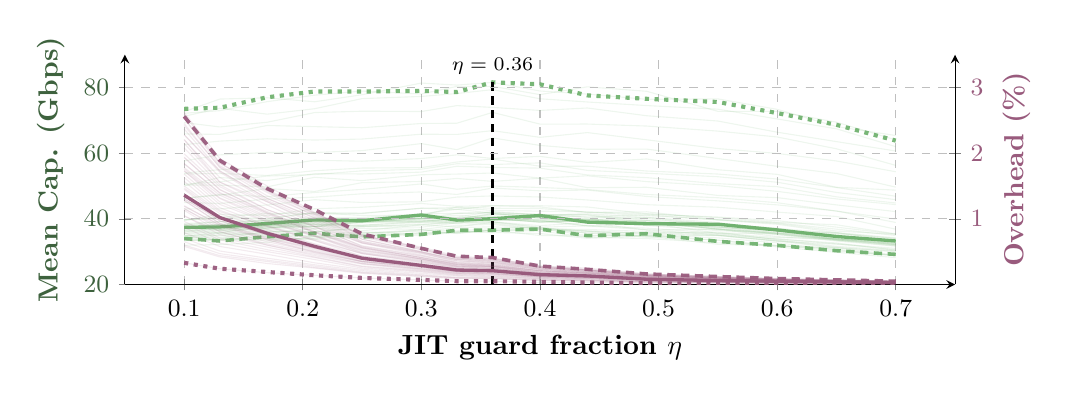
\begin{tikzpicture}
    \begin{axis}[name=ax_main, width=\linewidth, height=4.5cm, xmin=0.05, xmax=0.75, xlabel={JIT guard fraction $\eta$}, axis y line*=left, axis x line=bottom, ymin=20, ymax=90, ylabel={\textcolor{cb_green!55!black}{Mean Cap. (Gbps)}}, ylabel style={font=\bfseries}, ytick={20,40,60,80}, y tick label style={cb_green!55!black}, every axis plot/.append style={mark=none},]
            \addplot[color=cb_green, mark=none, opacity=0.12, line width=0.4pt, solid] coordinates {(0.1,72.64) (0.13,76.48) (0.17,76.87) (0.21,75.66) (0.25,77.8) (0.3,81.36) (0.33,80.74) (0.36,81.56) (0.4,78.94) (0.44,77.99) (0.49,76.4) (0.55,76.53) (0.6,73.35) (0.65,68.09) (0.7,65.38)};
            \addplot[color=cb_green, mark=none, opacity=0.12, line width=0.4pt, solid] coordinates {(0.1,72.15) (0.13,72.94) (0.17,75.7) (0.21,77.66) (0.25,78.92) (0.3,78.02) (0.33,80.34) (0.36,80.37) (0.4,77.83) (0.44,80.21) (0.49,78.85) (0.55,72.74) (0.6,72.74) (0.65,69.44) (0.7,64.03)};
            \addplot[color=cb_green, mark=none, opacity=0.12, line width=0.4pt, solid] coordinates {(0.1,71.23) (0.13,73.67) (0.17,71.88) (0.21,73.54) (0.25,76.62) (0.3,77.28) (0.33,78.17) (0.36,79.35) (0.4,76.57) (0.44,75.59) (0.49,74.5) (0.55,73.4) (0.6,70.43) (0.65,67.42) (0.7,61.98)};
            \addplot[color=cb_green, mark=none, opacity=0.12, line width=0.4pt, solid] coordinates {(0.1,69.32) (0.13,67.99) (0.17,69.42) (0.21,72.37) (0.25,72.78) (0.3,72.69) (0.33,74.49) (0.36,73.94) (0.4,73.02) (0.44,73.76) (0.49,71.4) (0.55,69.79) (0.6,66.39) (0.65,63.52) (0.7,60.65)};
            \addplot[color=cb_green, mark=none, opacity=0.12, line width=0.4pt, solid] coordinates {(0.1,65.87) (0.13,65.71) (0.17,68.43) (0.21,68.08) (0.25,67.75) (0.3,69.04) (0.33,69.13) (0.36,72.41) (0.4,68.86) (0.44,68.87) (0.49,68.26) (0.55,66.72) (0.6,64.93) (0.65,61.33) (0.7,56.28)};
            \addplot[color=cb_green, mark=none, opacity=0.12, line width=0.4pt, solid] coordinates {(0.1,62.59) (0.13,63.67) (0.17,64.38) (0.21,64.0) (0.25,64.3) (0.3,65.78) (0.33,65.71) (0.36,66.86) (0.4,64.82) (0.44,66.27) (0.49,64.07) (0.55,61.4) (0.6,59.92) (0.65,57.62) (0.7,54.34)};
            \addplot[color=cb_green, mark=none, opacity=0.12, line width=0.4pt, solid] coordinates {(0.1,57.62) (0.13,59.48) (0.17,60.22) (0.21,60.2) (0.25,60.77) (0.3,62.92) (0.33,61.07) (0.36,64.65) (0.4,62.36) (0.44,61.19) (0.49,61.24) (0.55,58.37) (0.6,56.0) (0.65,53.81) (0.7,49.65)};
            \addplot[color=cb_green, mark=none, opacity=0.12, line width=0.4pt, solid] coordinates {(0.1,53.9) (0.13,54.97) (0.17,55.64) (0.21,57.84) (0.25,57.55) (0.3,58.36) (0.33,59.49) (0.36,58.38) (0.4,59.02) (0.44,57.18) (0.49,58.23) (0.55,54.95) (0.6,53.55) (0.65,49.62) (0.7,48.74)};
            \addplot[color=cb_green, mark=none, opacity=0.12, line width=0.4pt, solid] coordinates {(0.1,53.68) (0.13,53.81) (0.17,53.21) (0.21,54.65) (0.25,55.47) (0.3,55.6) (0.33,57.31) (0.36,58.2) (0.4,56.02) (0.44,56.02) (0.49,54.56) (0.55,53.64) (0.6,52.12) (0.65,49.52) (0.7,46.87)};
            \addplot[color=cb_green, mark=none, opacity=0.12, line width=0.4pt, solid] coordinates {(0.1,50.56) (0.13,51.27) (0.17,53.03) (0.21,53.48) (0.25,54.62) (0.3,55.11) (0.33,56.78) (0.36,56.53) (0.4,57.04) (0.44,54.75) (0.49,53.88) (0.55,52.82) (0.6,51.14) (0.65,48.03) (0.7,45.84)};
            \addplot[color=cb_green, mark=none, opacity=0.12, line width=0.4pt, solid] coordinates {(0.1,50.01) (0.13,52.58) (0.17,51.67) (0.21,53.75) (0.25,53.66) (0.3,54.23) (0.33,56.02) (0.36,55.65) (0.4,55.45) (0.44,53.36) (0.49,52.55) (0.55,50.71) (0.6,49.79) (0.65,46.7) (0.7,44.83)};
            \addplot[color=cb_green, mark=none, opacity=0.12, line width=0.4pt, solid] coordinates {(0.1,50.32) (0.13,50.26) (0.17,49.75) (0.21,52.65) (0.25,51.65) (0.3,53.42) (0.33,53.63) (0.36,53.96) (0.4,52.4) (0.44,53.11) (0.49,51.33) (0.55,50.12) (0.6,48.36) (0.65,46.06) (0.7,44.34)};
            \addplot[color=cb_green, mark=none, opacity=0.12, line width=0.4pt, solid] coordinates {(0.1,46.29) (0.13,47.2) (0.17,49.24) (0.21,48.34) (0.25,51.02) (0.3,51.37) (0.33,52.3) (0.36,51.4) (0.4,52.35) (0.44,49.48) (0.49,49.61) (0.55,47.13) (0.6,46.45) (0.65,44.24) (0.7,42.2)};
            \addplot[color=cb_green, mark=none, opacity=0.12, line width=0.4pt, solid] coordinates {(0.1,46.29) (0.13,47.4) (0.17,46.76) (0.21,48.03) (0.25,48.96) (0.3,50.63) (0.33,49.01) (0.36,50.0) (0.4,49.55) (0.44,48.94) (0.49,47.41) (0.55,46.42) (0.6,44.91) (0.65,42.35) (0.7,39.92)};
            \addplot[color=cb_green, mark=none, opacity=0.12, line width=0.4pt, solid] coordinates {(0.1,44.98) (0.13,44.68) (0.17,46.02) (0.21,46.6) (0.25,47.62) (0.3,48.19) (0.33,47.43) (0.36,49.39) (0.4,48.53) (0.44,48.77) (0.49,46.81) (0.55,45.47) (0.6,44.25) (0.65,42.38) (0.7,38.89)};
            \addplot[color=cb_green, mark=none, opacity=0.12, line width=0.4pt, solid] coordinates {(0.1,43.04) (0.13,43.02) (0.17,44.22) (0.21,45.83) (0.25,44.98) (0.3,45.19) (0.33,46.63) (0.36,46.97) (0.4,46.65) (0.44,45.74) (0.49,44.3) (0.55,43.53) (0.6,42.05) (0.65,40.72) (0.7,36.84)};
            \addplot[color=cb_green, mark=none, opacity=0.12, line width=0.4pt, solid] coordinates {(0.1,39.55) (0.13,41.35) (0.17,41.0) (0.21,43.07) (0.25,43.53) (0.3,44.67) (0.33,43.81) (0.36,44.04) (0.4,43.99) (0.44,43.6) (0.49,41.57) (0.55,40.36) (0.6,38.96) (0.65,38.18) (0.7,35.41)};
            \addplot[color=cb_green, mark=none, opacity=0.12, line width=0.4pt, solid] coordinates {(0.1,39.75) (0.13,39.96) (0.17,39.99) (0.21,41.91) (0.25,41.74) (0.3,43.23) (0.33,43.41) (0.36,42.54) (0.4,42.33) (0.44,42.12) (0.49,41.46) (0.55,40.54) (0.6,39.45) (0.65,37.47) (0.7,35.33)};
            \addplot[color=cb_green, mark=none, opacity=0.12, line width=0.4pt, solid] coordinates {(0.1,39.59) (0.13,40.45) (0.17,41.68) (0.21,41.48) (0.25,41.6) (0.3,43.23) (0.33,42.85) (0.36,43.97) (0.4,43.62) (0.44,41.93) (0.49,42.14) (0.55,39.71) (0.6,38.6) (0.65,36.27) (0.7,35.3)};
            \addplot[color=cb_green, mark=none, opacity=0.12, line width=0.4pt, solid] coordinates {(0.1,39.76) (0.13,40.51) (0.17,40.12) (0.21,41.89) (0.25,41.01) (0.3,41.15) (0.33,43.57) (0.36,43.22) (0.4,43.13) (0.44,42.02) (0.49,40.97) (0.55,39.81) (0.6,38.78) (0.65,36.85) (0.7,34.93)};
            \addplot[color=cb_green, mark=none, opacity=0.12, line width=0.4pt, solid] coordinates {(0.1,38.28) (0.13,38.28) (0.17,39.69) (0.21,40.37) (0.25,40.37) (0.3,41.46) (0.33,42.91) (0.36,41.76) (0.4,41.42) (0.44,40.5) (0.49,41.22) (0.55,39.62) (0.6,38.34) (0.65,35.79) (0.7,33.29)};
            \addplot[color=cb_green, mark=none, opacity=0.12, line width=0.4pt, solid] coordinates {(0.1,37.28) (0.13,37.85) (0.17,37.9) (0.21,39.82) (0.25,39.96) (0.3,40.19) (0.33,41.08) (0.36,40.18) (0.4,41.15) (0.44,40.53) (0.49,40.11) (0.55,38.07) (0.6,35.62) (0.65,35.05) (0.7,32.87)};
            \addplot[color=cb_green, mark=none, opacity=0.12, line width=0.4pt, solid] coordinates {(0.1,37.19) (0.13,37.37) (0.17,37.02) (0.21,39.28) (0.25,39.32) (0.3,39.77) (0.33,39.14) (0.36,40.28) (0.4,38.93) (0.44,39.37) (0.49,39.01) (0.55,36.87) (0.6,35.92) (0.65,33.86) (0.7,33.11)};
            \addplot[color=cb_green, mark=none, opacity=0.12, line width=0.4pt, solid] coordinates {(0.1,36.59) (0.13,36.88) (0.17,37.67) (0.21,38.23) (0.25,38.97) (0.3,38.96) (0.33,39.4) (0.36,40.02) (0.4,39.0) (0.44,39.71) (0.49,38.86) (0.55,36.79) (0.6,35.63) (0.65,33.99) (0.7,32.0)};
            \addplot[color=cb_green, mark=none, opacity=0.12, line width=0.4pt, solid] coordinates {(0.1,37.2) (0.13,36.95) (0.17,37.5) (0.21,37.65) (0.25,39.2) (0.3,39.29) (0.33,39.88) (0.36,39.62) (0.4,39.8) (0.44,39.7) (0.49,37.96) (0.55,36.41) (0.6,35.67) (0.65,33.66) (0.7,32.65)};
            \addplot[color=cb_green, mark=none, opacity=0.12, line width=0.4pt, solid] coordinates {(0.1,38.13) (0.13,39.15) (0.17,39.55) (0.21,39.89) (0.25,39.8) (0.3,41.48) (0.33,41.66) (0.36,41.97) (0.4,41.16) (0.44,41.53) (0.49,40.43) (0.55,38.32) (0.6,36.23) (0.65,35.81) (0.7,34.2)};
            \addplot[color=cb_green, mark=none, opacity=0.12, line width=0.4pt, solid] coordinates {(0.1,37.77) (0.13,38.29) (0.17,39.38) (0.21,39.94) (0.25,39.97) (0.3,40.14) (0.33,40.51) (0.36,42.22) (0.4,41.19) (0.44,41.27) (0.49,39.57) (0.55,38.64) (0.6,37.08) (0.65,35.65) (0.7,34.02)};
            \addplot[color=cb_green, mark=none, opacity=0.12, line width=0.4pt, solid] coordinates {(0.1,37.79) (0.13,37.52) (0.17,39.03) (0.21,39.28) (0.25,40.02) (0.3,40.08) (0.33,41.69) (0.36,41.74) (0.4,40.24) (0.44,39.68) (0.49,40.47) (0.55,38.88) (0.6,36.51) (0.65,35.45) (0.7,33.92)};
            \addplot[color=cb_green, mark=none, opacity=0.12, line width=0.4pt, solid] coordinates {(0.1,37.09) (0.13,37.38) (0.17,38.04) (0.21,38.93) (0.25,39.3) (0.3,40.78) (0.33,39.99) (0.36,40.28) (0.4,40.72) (0.44,39.77) (0.49,39.5) (0.55,37.33) (0.6,36.53) (0.65,34.48) (0.7,32.25)};
            \addplot[color=cb_green, mark=none, opacity=0.12, line width=0.4pt, solid] coordinates {(0.1,36.28) (0.13,35.74) (0.17,37.93) (0.21,37.75) (0.25,38.08) (0.3,38.9) (0.33,39.02) (0.36,39.57) (0.4,39.59) (0.44,37.85) (0.49,38.72) (0.55,35.62) (0.6,34.31) (0.65,33.96) (0.7,32.2)};
            \addplot[color=cb_green, mark=none, opacity=0.12, line width=0.4pt, solid] coordinates {(0.1,34.79) (0.13,35.49) (0.17,36.4) (0.21,35.82) (0.25,37.64) (0.3,38.38) (0.33,38.78) (0.36,38.63) (0.4,36.94) (0.44,36.75) (0.49,36.16) (0.55,35.45) (0.6,33.84) (0.65,32.64) (0.7,30.42)};
            \addplot[color=cb_green, mark=none, opacity=0.12, line width=0.4pt, solid] coordinates {(0.1,35.01) (0.13,34.88) (0.17,35.92) (0.21,37.0) (0.25,36.37) (0.3,38.15) (0.33,37.56) (0.36,38.96) (0.4,37.27) (0.44,36.33) (0.49,35.6) (0.55,35.95) (0.6,33.58) (0.65,31.63) (0.7,30.31)};
            \addplot[color=cb_green, mark=none, opacity=0.12, line width=0.4pt, solid] coordinates {(0.1,34.82) (0.13,35.65) (0.17,35.36) (0.21,37.0) (0.25,37.7) (0.3,37.44) (0.33,38.76) (0.36,39.13) (0.4,37.45) (0.44,37.85) (0.49,36.67) (0.55,35.13) (0.6,33.88) (0.65,32.37) (0.7,31.01)};
            \addplot[color=cb_green, mark=none, opacity=0.12, line width=0.4pt, solid] coordinates {(0.1,36.4) (0.13,36.58) (0.17,36.67) (0.21,37.51) (0.25,39.03) (0.3,39.5) (0.33,38.53) (0.36,40.56) (0.4,39.42) (0.44,37.88) (0.49,37.16) (0.55,35.63) (0.6,35.49) (0.65,33.52) (0.7,31.76)};
            \addplot[color=cb_green, mark=none, opacity=0.12, line width=0.4pt, solid] coordinates {(0.1,37.63) (0.13,36.48) (0.17,38.16) (0.21,38.22) (0.25,38.8) (0.3,40.08) (0.33,40.1) (0.36,40.12) (0.4,39.13) (0.44,39.28) (0.49,38.73) (0.55,37.05) (0.6,35.45) (0.65,33.58) (0.7,32.58)};
            \addplot[color=cb_green, mark=none, opacity=0.12, line width=0.4pt, solid] coordinates {(0.1,37.22) (0.13,38.27) (0.17,37.75) (0.21,38.75) (0.25,39.08) (0.3,39.98) (0.33,40.0) (0.36,41.62) (0.4,40.28) (0.44,40.04) (0.49,38.24) (0.55,37.47) (0.6,36.39) (0.65,33.83) (0.7,33.1)};
            \addplot[color=cb_green, mark=none, opacity=0.12, line width=0.4pt, solid] coordinates {(0.1,38.54) (0.13,39.1) (0.17,39.37) (0.21,39.26) (0.25,39.0) (0.3,41.27) (0.33,40.03) (0.36,41.2) (0.4,41.24) (0.44,41.15) (0.49,38.75) (0.55,38.32) (0.6,37.14) (0.65,34.63) (0.7,32.47)};
            \addplot[color=cb_green, mark=none, opacity=0.12, line width=0.4pt, solid] coordinates {(0.1,36.68) (0.13,38.03) (0.17,38.09) (0.21,38.66) (0.25,39.08) (0.3,40.24) (0.33,40.0) (0.36,41.47) (0.4,40.62) (0.44,39.1) (0.49,37.98) (0.55,38.18) (0.6,36.4) (0.65,34.74) (0.7,32.74)};
            \addplot[color=cb_green, mark=none, opacity=0.12, line width=0.4pt, solid] coordinates {(0.1,36.03) (0.13,37.32) (0.17,37.38) (0.21,37.63) (0.25,39.96) (0.3,40.25) (0.33,40.26) (0.36,39.96) (0.4,39.05) (0.44,39.39) (0.49,39.43) (0.55,36.85) (0.6,35.17) (0.65,33.85) (0.7,33.1)};
            \addplot[color=cb_green, mark=none, opacity=0.12, line width=0.4pt, solid] coordinates {(0.1,35.66) (0.13,36.36) (0.17,37.1) (0.21,38.37) (0.25,38.02) (0.3,39.22) (0.33,40.31) (0.36,39.59) (0.4,39.97) (0.44,39.04) (0.49,39.02) (0.55,37.64) (0.6,35.26) (0.65,33.25) (0.7,31.69)};
            \addplot[color=cb_green, mark=none, opacity=0.12, line width=0.4pt, solid] coordinates {(0.1,37.7) (0.13,36.79) (0.17,38.06) (0.21,39.51) (0.25,39.59) (0.3,39.18) (0.33,39.96) (0.36,40.73) (0.4,39.37) (0.44,39.91) (0.49,38.51) (0.55,37.59) (0.6,36.34) (0.65,33.62) (0.7,32.03)};
            \addplot[color=cb_green, mark=none, opacity=0.12, line width=0.4pt, solid] coordinates {(0.1,35.49) (0.13,35.82) (0.17,37.25) (0.21,37.74) (0.25,37.82) (0.3,38.14) (0.33,39.13) (0.36,39.05) (0.4,37.93) (0.44,38.83) (0.49,36.6) (0.55,36.84) (0.6,34.59) (0.65,33.43) (0.7,32.21)};
            \addplot[color=cb_green, mark=none, opacity=0.12, line width=0.4pt, solid] coordinates {(0.1,34.61) (0.13,33.99) (0.17,36.12) (0.21,36.08) (0.25,37.13) (0.3,36.76) (0.33,38.02) (0.36,38.27) (0.4,36.82) (0.44,36.23) (0.49,35.34) (0.55,34.95) (0.6,33.16) (0.65,32.29) (0.7,30.64)};
            \addplot[color=cb_green, mark=none, opacity=0.12, line width=0.4pt, solid] coordinates {(0.1,33.36) (0.13,33.6) (0.17,33.5) (0.21,34.18) (0.25,35.24) (0.3,34.91) (0.33,35.9) (0.36,36.47) (0.4,36.29) (0.44,34.39) (0.49,33.99) (0.55,32.69) (0.6,31.98) (0.65,30.2) (0.7,28.79)};
            \addplot[color=cb_green, mark=none, opacity=0.12, line width=0.4pt, solid] coordinates {(0.1,31.98) (0.13,32.16) (0.17,32.83) (0.21,34.68) (0.25,34.65) (0.3,35.53) (0.33,36.07) (0.36,35.85) (0.4,35.53) (0.44,34.06) (0.49,34.77) (0.55,32.24) (0.6,31.83) (0.65,30.78) (0.7,28.76)};
            \addplot[color=cb_green, mark=none, opacity=0.12, line width=0.4pt, solid] coordinates {(0.1,33.39) (0.13,33.75) (0.17,33.99) (0.21,33.67) (0.25,34.48) (0.3,35.86) (0.33,35.68) (0.36,36.52) (0.4,34.93) (0.44,34.75) (0.49,35.01) (0.55,33.44) (0.6,31.44) (0.65,29.8) (0.7,28.18)};
            \addplot[color=cb_green, mark=none, opacity=0.12, line width=0.4pt, solid] coordinates {(0.1,33.68) (0.13,33.5) (0.17,33.99) (0.21,33.95) (0.25,35.97) (0.3,35.32) (0.33,35.97) (0.36,36.41) (0.4,36.74) (0.44,35.71) (0.49,34.38) (0.55,33.59) (0.6,31.73) (0.65,31.28) (0.7,28.91)};
            \addplot[color=cb_green, mark=none, opacity=0.12, line width=0.4pt, solid] coordinates {(0.1,34.13) (0.13,35.09) (0.17,35.34) (0.21,34.71) (0.25,35.11) (0.3,36.58) (0.33,36.34) (0.36,37.05) (0.4,37.41) (0.44,35.59) (0.49,35.89) (0.55,35.01) (0.6,33.22) (0.65,31.11) (0.7,30.21)};
            \addplot[color=cb_green, mark=none, opacity=0.12, line width=0.4pt, solid] coordinates {(0.1,34.47) (0.13,34.41) (0.17,34.89) (0.21,36.08) (0.25,35.75) (0.3,36.23) (0.33,37.33) (0.36,37.56) (0.4,37.1) (0.44,36.19) (0.49,34.66) (0.55,34.95) (0.6,33.38) (0.65,31.36) (0.7,29.92)};
            \addplot[color=cb_green, mark=none, opacity=0.12, line width=0.4pt, solid] coordinates {(0.1,34.1) (0.13,33.61) (0.17,34.74) (0.21,34.7) (0.25,35.56) (0.3,36.72) (0.33,35.5) (0.36,36.65) (0.4,36.96) (0.44,34.92) (0.49,35.03) (0.55,34.2) (0.6,32.69) (0.65,30.5) (0.7,28.77)};
            \addplot[color=cb_green, mark=none, dotted, line width=1.5pt, opacity=0.95] coordinates {(0.1,73.5) (0.13,73.84) (0.17,77.02) (0.21,78.78) (0.25,78.77) (0.3,78.97) (0.33,78.62) (0.36,81.58) (0.4,80.98) (0.44,77.6) (0.49,76.56) (0.55,75.59) (0.6,72.21) (0.65,68.64) (0.7,63.82)};
            \addplot[color=cb_green, mark=none, solid, very thick] coordinates {(0.1,37.42) (0.13,37.52) (0.17,38.59) (0.21,39.67) (0.25,39.43) (0.3,41.17) (0.33,39.61) (0.36,40.03) (0.4,41.01) (0.44,39.0) (0.49,38.52) (0.55,38.35) (0.6,36.61) (0.65,34.62) (0.7,33.25)};
            \addplot[color=cb_green, mark=none, densely dashed, line width=1.3pt, opacity=0.95] coordinates {(0.1,33.99) (0.13,33.26) (0.17,34.56) (0.21,35.61) (0.25,34.51) (0.3,35.25) (0.33,36.52) (0.36,36.53) (0.4,36.88) (0.44,34.86) (0.49,35.45) (0.55,33.13) (0.6,31.91) (0.65,30.3) (0.7,29.17)};
            \draw[densely dashed, black, line width=0.8pt] (axis cs:0.36, 20) -- (axis cs:0.36, 90);
            \node[anchor=south, font=\scriptsize, fill=white, inner sep=1pt] at (axis cs:0.36, 83) {$\eta=0.36$};
    \end{axis}
    \begin{axis}[at={(ax_main.south west)}, anchor=south west, width=\linewidth, height=4.5cm, xmin=0.05, xmax=0.75, axis y line*=right, axis x line=none, ymin=0, ymax=3.5, ytick={1,2,3}, ylabel={\textcolor{cb_reddish_purple!75!black}{Overhead (\%)}}, ylabel style={font=\bfseries}, y tick label style={cb_reddish_purple!75!black}, every axis plot/.append style={mark=none},]
        \addplot[color=cb_reddish_purple!75!black, mark=none, opacity=0.12, line width=0.4pt, solid] coordinates {(0.1,0.33) (0.13,0.24) (0.17,0.18) (0.21,0.14) (0.25,0.1) (0.3,0.07) (0.33,0.05) (0.36,0.05) (0.4,0.03) (0.44,0.03) (0.49,0.02) (0.55,0.02) (0.6,0.01) (0.65,0.01) (0.7,0.01)};
        \addplot[color=cb_reddish_purple!75!black, mark=none, opacity=0.12, line width=0.4pt, solid] coordinates {(0.1,0.58) (0.13,0.42) (0.17,0.32) (0.21,0.25) (0.25,0.17) (0.3,0.12) (0.33,0.09) (0.36,0.09) (0.4,0.06) (0.44,0.05) (0.49,0.03) (0.55,0.03) (0.6,0.02) (0.65,0.01) (0.7,0.01)};
        \addplot[color=cb_reddish_purple!75!black, mark=none, opacity=0.12, line width=0.4pt, solid] coordinates {(0.1,0.6) (0.13,0.44) (0.17,0.35) (0.21,0.26) (0.25,0.18) (0.3,0.13) (0.33,0.1) (0.36,0.09) (0.4,0.06) (0.44,0.06) (0.49,0.04) (0.55,0.03) (0.6,0.02) (0.65,0.02) (0.7,0.01)};
        \addplot[color=cb_reddish_purple!75!black, mark=none, opacity=0.12, line width=0.4pt, solid] coordinates {(0.1,0.65) (0.13,0.47) (0.17,0.37) (0.21,0.28) (0.25,0.19) (0.3,0.14) (0.33,0.1) (0.36,0.1) (0.4,0.07) (0.44,0.06) (0.49,0.04) (0.55,0.03) (0.6,0.02) (0.65,0.02) (0.7,0.01)};
        \addplot[color=cb_reddish_purple!75!black, mark=none, opacity=0.12, line width=0.4pt, solid] coordinates {(0.1,0.7) (0.13,0.51) (0.17,0.4) (0.21,0.3) (0.25,0.21) (0.3,0.15) (0.33,0.11) (0.36,0.11) (0.4,0.08) (0.44,0.07) (0.49,0.04) (0.55,0.03) (0.6,0.02) (0.65,0.02) (0.7,0.01)};
        \addplot[color=cb_reddish_purple!75!black, mark=none, opacity=0.12, line width=0.4pt, solid] coordinates {(0.1,0.79) (0.13,0.58) (0.17,0.46) (0.21,0.33) (0.25,0.23) (0.3,0.17) (0.33,0.13) (0.36,0.12) (0.4,0.09) (0.44,0.07) (0.49,0.05) (0.55,0.04) (0.6,0.03) (0.65,0.02) (0.7,0.02)};
        \addplot[color=cb_reddish_purple!75!black, mark=none, opacity=0.12, line width=0.4pt, solid] coordinates {(0.1,0.87) (0.13,0.63) (0.17,0.5) (0.21,0.38) (0.25,0.25) (0.3,0.19) (0.33,0.14) (0.36,0.13) (0.4,0.09) (0.44,0.08) (0.49,0.05) (0.55,0.04) (0.6,0.03) (0.65,0.02) (0.7,0.02)};
        \addplot[color=cb_reddish_purple!75!black, mark=none, opacity=0.12, line width=0.4pt, solid] coordinates {(0.1,0.92) (0.13,0.68) (0.17,0.53) (0.21,0.41) (0.25,0.27) (0.3,0.2) (0.33,0.15) (0.36,0.14) (0.4,0.1) (0.44,0.09) (0.49,0.06) (0.55,0.04) (0.6,0.03) (0.65,0.02) (0.7,0.02)};
        \addplot[color=cb_reddish_purple!75!black, mark=none, opacity=0.12, line width=0.4pt, solid] coordinates {(0.1,0.96) (0.13,0.71) (0.17,0.57) (0.21,0.42) (0.25,0.28) (0.3,0.21) (0.33,0.16) (0.36,0.15) (0.4,0.11) (0.44,0.09) (0.49,0.06) (0.55,0.04) (0.6,0.03) (0.65,0.03) (0.7,0.02)};
        \addplot[color=cb_reddish_purple!75!black, mark=none, opacity=0.12, line width=0.4pt, solid] coordinates {(0.1,1.05) (0.13,0.76) (0.17,0.6) (0.21,0.44) (0.25,0.31) (0.3,0.22) (0.33,0.17) (0.36,0.16) (0.4,0.11) (0.44,0.09) (0.49,0.06) (0.55,0.05) (0.6,0.03) (0.65,0.03) (0.7,0.02)};
        \addplot[color=cb_reddish_purple!75!black, mark=none, opacity=0.12, line width=0.4pt, solid] coordinates {(0.1,1.04) (0.13,0.81) (0.17,0.6) (0.21,0.46) (0.25,0.32) (0.3,0.23) (0.33,0.17) (0.36,0.16) (0.4,0.12) (0.44,0.1) (0.49,0.07) (0.55,0.05) (0.6,0.04) (0.65,0.03) (0.7,0.02)};
        \addplot[color=cb_reddish_purple!75!black, mark=none, opacity=0.12, line width=0.4pt, solid] coordinates {(0.1,1.13) (0.13,0.8) (0.17,0.62) (0.21,0.48) (0.25,0.32) (0.3,0.24) (0.33,0.18) (0.36,0.17) (0.4,0.12) (0.44,0.1) (0.49,0.07) (0.55,0.05) (0.6,0.04) (0.65,0.03) (0.7,0.02)};
        \addplot[color=cb_reddish_purple!75!black, mark=none, opacity=0.12, line width=0.4pt, solid] coordinates {(0.1,1.16) (0.13,0.84) (0.17,0.65) (0.21,0.5) (0.25,0.34) (0.3,0.24) (0.33,0.19) (0.36,0.17) (0.4,0.12) (0.44,0.11) (0.49,0.07) (0.55,0.05) (0.6,0.04) (0.65,0.03) (0.7,0.02)};
        \addplot[color=cb_reddish_purple!75!black, mark=none, opacity=0.12, line width=0.4pt, solid] coordinates {(0.1,1.15) (0.13,0.88) (0.17,0.68) (0.21,0.49) (0.25,0.35) (0.3,0.26) (0.33,0.19) (0.36,0.18) (0.4,0.13) (0.44,0.11) (0.49,0.07) (0.55,0.05) (0.6,0.04) (0.65,0.03) (0.7,0.02)};
        \addplot[color=cb_reddish_purple!75!black, mark=none, opacity=0.12, line width=0.4pt, solid] coordinates {(0.1,1.19) (0.13,0.91) (0.17,0.68) (0.21,0.51) (0.25,0.35) (0.3,0.26) (0.33,0.2) (0.36,0.19) (0.4,0.13) (0.44,0.11) (0.49,0.07) (0.55,0.06) (0.6,0.04) (0.65,0.03) (0.7,0.02)};
        \addplot[color=cb_reddish_purple!75!black, mark=none, opacity=0.12, line width=0.4pt, solid] coordinates {(0.1,1.2) (0.13,0.9) (0.17,0.7) (0.21,0.53) (0.25,0.35) (0.3,0.27) (0.33,0.2) (0.36,0.19) (0.4,0.13) (0.44,0.11) (0.49,0.08) (0.55,0.06) (0.6,0.04) (0.65,0.03) (0.7,0.02)};
        \addplot[color=cb_reddish_purple!75!black, mark=none, opacity=0.12, line width=0.4pt, solid] coordinates {(0.1,1.28) (0.13,0.93) (0.17,0.7) (0.21,0.55) (0.25,0.36) (0.3,0.28) (0.33,0.2) (0.36,0.19) (0.4,0.14) (0.44,0.12) (0.49,0.08) (0.55,0.06) (0.6,0.04) (0.65,0.03) (0.7,0.03)};
        \addplot[color=cb_reddish_purple!75!black, mark=none, opacity=0.12, line width=0.4pt, solid] coordinates {(0.1,1.28) (0.13,0.93) (0.17,0.72) (0.21,0.55) (0.25,0.38) (0.3,0.27) (0.33,0.2) (0.36,0.2) (0.4,0.14) (0.44,0.12) (0.49,0.08) (0.55,0.06) (0.6,0.04) (0.65,0.03) (0.7,0.03)};
        \addplot[color=cb_reddish_purple!75!black, mark=none, opacity=0.12, line width=0.4pt, solid] coordinates {(0.1,1.31) (0.13,0.97) (0.17,0.75) (0.21,0.56) (0.25,0.38) (0.3,0.28) (0.33,0.21) (0.36,0.2) (0.4,0.14) (0.44,0.12) (0.49,0.08) (0.55,0.06) (0.6,0.04) (0.65,0.03) (0.7,0.03)};
        \addplot[color=cb_reddish_purple!75!black, mark=none, opacity=0.12, line width=0.4pt, solid] coordinates {(0.1,1.3) (0.13,1.0) (0.17,0.76) (0.21,0.56) (0.25,0.4) (0.3,0.29) (0.33,0.22) (0.36,0.21) (0.4,0.14) (0.44,0.12) (0.49,0.08) (0.55,0.06) (0.6,0.04) (0.65,0.03) (0.7,0.03)};
        \addplot[color=cb_reddish_purple!75!black, mark=none, opacity=0.12, line width=0.4pt, solid] coordinates {(0.1,1.35) (0.13,0.97) (0.17,0.76) (0.21,0.58) (0.25,0.39) (0.3,0.29) (0.33,0.21) (0.36,0.21) (0.4,0.15) (0.44,0.12) (0.49,0.08) (0.55,0.06) (0.6,0.05) (0.65,0.03) (0.7,0.03)};
        \addplot[color=cb_reddish_purple!75!black, mark=none, opacity=0.12, line width=0.4pt, solid] coordinates {(0.1,1.38) (0.13,1.03) (0.17,0.77) (0.21,0.59) (0.25,0.4) (0.3,0.29) (0.33,0.23) (0.36,0.22) (0.4,0.15) (0.44,0.12) (0.49,0.08) (0.55,0.06) (0.6,0.05) (0.65,0.04) (0.7,0.03)};
        \addplot[color=cb_reddish_purple!75!black, mark=none, opacity=0.12, line width=0.4pt, solid] coordinates {(0.1,1.45) (0.13,1.03) (0.17,0.81) (0.21,0.61) (0.25,0.41) (0.3,0.31) (0.33,0.23) (0.36,0.21) (0.4,0.15) (0.44,0.13) (0.49,0.09) (0.55,0.06) (0.6,0.05) (0.65,0.04) (0.7,0.03)};
        \addplot[color=cb_reddish_purple!75!black, mark=none, opacity=0.12, line width=0.4pt, solid] coordinates {(0.1,1.47) (0.13,1.08) (0.17,0.84) (0.21,0.62) (0.25,0.43) (0.3,0.31) (0.33,0.24) (0.36,0.23) (0.4,0.16) (0.44,0.14) (0.49,0.09) (0.55,0.07) (0.6,0.05) (0.65,0.04) (0.7,0.03)};
        \addplot[color=cb_reddish_purple!75!black, mark=none, opacity=0.12, line width=0.4pt, solid] coordinates {(0.1,1.5) (0.13,1.11) (0.17,0.89) (0.21,0.67) (0.25,0.43) (0.3,0.33) (0.33,0.24) (0.36,0.24) (0.4,0.17) (0.44,0.14) (0.49,0.09) (0.55,0.07) (0.6,0.05) (0.65,0.04) (0.7,0.03)};
        \addplot[color=cb_reddish_purple!75!black, mark=none, opacity=0.12, line width=0.4pt, solid] coordinates {(0.1,1.57) (0.13,1.13) (0.17,0.88) (0.21,0.67) (0.25,0.47) (0.3,0.35) (0.33,0.25) (0.36,0.25) (0.4,0.17) (0.44,0.14) (0.49,0.1) (0.55,0.07) (0.6,0.05) (0.65,0.04) (0.7,0.03)};
        \addplot[color=cb_reddish_purple!75!black, mark=none, opacity=0.12, line width=0.4pt, solid] coordinates {(0.1,1.63) (0.13,1.17) (0.17,0.9) (0.21,0.69) (0.25,0.47) (0.3,0.34) (0.33,0.26) (0.36,0.25) (0.4,0.17) (0.44,0.15) (0.49,0.1) (0.55,0.07) (0.6,0.05) (0.65,0.04) (0.7,0.03)};
        \addplot[color=cb_reddish_purple!75!black, mark=none, opacity=0.12, line width=0.4pt, solid] coordinates {(0.1,1.68) (0.13,1.22) (0.17,0.95) (0.21,0.73) (0.25,0.48) (0.3,0.36) (0.33,0.27) (0.36,0.25) (0.4,0.17) (0.44,0.15) (0.49,0.1) (0.55,0.07) (0.6,0.06) (0.65,0.04) (0.7,0.03)};
        \addplot[color=cb_reddish_purple!75!black, mark=none, opacity=0.12, line width=0.4pt, solid] coordinates {(0.1,1.73) (0.13,1.26) (0.17,0.96) (0.21,0.74) (0.25,0.49) (0.3,0.37) (0.33,0.27) (0.36,0.27) (0.4,0.18) (0.44,0.15) (0.49,0.1) (0.55,0.08) (0.6,0.06) (0.65,0.04) (0.7,0.03)};
        \addplot[color=cb_reddish_purple!75!black, mark=none, opacity=0.12, line width=0.4pt, solid] coordinates {(0.1,1.73) (0.13,1.31) (0.17,0.98) (0.21,0.74) (0.25,0.51) (0.3,0.38) (0.33,0.28) (0.36,0.27) (0.4,0.18) (0.44,0.16) (0.49,0.11) (0.55,0.08) (0.6,0.06) (0.65,0.05) (0.7,0.04)};
        \addplot[color=cb_reddish_purple!75!black, mark=none, opacity=0.12, line width=0.4pt, solid] coordinates {(0.1,1.76) (0.13,1.32) (0.17,1.02) (0.21,0.75) (0.25,0.52) (0.3,0.39) (0.33,0.28) (0.36,0.27) (0.4,0.19) (0.44,0.16) (0.49,0.11) (0.55,0.08) (0.6,0.06) (0.65,0.05) (0.7,0.03)};
        \addplot[color=cb_reddish_purple!75!black, mark=none, opacity=0.12, line width=0.4pt, solid] coordinates {(0.1,1.78) (0.13,1.36) (0.17,1.04) (0.21,0.79) (0.25,0.53) (0.3,0.39) (0.33,0.29) (0.36,0.28) (0.4,0.19) (0.44,0.17) (0.49,0.11) (0.55,0.08) (0.6,0.06) (0.65,0.05) (0.7,0.04)};
        \addplot[color=cb_reddish_purple!75!black, mark=none, opacity=0.12, line width=0.4pt, solid] coordinates {(0.1,1.84) (0.13,1.39) (0.17,1.07) (0.21,0.8) (0.25,0.55) (0.3,0.39) (0.33,0.3) (0.36,0.28) (0.4,0.2) (0.44,0.17) (0.49,0.12) (0.55,0.08) (0.6,0.06) (0.65,0.05) (0.7,0.04)};
        \addplot[color=cb_reddish_purple!75!black, mark=none, opacity=0.12, line width=0.4pt, solid] coordinates {(0.1,1.84) (0.13,1.4) (0.17,1.09) (0.21,0.79) (0.25,0.56) (0.3,0.41) (0.33,0.3) (0.36,0.28) (0.4,0.21) (0.44,0.17) (0.49,0.11) (0.55,0.09) (0.6,0.06) (0.65,0.05) (0.7,0.04)};
        \addplot[color=cb_reddish_purple!75!black, mark=none, opacity=0.12, line width=0.4pt, solid] coordinates {(0.1,1.94) (0.13,1.44) (0.17,1.11) (0.21,0.81) (0.25,0.57) (0.3,0.41) (0.33,0.31) (0.36,0.29) (0.4,0.21) (0.44,0.18) (0.49,0.12) (0.55,0.09) (0.6,0.06) (0.65,0.05) (0.7,0.04)};
        \addplot[color=cb_reddish_purple!75!black, mark=none, opacity=0.12, line width=0.4pt, solid] coordinates {(0.1,1.93) (0.13,1.45) (0.17,1.09) (0.21,0.84) (0.25,0.56) (0.3,0.41) (0.33,0.31) (0.36,0.3) (0.4,0.21) (0.44,0.18) (0.49,0.12) (0.55,0.09) (0.6,0.07) (0.65,0.05) (0.7,0.04)};
        \addplot[color=cb_reddish_purple!75!black, mark=none, opacity=0.12, line width=0.4pt, solid] coordinates {(0.1,1.99) (0.13,1.49) (0.17,1.14) (0.21,0.88) (0.25,0.58) (0.3,0.43) (0.33,0.32) (0.36,0.3) (0.4,0.21) (0.44,0.18) (0.49,0.13) (0.55,0.09) (0.6,0.07) (0.65,0.05) (0.7,0.04)};
        \addplot[color=cb_reddish_purple!75!black, mark=none, opacity=0.12, line width=0.4pt, solid] coordinates {(0.1,2.08) (0.13,1.52) (0.17,1.14) (0.21,0.88) (0.25,0.59) (0.3,0.44) (0.33,0.33) (0.36,0.31) (0.4,0.23) (0.44,0.19) (0.49,0.13) (0.55,0.09) (0.6,0.07) (0.65,0.05) (0.7,0.04)};
        \addplot[color=cb_reddish_purple!75!black, mark=none, opacity=0.12, line width=0.4pt, solid] coordinates {(0.1,2.15) (0.13,1.56) (0.17,1.21) (0.21,0.89) (0.25,0.63) (0.3,0.45) (0.33,0.33) (0.36,0.32) (0.4,0.23) (0.44,0.19) (0.49,0.13) (0.55,0.1) (0.6,0.07) (0.65,0.05) (0.7,0.04)};
        \addplot[color=cb_reddish_purple!75!black, mark=none, opacity=0.12, line width=0.4pt, solid] coordinates {(0.1,2.21) (0.13,1.56) (0.17,1.26) (0.21,0.92) (0.25,0.63) (0.3,0.48) (0.33,0.34) (0.36,0.34) (0.4,0.24) (0.44,0.2) (0.49,0.13) (0.55,0.1) (0.6,0.07) (0.65,0.06) (0.7,0.04)};
        \addplot[color=cb_reddish_purple!75!black, mark=none, opacity=0.12, line width=0.4pt, solid] coordinates {(0.1,2.2) (0.13,1.63) (0.17,1.26) (0.21,0.95) (0.25,0.64) (0.3,0.47) (0.33,0.36) (0.36,0.33) (0.4,0.23) (0.44,0.2) (0.49,0.14) (0.55,0.1) (0.6,0.07) (0.65,0.06) (0.7,0.04)};
        \addplot[color=cb_reddish_purple!75!black, mark=none, opacity=0.12, line width=0.4pt, solid] coordinates {(0.1,2.28) (0.13,1.71) (0.17,1.28) (0.21,0.98) (0.25,0.65) (0.3,0.49) (0.33,0.36) (0.36,0.34) (0.4,0.25) (0.44,0.21) (0.49,0.14) (0.55,0.1) (0.6,0.08) (0.65,0.06) (0.7,0.04)};
        \addplot[color=cb_reddish_purple!75!black, mark=none, opacity=0.12, line width=0.4pt, solid] coordinates {(0.1,2.28) (0.13,1.73) (0.17,1.31) (0.21,1.01) (0.25,0.66) (0.3,0.49) (0.33,0.38) (0.36,0.35) (0.4,0.25) (0.44,0.21) (0.49,0.14) (0.55,0.1) (0.6,0.08) (0.65,0.06) (0.7,0.05)};
        \addplot[color=cb_reddish_purple!75!black, mark=none, opacity=0.12, line width=0.4pt, solid] coordinates {(0.1,2.37) (0.13,1.73) (0.17,1.31) (0.21,1.02) (0.25,0.69) (0.3,0.5) (0.33,0.38) (0.36,0.36) (0.4,0.26) (0.44,0.22) (0.49,0.14) (0.55,0.11) (0.6,0.08) (0.65,0.06) (0.7,0.05)};
        \addplot[color=cb_reddish_purple!75!black, mark=none, opacity=0.12, line width=0.4pt, solid] coordinates {(0.1,2.45) (0.13,1.78) (0.17,1.35) (0.21,1.06) (0.25,0.69) (0.3,0.5) (0.33,0.38) (0.36,0.37) (0.4,0.26) (0.44,0.22) (0.49,0.14) (0.55,0.11) (0.6,0.08) (0.65,0.06) (0.7,0.05)};
        \addplot[color=cb_reddish_purple!75!black, mark=none, opacity=0.12, line width=0.4pt, solid] coordinates {(0.1,2.42) (0.13,1.79) (0.17,1.4) (0.21,1.04) (0.25,0.72) (0.3,0.53) (0.33,0.4) (0.36,0.37) (0.4,0.26) (0.44,0.22) (0.49,0.15) (0.55,0.11) (0.6,0.08) (0.65,0.06) (0.7,0.05)};
        \addplot[color=cb_reddish_purple!75!black, mark=none, opacity=0.12, line width=0.4pt, solid] coordinates {(0.1,2.53) (0.13,1.81) (0.17,1.42) (0.21,1.07) (0.25,0.74) (0.3,0.53) (0.33,0.4) (0.36,0.38) (0.4,0.27) (0.44,0.22) (0.49,0.15) (0.55,0.11) (0.6,0.08) (0.65,0.07) (0.7,0.05)};
        \addplot[color=cb_reddish_purple!75!black, mark=none, opacity=0.12, line width=0.4pt, solid] coordinates {(0.1,2.53) (0.13,1.85) (0.17,1.43) (0.21,1.09) (0.25,0.75) (0.3,0.55) (0.33,0.41) (0.36,0.39) (0.4,0.27) (0.44,0.23) (0.49,0.16) (0.55,0.12) (0.6,0.08) (0.65,0.07) (0.7,0.05)};
        \addplot[color=cb_reddish_purple!75!black, mark=none, opacity=0.12, line width=0.4pt, solid] coordinates {(0.1,2.6) (0.13,1.85) (0.17,1.45) (0.21,1.08) (0.25,0.76) (0.3,0.55) (0.33,0.41) (0.36,0.4) (0.4,0.28) (0.44,0.23) (0.49,0.16) (0.55,0.12) (0.6,0.09) (0.65,0.07) (0.7,0.05)};
        \addplot[color=cb_reddish_purple!75!black, mark=none, opacity=0.12, line width=0.4pt, solid] coordinates {(0.1,2.62) (0.13,1.92) (0.17,1.5) (0.21,1.1) (0.25,0.74) (0.3,0.57) (0.33,0.43) (0.36,0.4) (0.4,0.28) (0.44,0.25) (0.49,0.16) (0.55,0.12) (0.6,0.09) (0.65,0.07) (0.7,0.05)};
        \addplot[color=cb_reddish_purple!75!black, mark=none, dotted, line width=1.5pt, opacity=0.95] coordinates {(0.1,0.33) (0.13,0.24) (0.17,0.19) (0.21,0.14) (0.25,0.1) (0.3,0.07) (0.33,0.05) (0.36,0.05) (0.4,0.04) (0.44,0.03) (0.49,0.02) (0.55,0.01) (0.6,0.01) (0.65,0.01) (0.7,0.01)};
        \addplot[color=cb_reddish_purple!75!black, mark=none, solid, very thick] coordinates {(0.1,1.36) (0.13,1.02) (0.17,0.78) (0.21,0.58) (0.25,0.4) (0.3,0.29) (0.33,0.22) (0.36,0.21) (0.4,0.15) (0.44,0.13) (0.49,0.08) (0.55,0.06) (0.6,0.05) (0.65,0.04) (0.7,0.03)};
        \addplot[color=cb_reddish_purple!75!black, mark=none, densely dashed, line width=1.3pt, opacity=0.95] coordinates {(0.1,2.56) (0.13,1.89) (0.17,1.46) (0.21,1.14) (0.25,0.77) (0.3,0.55) (0.33,0.43) (0.36,0.41) (0.4,0.28) (0.44,0.23) (0.49,0.16) (0.55,0.12) (0.6,0.09) (0.65,0.07) (0.7,0.05)};
    \end{axis}
\end{tikzpicture}
        \vspace{-25pt}
        \caption{Rotational}
    \end{subfigure}

    \vspace{4pt}
    \centerline{%
    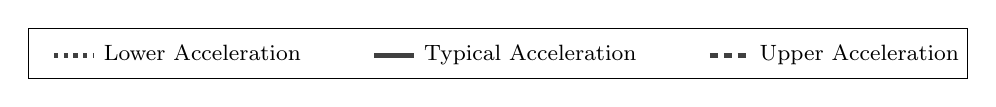
\begin{tikzpicture}
    \node[
        draw=black, line width=0.25pt,
        inner sep=3pt, rounded corners=0pt, align=center
    ] {%
        \footnotesize
        \setlength{\tabcolsep}{0pt}
        \renewcommand{\arraystretch}{1.3}
        \begin{tabular*}{\dimexpr0.95\linewidth}{
            @{\extracolsep{\fill}}
            c @{\extracolsep{0pt}\hspace{3pt}} l
            @{\extracolsep{\fill}}
            c @{\extracolsep{0pt}\hspace{3pt}} l
            @{\extracolsep{\fill}}
            c @{\extracolsep{0pt}\hspace{3pt}} l
            @{\extracolsep{\fill}}
        }
            \legline{gray!50!black}{dotted} & Lower Acceleration &
            \legline{gray!50!black}{solid} & Typical Acceleration &
            \legline{gray!50!black}{densely dashed} & Upper Acceleration \\
        \end{tabular*}%
    };
    \end{tikzpicture}}

    \vspace{-5pt}
    \caption{JIT guard fraction $\eta$ sensitivity ($d_{\text{link}} = 3$~m, Ideal Mechanical). Lower, Typical, and Upper Acceleration values are bolded: $0.5$, $9.5$, and $20$ m/s$^2$ (translational); $0.5$, $300$, and $700$ deg/s$^2$ (rotational).}
    \label{fig:reb_tuning_jiteta}
\end{figure}

\noindent For JIT, the guard fraction $\eta$ sets the trigger condition $\|\dot{\boldsymbol{\delta}}\| \cdot T_{\text{react}} > \eta \cdot \theta_{\text{HPBW}}$, controlling how far inside the Edge of Coverage the control frame is fired. Sweeping $\eta$ from $0.1$ to $0.7$ (Fig.~\ref{fig:reb_tuning_jiteta}), mean capacity stays within $\pm 5\%$ of its maximum across $\eta \in [0.25, 0.50]$. As $\eta$ grows, mean capacity falls off gradually because a larger guard fraction delays each realignment and lets the UE drift further off-axis before correcting. Below $\eta = 0.20$, the trigger fires too frequently and signaling overhead climbs sharply.\\

%-------------------------------------------------------------------%
\begin{tcbremark}
{\fontfamily{cmss}\selectfont
\blue{Analyze robustness of the trigger under long-term IMU drift without zero-velocity updates, and explain the effect of the 10\,ms IMU sampling period on sub-millisecond control reaction.}
}
\end{tcbremark}

\noindent JIT's robustness to long-term IMU drift depends on the IMU characteristics and the user's movement profile. Short bursts of motion allow opportunistic zero-velocity update (ZUPT) corrections that bound the bias, but in sustained continuous mobility without ZUPT opportunities the accumulated drift would otherwise degrade an IMU-only predictor over time.\\

\noindent Two design choices keep JIT robust in this regime. First, the pre-failure trigger,
\begin{equation}
    \|\dot{\boldsymbol{\delta}}\| \cdot T_{\text{react}} > \eta \cdot \theta_{\text{HPBW}}, \tag{Eq.~7}
\end{equation}
uses the Link Deviation \emph{velocity} $\|\dot{\boldsymbol{\delta}}\|$, so only a single accelerometer integration is required, avoiding the much faster double-integration drift incurred by position-based predictors. Second, JIT is not IMU-only: the RF link provides closed-loop verification at every slot, and a localized Hierarchical Search runs as a fallback whenever the IMU-based prediction underestimates a beam-edge crossing, so the link is never lost silently even in the presence of significant drift.\\

\noindent These design choices, limitations, and future-work directions on drift robustness are now stated explicitly in \emph{Methods/JIT Beam Realignment}; the relevant passage is reproduced below for the Reviewer's convenience.

\begin{quote}
{\color{cyan!75!black}
Two design choices limit the residual time-accumulated IMU drift in JIT. First, the trigger condition uses the Link Deviation \emph{velocity} rather than an absolute position, requiring only a single accelerometer integration and avoiding the double-integration drift that would otherwise accumulate with session length. Second, JIT is not IMU-only: the RF link provides closed-loop verification at every slot, and a localized Hierarchical Search runs as a fallback whenever the IMU-based prediction underestimates a beam-edge crossing, so the link is never lost silently. For sustained continuous-mobility scenarios, complementary bias-tracking from the inertial-navigation literature such as learning-based dead-reckoning~\cite{Brossard2020AIIMU}, deep-learning drift compensation~\cite{Chen2024DLInertial}, or zero-velocity detection~\cite{Skog2010ZUPT} would augment JIT's calibration as future work.
}
\end{quote}

\begin{figure}[ht!]
    \centering
    \begin{subfigure}{0.495\linewidth}
        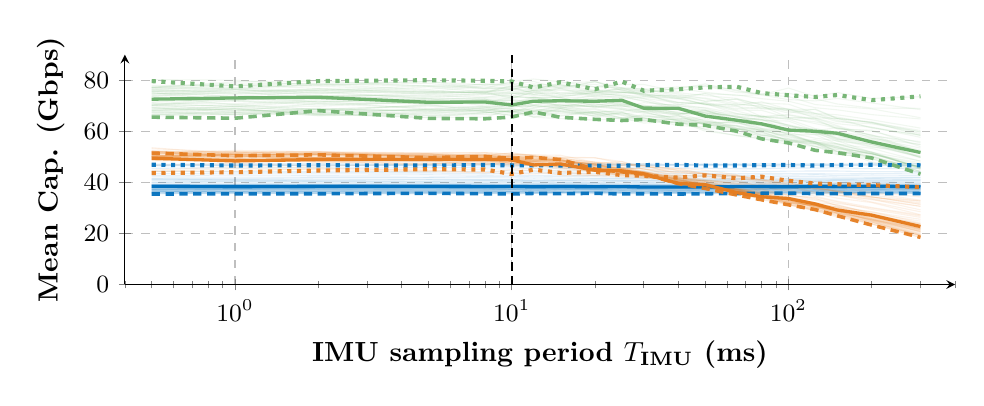
\begin{tikzpicture}
    \begin{axis}[width=\linewidth, height=4.5cm, xlabel={IMU sampling period $T_{\text{IMU}}$ (ms)}, ylabel={Mean Cap. (Gbps)}, xmin=0.4, xmax=400, ymin=0, ymax=90, every axis plot/.append style={mark=none}, xmode=log, log basis x=10,]
            \addplot[color=cb_blue, mark=none, opacity=0.10, line width=0.4pt, solid] coordinates {(0.5,46.62) (1,46.6) (2,46.74) (5,46.48) (8,46.87) (10,46.77) (12,46.5) (15,46.49) (20,46.78) (25,46.87) (30,46.68) (40,46.82) (50,46.88) (65,46.87) (80,46.55) (100,46.85) (125,46.54) (150,46.49) (200,46.81) (300,46.59)};
            \addplot[color=cb_blue, mark=none, opacity=0.10, line width=0.4pt, solid] coordinates {(0.5,46.98) (1,46.89) (2,47.06) (5,46.81) (8,46.9) (10,46.77) (12,46.79) (15,47.16) (20,46.91) (25,46.82) (30,46.98) (40,46.93) (50,46.88) (65,47.15) (80,46.85) (100,46.9) (125,47.02) (150,47.16) (200,47.12) (300,47.14)};
            \addplot[color=cb_blue, mark=none, opacity=0.10, line width=0.4pt, solid] coordinates {(0.5,47.1) (1,47.27) (2,47.32) (5,46.94) (8,47.38) (10,47.21) (12,47.33) (15,47.24) (20,47.37) (25,47.25) (30,47.3) (40,47.04) (50,47.19) (65,47.07) (80,47.38) (100,47.1) (125,47.31) (150,46.99) (200,47.34) (300,47.33)};
            \addplot[color=cb_blue, mark=none, opacity=0.10, line width=0.4pt, solid] coordinates {(0.5,46.47) (1,46.71) (2,46.47) (5,46.74) (8,46.41) (10,46.33) (12,46.67) (15,46.4) (20,46.39) (25,46.7) (30,46.71) (40,46.58) (50,46.7) (65,46.64) (80,46.48) (100,46.3) (125,46.69) (150,46.67) (200,46.73) (300,46.51)};
            \addplot[color=cb_blue, mark=none, opacity=0.10, line width=0.4pt, solid] coordinates {(0.5,45.5) (1,45.7) (2,45.64) (5,45.71) (8,45.69) (10,45.69) (12,45.63) (15,45.54) (20,45.47) (25,45.59) (30,45.68) (40,45.65) (50,45.52) (65,45.33) (80,45.34) (100,45.61) (125,45.6) (150,45.67) (200,45.38) (300,45.5)};
            \addplot[color=cb_blue, mark=none, opacity=0.10, line width=0.4pt, solid] coordinates {(0.5,44.36) (1,44.22) (2,44.12) (5,44.15) (8,44.31) (10,44.51) (12,44.45) (15,44.42) (20,44.45) (25,44.38) (30,44.43) (40,44.22) (50,44.29) (65,44.41) (80,44.2) (100,44.38) (125,44.45) (150,44.43) (200,44.17) (300,44.26)};
            \addplot[color=cb_blue, mark=none, opacity=0.10, line width=0.4pt, solid] coordinates {(0.5,43.34) (1,43.65) (2,43.68) (5,43.65) (8,43.36) (10,43.68) (12,43.67) (15,43.55) (20,43.54) (25,43.66) (30,43.69) (40,43.35) (50,43.57) (65,43.34) (80,43.44) (100,43.45) (125,43.38) (150,43.3) (200,43.42) (300,43.68)};
            \addplot[color=cb_blue, mark=none, opacity=0.10, line width=0.4pt, solid] coordinates {(0.5,42.62) (1,42.88) (2,42.76) (5,42.97) (8,42.77) (10,42.86) (12,42.62) (15,42.88) (20,42.65) (25,42.94) (30,42.91) (40,42.7) (50,42.78) (65,42.63) (80,42.94) (100,42.83) (125,43.0) (150,42.69) (200,42.86) (300,42.75)};
            \addplot[color=cb_blue, mark=none, opacity=0.10, line width=0.4pt, solid] coordinates {(0.5,42.13) (1,42.02) (2,42.08) (5,42.07) (8,42.22) (10,42.34) (12,42.12) (15,42.25) (20,42.15) (25,41.97) (30,42.02) (40,42.1) (50,42.25) (65,42.25) (80,42.26) (100,42.26) (125,42.27) (150,42.07) (200,42.0) (300,41.99)};
            \addplot[color=cb_blue, mark=none, opacity=0.10, line width=0.4pt, solid] coordinates {(0.5,41.5) (1,41.46) (2,41.74) (5,41.78) (8,41.76) (10,41.77) (12,41.62) (15,41.68) (20,41.39) (25,41.47) (30,41.62) (40,41.49) (50,41.53) (65,41.52) (80,41.77) (100,41.6) (125,41.61) (150,41.47) (200,41.58) (300,41.75)};
            \addplot[color=cb_blue, mark=none, opacity=0.10, line width=0.4pt, solid] coordinates {(0.5,41.33) (1,41.02) (2,41.1) (5,41.18) (8,41.02) (10,41.01) (12,40.98) (15,41.02) (20,41.33) (25,41.31) (30,41.27) (40,41.35) (50,41.08) (65,41.33) (80,41.22) (100,41.28) (125,41.07) (150,41.1) (200,41.33) (300,41.1)};
            \addplot[color=cb_blue, mark=none, opacity=0.10, line width=0.4pt, solid] coordinates {(0.5,41.06) (1,40.97) (2,40.72) (5,41.0) (8,40.92) (10,40.98) (12,40.68) (15,40.72) (20,40.75) (25,40.67) (30,40.76) (40,40.94) (50,40.83) (65,41.06) (80,41.03) (100,40.67) (125,40.8) (150,40.94) (200,40.85) (300,40.86)};
            \addplot[color=cb_blue, mark=none, opacity=0.10, line width=0.4pt, solid] coordinates {(0.5,40.78) (1,40.79) (2,40.49) (5,40.48) (8,40.79) (10,40.51) (12,40.51) (15,40.65) (20,40.55) (25,40.8) (30,40.68) (40,40.68) (50,40.83) (65,40.65) (80,40.67) (100,40.61) (125,40.47) (150,40.75) (200,40.71) (300,40.8)};
            \addplot[color=cb_blue, mark=none, opacity=0.10, line width=0.4pt, solid] coordinates {(0.5,40.09) (1,40.36) (2,40.36) (5,40.24) (8,40.32) (10,40.47) (12,40.42) (15,40.15) (20,40.12) (25,40.42) (30,40.35) (40,40.27) (50,40.47) (65,40.32) (80,40.09) (100,40.47) (125,40.35) (150,40.47) (200,40.21) (300,40.38)};
            \addplot[color=cb_blue, mark=none, opacity=0.10, line width=0.4pt, solid] coordinates {(0.5,40.09) (1,40.18) (2,40.02) (5,39.88) (8,39.82) (10,40.05) (12,39.92) (15,39.82) (20,39.82) (25,40.18) (30,39.95) (40,39.96) (50,39.87) (65,40.18) (80,40.14) (100,39.83) (125,40.14) (150,39.86) (200,40.11) (300,39.91)};
            \addplot[color=cb_blue, mark=none, opacity=0.10, line width=0.4pt, solid] coordinates {(0.5,39.73) (1,39.69) (2,39.48) (5,39.62) (8,39.6) (10,39.75) (12,39.55) (15,39.7) (20,39.48) (25,39.69) (30,39.76) (40,39.63) (50,39.62) (65,39.78) (80,39.62) (100,39.65) (125,39.6) (150,39.73) (200,39.75) (300,39.67)};
            \addplot[color=cb_blue, mark=none, opacity=0.10, line width=0.4pt, solid] coordinates {(0.5,39.33) (1,39.33) (2,39.18) (5,39.29) (8,39.34) (10,39.25) (12,39.43) (15,39.22) (20,39.35) (25,39.41) (30,39.37) (40,39.27) (50,39.33) (65,39.52) (80,39.35) (100,39.22) (125,39.21) (150,39.51) (200,39.49) (300,39.36)};
            \addplot[color=cb_blue, mark=none, opacity=0.10, line width=0.4pt, solid] coordinates {(0.5,39.09) (1,38.99) (2,39.0) (5,38.99) (8,39.01) (10,39.14) (12,39.01) (15,39.23) (20,39.19) (25,39.07) (30,39.07) (40,39.0) (50,39.17) (65,39.02) (80,39.23) (100,39.04) (125,39.04) (150,39.13) (200,39.0) (300,39.32)};
            \addplot[color=cb_blue, mark=none, opacity=0.10, line width=0.4pt, solid] coordinates {(0.5,38.96) (1,39.08) (2,39.02) (5,39.11) (8,39.09) (10,38.95) (12,39.22) (15,39.19) (20,38.92) (25,38.92) (30,39.14) (40,39.08) (50,39.19) (65,38.89) (80,39.06) (100,38.85) (125,38.89) (150,38.91) (200,39.03) (300,39.12)};
            \addplot[color=cb_blue, mark=none, opacity=0.10, line width=0.4pt, solid] coordinates {(0.5,39.07) (1,39.11) (2,38.97) (5,38.92) (8,38.97) (10,39.11) (12,38.87) (15,38.99) (20,39.0) (25,38.89) (30,38.85) (40,38.78) (50,38.74) (65,38.78) (80,38.74) (100,39.11) (125,39.07) (150,38.81) (200,38.98) (300,38.99)};
            \addplot[color=cb_blue, mark=none, opacity=0.10, line width=0.4pt, solid] coordinates {(0.5,38.78) (1,38.86) (2,38.92) (5,38.69) (8,38.73) (10,38.79) (12,38.8) (15,38.62) (20,38.68) (25,38.67) (30,38.89) (40,38.99) (50,38.8) (65,38.95) (80,38.84) (100,38.69) (125,38.83) (150,38.94) (200,38.63) (300,38.62)};
            \addplot[color=cb_blue, mark=none, opacity=0.10, line width=0.4pt, solid] coordinates {(0.5,38.68) (1,38.71) (2,38.81) (5,38.76) (8,38.72) (10,38.66) (12,38.65) (15,38.54) (20,38.62) (25,38.62) (30,38.66) (40,38.67) (50,38.69) (65,38.75) (80,38.62) (100,38.71) (125,38.64) (150,38.6) (200,38.55) (300,38.46)};
            \addplot[color=cb_blue, mark=none, opacity=0.10, line width=0.4pt, solid] coordinates {(0.5,38.56) (1,38.38) (2,38.4) (5,38.41) (8,38.58) (10,38.35) (12,38.48) (15,38.22) (20,38.33) (25,38.29) (30,38.35) (40,38.31) (50,38.3) (65,38.57) (80,38.35) (100,38.45) (125,38.54) (150,38.47) (200,38.27) (300,38.33)};
            \addplot[color=cb_blue, mark=none, opacity=0.10, line width=0.4pt, solid] coordinates {(0.5,38.39) (1,38.48) (2,38.44) (5,38.37) (8,38.4) (10,38.42) (12,38.42) (15,38.44) (20,38.36) (25,38.23) (30,38.4) (40,38.37) (50,38.17) (65,38.19) (80,38.35) (100,38.16) (125,38.28) (150,38.5) (200,38.23) (300,38.2)};
            \addplot[color=cb_blue, mark=none, opacity=0.10, line width=0.4pt, solid] coordinates {(0.5,37.94) (1,37.92) (2,38.25) (5,38.05) (8,37.98) (10,38.23) (12,38.26) (15,37.93) (20,37.94) (25,38.08) (30,38.15) (40,37.96) (50,38.0) (65,38.02) (80,38.05) (100,38.05) (125,37.93) (150,38.25) (200,38.02) (300,37.97)};
            \addplot[color=cb_blue, mark=none, opacity=0.10, line width=0.4pt, solid] coordinates {(0.5,38.02) (1,37.95) (2,38.01) (5,38.03) (8,38.11) (10,37.92) (12,37.93) (15,38.08) (20,37.8) (25,37.8) (30,37.99) (40,38.06) (50,38.12) (65,38.07) (80,37.77) (100,37.8) (125,38.0) (150,38.09) (200,38.1) (300,37.82)};
            \addplot[color=cb_blue, mark=none, opacity=0.10, line width=0.4pt, solid] coordinates {(0.5,37.72) (1,37.77) (2,37.8) (5,37.88) (8,37.64) (10,37.85) (12,37.73) (15,37.66) (20,37.93) (25,37.77) (30,37.76) (40,37.9) (50,37.7) (65,37.91) (80,37.73) (100,37.8) (125,37.64) (150,37.75) (200,37.89) (300,37.74)};
            \addplot[color=cb_blue, mark=none, opacity=0.10, line width=0.4pt, solid] coordinates {(0.5,37.78) (1,37.59) (2,37.81) (5,37.69) (8,37.62) (10,37.83) (12,37.69) (15,37.68) (20,37.7) (25,37.85) (30,37.83) (40,37.67) (50,37.54) (65,37.59) (80,37.53) (100,37.83) (125,37.89) (150,37.56) (200,37.65) (300,37.9)};
            \addplot[color=cb_blue, mark=none, opacity=0.10, line width=0.4pt, solid] coordinates {(0.5,37.55) (1,37.51) (2,37.77) (5,37.73) (8,37.73) (10,37.83) (12,37.51) (15,37.72) (20,37.75) (25,37.73) (30,37.68) (40,37.6) (50,37.64) (65,37.74) (80,37.69) (100,37.6) (125,37.76) (150,37.83) (200,37.49) (300,37.59)};
            \addplot[color=cb_blue, mark=none, opacity=0.10, line width=0.4pt, solid] coordinates {(0.5,37.57) (1,37.72) (2,37.64) (5,37.54) (8,37.45) (10,37.58) (12,37.67) (15,37.62) (20,37.64) (25,37.71) (30,37.67) (40,37.53) (50,37.45) (65,37.49) (80,37.39) (100,37.5) (125,37.65) (150,37.65) (200,37.42) (300,37.75)};
            \addplot[color=cb_blue, mark=none, opacity=0.10, line width=0.4pt, solid] coordinates {(0.5,37.43) (1,37.36) (2,37.53) (5,37.52) (8,37.61) (10,37.38) (12,37.33) (15,37.62) (20,37.54) (25,37.41) (30,37.61) (40,37.59) (50,37.69) (65,37.36) (80,37.34) (100,37.46) (125,37.56) (150,37.46) (200,37.34) (300,37.57)};
            \addplot[color=cb_blue, mark=none, opacity=0.10, line width=0.4pt, solid] coordinates {(0.5,37.31) (1,37.37) (2,37.54) (5,37.43) (8,37.63) (10,37.56) (12,37.63) (15,37.47) (20,37.6) (25,37.5) (30,37.46) (40,37.48) (50,37.39) (65,37.37) (80,37.55) (100,37.53) (125,37.51) (150,37.53) (200,37.46) (300,37.35)};
            \addplot[color=cb_blue, mark=none, opacity=0.10, line width=0.4pt, solid] coordinates {(0.5,37.31) (1,37.41) (2,37.5) (5,37.33) (8,37.23) (10,37.46) (12,37.5) (15,37.22) (20,37.21) (25,37.52) (30,37.37) (40,37.36) (50,37.33) (65,37.39) (80,37.41) (100,37.39) (125,37.34) (150,37.29) (200,37.38) (300,37.35)};
            \addplot[color=cb_blue, mark=none, opacity=0.10, line width=0.4pt, solid] coordinates {(0.5,37.24) (1,37.42) (2,37.26) (5,37.44) (8,37.38) (10,37.13) (12,37.12) (15,37.34) (20,37.12) (25,37.34) (30,37.4) (40,37.12) (50,37.15) (65,37.25) (80,37.35) (100,37.43) (125,37.21) (150,37.43) (200,37.3) (300,37.23)};
            \addplot[color=cb_blue, mark=none, opacity=0.10, line width=0.4pt, solid] coordinates {(0.5,36.99) (1,37.16) (2,36.96) (5,37.0) (8,37.08) (10,37.31) (12,37.06) (15,37.13) (20,37.24) (25,37.0) (30,37.17) (40,36.96) (50,37.28) (65,37.28) (80,37.03) (100,37.25) (125,37.13) (150,36.99) (200,37.08) (300,37.27)};
            \addplot[color=cb_blue, mark=none, opacity=0.10, line width=0.4pt, solid] coordinates {(0.5,37.1) (1,37.16) (2,37.16) (5,37.28) (8,37.24) (10,37.12) (12,37.21) (15,37.17) (20,37.23) (25,37.13) (30,37.12) (40,37.11) (50,37.11) (65,37.27) (80,37.07) (100,37.24) (125,37.19) (150,37.1) (200,37.03) (300,37.09)};
            \addplot[color=cb_blue, mark=none, opacity=0.10, line width=0.4pt, solid] coordinates {(0.5,37.0) (1,37.15) (2,37.13) (5,37.07) (8,37.04) (10,37.12) (12,37.06) (15,37.01) (20,37.09) (25,37.06) (30,37.01) (40,36.84) (50,37.01) (65,36.87) (80,37.03) (100,37.01) (125,36.82) (150,37.01) (200,36.87) (300,36.97)};
            \addplot[color=cb_blue, mark=none, opacity=0.10, line width=0.4pt, solid] coordinates {(0.5,37.07) (1,36.78) (2,37.08) (5,36.8) (8,36.74) (10,37.02) (12,36.82) (15,36.99) (20,37.06) (25,36.9) (30,37.03) (40,36.96) (50,36.88) (65,36.75) (80,37.05) (100,36.74) (125,36.9) (150,36.89) (200,37.05) (300,36.85)};
            \addplot[color=cb_blue, mark=none, opacity=0.10, line width=0.4pt, solid] coordinates {(0.5,36.74) (1,36.69) (2,36.69) (5,36.71) (8,36.7) (10,36.74) (12,36.68) (15,36.76) (20,36.8) (25,36.71) (30,36.88) (40,36.77) (50,36.66) (65,36.67) (80,36.79) (100,36.77) (125,36.8) (150,36.77) (200,36.79) (300,36.96)};
            \addplot[color=cb_blue, mark=none, opacity=0.10, line width=0.4pt, solid] coordinates {(0.5,36.58) (1,36.61) (2,36.81) (5,36.75) (8,36.71) (10,36.81) (12,36.67) (15,36.57) (20,36.55) (25,36.7) (30,36.68) (40,36.71) (50,36.68) (65,36.62) (80,36.86) (100,36.63) (125,36.89) (150,36.78) (200,36.62) (300,36.74)};
            \addplot[color=cb_blue, mark=none, opacity=0.10, line width=0.4pt, solid] coordinates {(0.5,36.66) (1,36.48) (2,36.52) (5,36.4) (8,36.61) (10,36.45) (12,36.73) (15,36.51) (20,36.73) (25,36.66) (30,36.57) (40,36.53) (50,36.71) (65,36.54) (80,36.37) (100,36.54) (125,36.68) (150,36.48) (200,36.73) (300,36.37)};
            \addplot[color=cb_blue, mark=none, opacity=0.10, line width=0.4pt, solid] coordinates {(0.5,36.52) (1,36.35) (2,36.4) (5,36.48) (8,36.32) (10,36.31) (12,36.41) (15,36.39) (20,36.36) (25,36.19) (30,36.45) (40,36.38) (50,36.29) (65,36.32) (80,36.22) (100,36.23) (125,36.38) (150,36.28) (200,36.34) (300,36.4)};
            \addplot[color=cb_blue, mark=none, opacity=0.10, line width=0.4pt, solid] coordinates {(0.5,36.45) (1,36.21) (2,36.35) (5,36.22) (8,36.19) (10,36.37) (12,36.26) (15,36.19) (20,36.46) (25,36.22) (30,36.27) (40,36.32) (50,36.1) (65,36.35) (80,36.33) (100,36.1) (125,36.27) (150,36.43) (200,36.34) (300,36.25)};
            \addplot[color=cb_blue, mark=none, opacity=0.10, line width=0.4pt, solid] coordinates {(0.5,36.43) (1,36.36) (2,36.38) (5,36.3) (8,36.39) (10,36.34) (12,36.13) (15,36.12) (20,36.41) (25,36.35) (30,36.35) (40,36.23) (50,36.4) (65,36.41) (80,36.24) (100,36.17) (125,36.38) (150,36.36) (200,36.11) (300,36.27)};
            \addplot[color=cb_blue, mark=none, opacity=0.10, line width=0.4pt, solid] coordinates {(0.5,36.36) (1,36.18) (2,36.1) (5,36.03) (8,36.12) (10,36.35) (12,36.15) (15,36.05) (20,36.24) (25,36.13) (30,36.28) (40,36.1) (50,36.2) (65,36.15) (80,36.12) (100,36.35) (125,36.27) (150,36.09) (200,36.09) (300,36.32)};
            \addplot[color=cb_blue, mark=none, opacity=0.10, line width=0.4pt, solid] coordinates {(0.5,36.04) (1,36.21) (2,36.1) (5,36.07) (8,36.1) (10,36.13) (12,36.1) (15,36.14) (20,36.1) (25,35.92) (30,35.94) (40,35.92) (50,35.99) (65,36.1) (80,35.98) (100,36.08) (125,36.18) (150,35.97) (200,36.14) (300,36.25)};
            \addplot[color=cb_blue, mark=none, opacity=0.10, line width=0.4pt, solid] coordinates {(0.5,36.05) (1,35.99) (2,35.89) (5,36.0) (8,35.96) (10,36.14) (12,36.03) (15,36.14) (20,35.82) (25,36.14) (30,35.95) (40,36.16) (50,35.9) (65,36.04) (80,35.97) (100,35.93) (125,36.07) (150,36.12) (200,35.88) (300,35.9)};
            \addplot[color=cb_blue, mark=none, opacity=0.10, line width=0.4pt, solid] coordinates {(0.5,35.84) (1,35.85) (2,35.69) (5,35.76) (8,35.72) (10,35.9) (12,35.7) (15,35.96) (20,36.04) (25,35.84) (30,35.72) (40,35.78) (50,35.75) (65,35.8) (80,35.92) (100,35.73) (125,35.86) (150,35.98) (200,35.9) (300,35.92)};
            \addplot[color=cb_blue, mark=none, opacity=0.10, line width=0.4pt, solid] coordinates {(0.5,35.67) (1,35.64) (2,35.59) (5,35.64) (8,35.68) (10,35.57) (12,35.67) (15,35.84) (20,35.89) (25,35.83) (30,35.77) (40,35.83) (50,35.78) (65,35.76) (80,35.58) (100,35.58) (125,35.57) (150,35.67) (200,35.86) (300,35.58)};
            \addplot[color=cb_blue, mark=none, opacity=0.10, line width=0.4pt, solid] coordinates {(0.5,35.47) (1,35.75) (2,35.58) (5,35.53) (8,35.65) (10,35.45) (12,35.67) (15,35.62) (20,35.53) (25,35.56) (30,35.46) (40,35.69) (50,35.51) (65,35.64) (80,35.66) (100,35.43) (125,35.56) (150,35.71) (200,35.74) (300,35.64)};
            \addplot[color=cb_orange, mark=none, opacity=0.10, line width=0.4pt, solid] coordinates {(0.5,44.19) (1,45.44) (2,45.02) (5,44.18) (8,43.85) (10,43.52) (12,43.21) (15,44.09) (20,42.59) (25,43.85) (30,42.29) (40,42.63) (50,42.38) (65,41.1) (80,41.04) (100,41.21) (125,40.18) (150,39.38) (200,39.84) (300,37.47)};
            \addplot[color=cb_orange, mark=none, opacity=0.10, line width=0.4pt, solid] coordinates {(0.5,44.22) (1,44.37) (2,45.41) (5,44.78) (8,43.72) (10,44.95) (12,44.52) (15,42.81) (20,42.62) (25,42.21) (30,41.84) (40,40.36) (50,40.94) (65,40.35) (80,38.49) (100,38.67) (125,38.56) (150,37.97) (200,36.15) (300,34.28)};
            \addplot[color=cb_orange, mark=none, opacity=0.10, line width=0.4pt, solid] coordinates {(0.5,44.74) (1,46.19) (2,45.75) (5,44.54) (8,45.17) (10,45.18) (12,45.59) (15,44.32) (20,43.05) (25,42.97) (30,43.24) (40,41.58) (50,40.41) (65,38.95) (80,38.74) (100,38.5) (125,36.18) (150,35.75) (200,34.13) (300,32.68)};
            \addplot[color=cb_orange, mark=none, opacity=0.10, line width=0.4pt, solid] coordinates {(0.5,46.66) (1,47.4) (2,46.31) (5,47.23) (8,47.61) (10,46.1) (12,46.79) (15,45.06) (20,44.22) (25,45.29) (30,43.27) (40,41.58) (50,40.6) (65,39.67) (80,39.1) (100,37.88) (125,37.54) (150,36.96) (200,34.19) (300,32.02)};
            \addplot[color=cb_orange, mark=none, opacity=0.10, line width=0.4pt, solid] coordinates {(0.5,48.49) (1,48.23) (2,49.76) (5,49.07) (8,48.01) (10,48.46) (12,47.26) (15,46.32) (20,47.34) (25,46.66) (30,43.92) (40,44.15) (50,42.47) (65,42.04) (80,39.6) (100,40.05) (125,37.59) (150,36.44) (200,35.77) (300,33.0)};
            \addplot[color=cb_orange, mark=none, opacity=0.10, line width=0.4pt, solid] coordinates {(0.5,51.3) (1,51.16) (2,50.97) (5,50.37) (8,50.21) (10,48.13) (12,48.01) (15,49.28) (20,47.95) (25,45.65) (30,45.29) (40,43.94) (50,43.31) (65,42.69) (80,40.02) (100,38.35) (125,38.11) (150,36.19) (200,34.97) (300,32.66)};
            \addplot[color=cb_orange, mark=none, opacity=0.10, line width=0.4pt, solid] coordinates {(0.5,50.6) (1,49.66) (2,51.29) (5,51.16) (8,50.93) (10,51.14) (12,50.58) (15,48.25) (20,46.88) (25,46.86) (30,46.45) (40,43.65) (50,43.44) (65,42.44) (80,40.97) (100,39.3) (125,37.83) (150,36.55) (200,34.33) (300,31.52)};
            \addplot[color=cb_orange, mark=none, opacity=0.10, line width=0.4pt, solid] coordinates {(0.5,52.2) (1,51.99) (2,51.16) (5,50.23) (8,50.39) (10,51.62) (12,50.4) (15,48.34) (20,47.67) (25,46.63) (30,47.28) (40,44.66) (50,43.2) (65,42.85) (80,40.86) (100,40.09) (125,37.47) (150,36.51) (200,33.69) (300,30.58)};
            \addplot[color=cb_orange, mark=none, opacity=0.10, line width=0.4pt, solid] coordinates {(0.5,52.28) (1,51.76) (2,52.09) (5,51.42) (8,51.63) (10,51.04) (12,50.76) (15,49.87) (20,49.65) (25,47.4) (30,46.61) (40,44.54) (50,43.34) (65,42.55) (80,40.57) (100,38.48) (125,38.34) (150,36.36) (200,34.37) (300,31.31)};
            \addplot[color=cb_orange, mark=none, opacity=0.10, line width=0.4pt, solid] coordinates {(0.5,53.57) (1,51.11) (2,50.76) (5,50.31) (8,50.54) (10,50.44) (12,50.38) (15,49.55) (20,49.58) (25,48.14) (30,46.19) (40,45.51) (50,44.74) (65,42.97) (80,41.0) (100,39.35) (125,37.98) (150,34.93) (200,33.19) (300,30.64)};
            \addplot[color=cb_orange, mark=none, opacity=0.10, line width=0.4pt, solid] coordinates {(0.5,53.16) (1,51.87) (2,51.59) (5,51.65) (8,51.64) (10,51.08) (12,50.77) (15,50.6) (20,47.82) (25,47.29) (30,45.89) (40,45.37) (50,43.32) (65,41.63) (80,40.69) (100,38.96) (125,37.16) (150,35.24) (200,33.44) (300,29.22)};
            \addplot[color=cb_orange, mark=none, opacity=0.10, line width=0.4pt, solid] coordinates {(0.5,51.29) (1,52.5) (2,52.01) (5,50.36) (8,50.78) (10,50.96) (12,50.07) (15,49.77) (20,47.39) (25,48.17) (30,44.96) (40,45.03) (50,43.6) (65,40.73) (80,39.4) (100,38.22) (125,35.95) (150,35.14) (200,32.31) (300,28.47)};
            \addplot[color=cb_orange, mark=none, opacity=0.10, line width=0.4pt, solid] coordinates {(0.5,50.33) (1,51.99) (2,52.03) (5,49.68) (8,51.49) (10,49.82) (12,50.15) (15,49.26) (20,47.95) (25,47.38) (30,46.57) (40,43.06) (50,41.99) (65,40.45) (80,38.25) (100,36.42) (125,35.51) (150,33.81) (200,32.08) (300,27.32)};
            \addplot[color=cb_orange, mark=none, opacity=0.10, line width=0.4pt, solid] coordinates {(0.5,50.06) (1,50.9) (2,49.28) (5,50.52) (8,49.82) (10,48.97) (12,48.25) (15,49.61) (20,46.65) (25,45.36) (30,45.28) (40,42.19) (50,40.7) (65,39.8) (80,37.6) (100,37.15) (125,34.55) (150,32.63) (200,30.14) (300,27.18)};
            \addplot[color=cb_orange, mark=none, opacity=0.10, line width=0.4pt, solid] coordinates {(0.5,50.48) (1,49.14) (2,51.05) (5,50.41) (8,48.38) (10,48.47) (12,48.59) (15,48.43) (20,46.53) (25,45.63) (30,45.3) (40,42.7) (50,41.01) (65,39.49) (80,37.15) (100,34.95) (125,33.42) (150,31.8) (200,29.88) (300,26.79)};
            \addplot[color=cb_orange, mark=none, opacity=0.10, line width=0.4pt, solid] coordinates {(0.5,50.22) (1,50.86) (2,50.46) (5,49.01) (8,49.09) (10,49.38) (12,47.85) (15,48.43) (20,46.07) (25,45.41) (30,44.35) (40,41.63) (50,40.76) (65,39.24) (80,36.46) (100,34.86) (125,34.15) (150,32.32) (200,29.38) (300,26.29)};
            \addplot[color=cb_orange, mark=none, opacity=0.10, line width=0.4pt, solid] coordinates {(0.5,49.03) (1,49.67) (2,48.93) (5,49.86) (8,47.93) (10,49.35) (12,47.47) (15,47.47) (20,45.32) (25,45.51) (30,43.92) (40,42.11) (50,39.54) (65,38.18) (80,37.51) (100,34.93) (125,33.81) (150,30.78) (200,28.35) (300,25.53)};
            \addplot[color=cb_orange, mark=none, opacity=0.10, line width=0.4pt, solid] coordinates {(0.5,49.22) (1,49.22) (2,48.41) (5,48.61) (8,48.29) (10,47.25) (12,48.29) (15,47.56) (20,45.32) (25,44.9) (30,44.03) (40,41.17) (50,38.86) (65,37.17) (80,37.05) (100,34.2) (125,33.04) (150,31.04) (200,27.89) (300,24.8)};
            \addplot[color=cb_orange, mark=none, opacity=0.10, line width=0.4pt, solid] coordinates {(0.5,49.12) (1,50.55) (2,48.23) (5,49.47) (8,49.29) (10,47.56) (12,46.75) (15,46.09) (20,45.16) (25,44.45) (30,43.02) (40,40.48) (50,40.3) (65,38.15) (80,35.55) (100,34.11) (125,32.0) (150,30.15) (200,28.52) (300,24.1)};
            \addplot[color=cb_orange, mark=none, opacity=0.10, line width=0.4pt, solid] coordinates {(0.5,50.13) (1,50.14) (2,49.75) (5,48.89) (8,48.85) (10,49.18) (12,47.5) (15,46.43) (20,44.44) (25,43.1) (30,43.65) (40,41.7) (50,40.4) (65,37.33) (80,35.44) (100,33.37) (125,32.03) (150,31.29) (200,27.69) (300,23.68)};
            \addplot[color=cb_orange, mark=none, opacity=0.10, line width=0.4pt, solid] coordinates {(0.5,49.94) (1,48.5) (2,49.79) (5,49.14) (8,48.99) (10,47.29) (12,46.83) (15,46.54) (20,44.41) (25,43.64) (30,43.02) (40,40.31) (50,38.75) (65,37.4) (80,36.44) (100,33.15) (125,31.41) (150,30.02) (200,27.13) (300,23.56)};
            \addplot[color=cb_orange, mark=none, opacity=0.10, line width=0.4pt, solid] coordinates {(0.5,48.88) (1,48.73) (2,48.57) (5,47.18) (8,48.76) (10,48.25) (12,47.11) (15,45.52) (20,44.45) (25,43.36) (30,42.86) (40,41.67) (50,38.29) (65,37.11) (80,36.23) (100,34.07) (125,31.02) (150,30.59) (200,27.36) (300,23.85)};
            \addplot[color=cb_orange, mark=none, opacity=0.10, line width=0.4pt, solid] coordinates {(0.5,49.73) (1,49.35) (2,49.72) (5,48.6) (8,47.5) (10,48.12) (12,48.23) (15,45.99) (20,45.75) (25,43.62) (30,42.15) (40,40.74) (50,39.05) (65,36.62) (80,35.39) (100,32.81) (125,31.42) (150,30.36) (200,26.58) (300,23.1)};
            \addplot[color=cb_orange, mark=none, opacity=0.10, line width=0.4pt, solid] coordinates {(0.5,50.25) (1,48.46) (2,49.17) (5,48.76) (8,48.2) (10,46.75) (12,47.02) (15,45.94) (20,44.15) (25,42.97) (30,41.46) (40,41.31) (50,38.98) (65,37.55) (80,35.43) (100,32.82) (125,30.77) (150,29.65) (200,27.06) (300,22.73)};
            \addplot[color=cb_orange, mark=none, opacity=0.10, line width=0.4pt, solid] coordinates {(0.5,50.5) (1,49.34) (2,48.12) (5,47.03) (8,48.78) (10,47.43) (12,46.74) (15,46.52) (20,45.85) (25,43.96) (30,41.89) (40,40.78) (50,39.15) (65,36.84) (80,34.7) (100,32.68) (125,30.88) (150,28.55) (200,27.01) (300,21.98)};
            \addplot[color=cb_orange, mark=none, opacity=0.10, line width=0.4pt, solid] coordinates {(0.5,48.59) (1,49.33) (2,47.78) (5,47.48) (8,46.98) (10,48.07) (12,48.14) (15,47.43) (20,44.33) (25,42.66) (30,42.86) (40,39.97) (50,39.08) (65,36.08) (80,34.23) (100,32.43) (125,30.48) (150,29.03) (200,26.5) (300,21.97)};
            \addplot[color=cb_orange, mark=none, opacity=0.10, line width=0.4pt, solid] coordinates {(0.5,50.07) (1,47.99) (2,49.82) (5,47.96) (8,47.17) (10,47.72) (12,47.38) (15,46.97) (20,45.49) (25,44.24) (30,42.96) (40,39.32) (50,38.34) (65,37.09) (80,35.13) (100,33.4) (125,30.81) (150,28.44) (200,26.42) (300,21.72)};
            \addplot[color=cb_orange, mark=none, opacity=0.10, line width=0.4pt, solid] coordinates {(0.5,49.39) (1,49.01) (2,48.47) (5,48.56) (8,47.04) (10,47.08) (12,47.38) (15,45.7) (20,44.27) (25,42.53) (30,42.37) (40,40.75) (50,38.55) (65,37.19) (80,35.39) (100,33.4) (125,30.37) (150,28.81) (200,26.17) (300,21.9)};
            \addplot[color=cb_orange, mark=none, opacity=0.10, line width=0.4pt, solid] coordinates {(0.5,49.58) (1,48.31) (2,50.13) (5,48.34) (8,48.53) (10,47.52) (12,47.6) (15,46.21) (20,46.16) (25,44.32) (30,42.61) (40,40.46) (50,39.1) (65,36.91) (80,35.0) (100,33.41) (125,30.98) (150,28.48) (200,25.36) (300,22.06)};
            \addplot[color=cb_orange, mark=none, opacity=0.10, line width=0.4pt, solid] coordinates {(0.5,50.34) (1,50.08) (2,49.77) (5,49.15) (8,47.97) (10,48.33) (12,48.36) (15,46.37) (20,45.6) (25,44.95) (30,43.44) (40,39.58) (50,39.32) (65,36.85) (80,35.48) (100,32.54) (125,30.72) (150,29.37) (200,25.9) (300,21.25)};
            \addplot[color=cb_orange, mark=none, opacity=0.10, line width=0.4pt, solid] coordinates {(0.5,50.08) (1,50.73) (2,48.92) (5,48.56) (8,49.94) (10,49.06) (12,47.88) (15,46.72) (20,45.37) (25,44.97) (30,43.36) (40,39.88) (50,39.18) (65,37.19) (80,34.55) (100,32.17) (125,30.98) (150,29.41) (200,25.7) (300,21.28)};
            \addplot[color=cb_orange, mark=none, opacity=0.10, line width=0.4pt, solid] coordinates {(0.5,51.54) (1,50.73) (2,48.34) (5,48.02) (8,49.31) (10,48.77) (12,48.56) (15,47.74) (20,44.83) (25,43.86) (30,43.3) (40,40.07) (50,38.25) (65,37.44) (80,34.66) (100,33.17) (125,30.01) (150,28.03) (200,25.27) (300,21.57)};
            \addplot[color=cb_orange, mark=none, opacity=0.10, line width=0.4pt, solid] coordinates {(0.5,50.01) (1,51.25) (2,49.63) (5,49.68) (8,49.41) (10,49.89) (12,47.65) (15,46.96) (20,45.53) (25,43.86) (30,42.72) (40,41.03) (50,38.98) (65,37.05) (80,34.15) (100,32.01) (125,30.91) (150,27.97) (200,25.77) (300,21.74)};
            \addplot[color=cb_orange, mark=none, opacity=0.10, line width=0.4pt, solid] coordinates {(0.5,49.99) (1,50.7) (2,49.02) (5,50.01) (8,50.7) (10,50.02) (12,49.89) (15,47.74) (20,45.78) (25,44.51) (30,43.08) (40,41.92) (50,40.24) (65,37.52) (80,35.79) (100,33.14) (125,30.45) (150,28.12) (200,25.51) (300,21.01)};
            \addplot[color=cb_orange, mark=none, opacity=0.10, line width=0.4pt, solid] coordinates {(0.5,50.37) (1,50.91) (2,51.13) (5,50.68) (8,50.82) (10,48.83) (12,49.43) (15,49.03) (20,45.95) (25,45.41) (30,44.32) (40,41.09) (50,39.71) (65,37.42) (80,35.13) (100,32.85) (125,30.25) (150,29.53) (200,26.31) (300,21.49)};
            \addplot[color=cb_orange, mark=none, opacity=0.10, line width=0.4pt, solid] coordinates {(0.5,50.36) (1,50.85) (2,49.67) (5,51.08) (8,49.6) (10,49.77) (12,49.62) (15,48.07) (20,46.88) (25,44.15) (30,43.6) (40,42.35) (50,40.4) (65,38.08) (80,35.84) (100,33.68) (125,31.08) (150,28.5) (200,25.27) (300,20.67)};
            \addplot[color=cb_orange, mark=none, opacity=0.10, line width=0.4pt, solid] coordinates {(0.5,51.66) (1,51.4) (2,51.72) (5,50.31) (8,49.1) (10,50.64) (12,48.86) (15,48.71) (20,46.7) (25,45.91) (30,42.98) (40,41.29) (50,38.72) (65,37.4) (80,34.66) (100,32.42) (125,30.99) (150,28.89) (200,24.99) (300,20.8)};
            \addplot[color=cb_orange, mark=none, opacity=0.10, line width=0.4pt, solid] coordinates {(0.5,52.1) (1,50.28) (2,51.84) (5,51.24) (8,50.62) (10,49.13) (12,48.68) (15,48.16) (20,47.42) (25,44.12) (30,42.81) (40,41.36) (50,39.8) (65,36.21) (80,35.31) (100,33.36) (125,31.1) (150,28.87) (200,25.45) (300,20.81)};
            \addplot[color=cb_orange, mark=none, opacity=0.10, line width=0.4pt, solid] coordinates {(0.5,51.16) (1,51.63) (2,51.28) (5,49.86) (8,50.24) (10,49.91) (12,50.08) (15,48.88) (20,45.77) (25,44.01) (30,42.61) (40,40.33) (50,39.71) (65,37.64) (80,35.26) (100,31.97) (125,30.08) (150,28.83) (200,25.72) (300,20.54)};
            \addplot[color=cb_orange, mark=none, opacity=0.10, line width=0.4pt, solid] coordinates {(0.5,50.17) (1,49.94) (2,50.75) (5,51.0) (8,51.05) (10,49.28) (12,48.84) (15,48.53) (20,47.05) (25,44.86) (30,43.67) (40,40.54) (50,38.96) (65,36.81) (80,34.66) (100,31.91) (125,30.82) (150,28.67) (200,24.99) (300,20.24)};
            \addplot[color=cb_orange, mark=none, opacity=0.10, line width=0.4pt, solid] coordinates {(0.5,51.72) (1,50.15) (2,51.08) (5,50.88) (8,50.36) (10,49.97) (12,48.69) (15,49.26) (20,45.47) (25,45.9) (30,43.86) (40,41.01) (50,39.74) (65,36.66) (80,35.0) (100,32.19) (125,30.77) (150,27.84) (200,25.26) (300,19.83)};
            \addplot[color=cb_orange, mark=none, opacity=0.10, line width=0.4pt, solid] coordinates {(0.5,52.02) (1,51.81) (2,51.12) (5,48.96) (8,50.72) (10,48.88) (12,49.08) (15,47.77) (20,47.4) (25,45.08) (30,44.09) (40,41.98) (50,39.1) (65,36.27) (80,34.84) (100,33.06) (125,30.3) (150,27.78) (200,24.73) (300,19.73)};
            \addplot[color=cb_orange, mark=none, opacity=0.10, line width=0.4pt, solid] coordinates {(0.5,51.89) (1,50.21) (2,51.48) (5,49.78) (8,48.85) (10,50.26) (12,49.26) (15,48.71) (20,47.03) (25,45.13) (30,43.17) (40,40.2) (50,38.21) (65,36.82) (80,34.06) (100,31.58) (125,29.36) (150,28.14) (200,24.84) (300,19.29)};
            \addplot[color=cb_orange, mark=none, opacity=0.10, line width=0.4pt, solid] coordinates {(0.5,51.93) (1,51.14) (2,50.99) (5,51.22) (8,48.85) (10,50.71) (12,48.84) (15,48.75) (20,47.15) (25,43.69) (30,44.22) (40,40.16) (50,37.96) (65,37.24) (80,34.58) (100,32.18) (125,30.36) (150,27.84) (200,24.29) (300,19.15)};
            \addplot[color=cb_orange, mark=none, opacity=0.10, line width=0.4pt, solid] coordinates {(0.5,50.72) (1,50.95) (2,51.04) (5,51.16) (8,50.13) (10,49.31) (12,49.51) (15,48.65) (20,46.54) (25,45.21) (30,43.97) (40,41.1) (50,38.36) (65,36.6) (80,34.03) (100,31.35) (125,28.96) (150,27.55) (200,24.5) (300,19.48)};
            \addplot[color=cb_orange, mark=none, opacity=0.10, line width=0.4pt, solid] coordinates {(0.5,50.14) (1,51.14) (2,50.73) (5,49.44) (8,50.34) (10,50.32) (12,48.23) (15,47.88) (20,46.47) (25,44.4) (30,43.29) (40,39.91) (50,37.88) (65,36.98) (80,34.67) (100,31.36) (125,29.93) (150,26.79) (200,24.23) (300,19.35)};
            \addplot[color=cb_orange, mark=none, opacity=0.10, line width=0.4pt, solid] coordinates {(0.5,52.19) (1,50.95) (2,50.61) (5,50.23) (8,50.27) (10,50.32) (12,48.1) (15,48.52) (20,47.2) (25,45.42) (30,42.42) (40,40.9) (50,38.06) (65,36.28) (80,34.62) (100,31.19) (125,28.83) (150,26.95) (200,23.64) (300,19.24)};
            \addplot[color=cb_orange, mark=none, opacity=0.10, line width=0.4pt, solid] coordinates {(0.5,52.3) (1,49.8) (2,51.78) (5,50.04) (8,49.4) (10,49.72) (12,48.84) (15,48.98) (20,44.96) (25,44.07) (30,44.05) (40,40.7) (50,39.18) (65,36.41) (80,33.94) (100,31.83) (125,29.57) (150,27.28) (200,24.51) (300,18.9)};
            \addplot[color=cb_orange, mark=none, opacity=0.10, line width=0.4pt, solid] coordinates {(0.5,51.45) (1,50.2) (2,49.51) (5,50.77) (8,49.04) (10,48.78) (12,48.48) (15,48.65) (20,47.11) (25,44.67) (30,42.4) (40,40.29) (50,37.83) (65,36.25) (80,33.21) (100,31.21) (125,29.0) (150,27.67) (200,23.68) (300,18.5)};
            \addplot[color=cb_orange, mark=none, opacity=0.10, line width=0.4pt, solid] coordinates {(0.5,50.69) (1,50.71) (2,50.98) (5,50.03) (8,48.59) (10,50.09) (12,50.14) (15,48.28) (20,45.3) (25,44.1) (30,43.29) (40,41.16) (50,38.67) (65,35.8) (80,33.25) (100,32.27) (125,28.96) (150,26.37) (200,23.79) (300,18.35)};
            \addplot[color=cb_green, mark=none, opacity=0.10, line width=0.4pt, solid] coordinates {(0.5,76.62) (1,76.56) (2,78.28) (5,76.39) (8,78.63) (10,77.55) (12,77.44) (15,77.2) (20,79.39) (25,76.68) (30,75.64) (40,76.66) (50,78.56) (65,75.8) (80,74.34) (100,76.94) (125,73.59) (150,75.19) (200,72.85) (300,73.54)};
            \addplot[color=cb_green, mark=none, opacity=0.10, line width=0.4pt, solid] coordinates {(0.5,77.93) (1,78.08) (2,78.75) (5,79.39) (8,78.17) (10,78.38) (12,79.51) (15,76.68) (20,79.49) (25,77.01) (30,76.5) (40,77.38) (50,77.64) (65,75.21) (80,74.76) (100,74.91) (125,72.69) (150,70.7) (200,69.08) (300,68.99)};
            \addplot[color=cb_green, mark=none, opacity=0.10, line width=0.4pt, solid] coordinates {(0.5,77.25) (1,77.14) (2,78.13) (5,79.53) (8,76.85) (10,79.49) (12,80.47) (15,79.42) (20,77.36) (25,78.37) (30,78.33) (40,75.52) (50,77.85) (65,76.16) (80,74.2) (100,72.4) (125,71.91) (150,72.84) (200,71.07) (300,68.47)};
            \addplot[color=cb_green, mark=none, opacity=0.10, line width=0.4pt, solid] coordinates {(0.5,77.24) (1,79.4) (2,79.75) (5,77.64) (8,77.27) (10,76.4) (12,76.36) (15,78.9) (20,79.43) (25,75.96) (30,75.09) (40,76.81) (50,75.27) (65,73.95) (80,74.39) (100,73.59) (125,70.47) (150,69.75) (200,68.78) (300,65.31)};
            \addplot[color=cb_green, mark=none, opacity=0.10, line width=0.4pt, solid] coordinates {(0.5,77.04) (1,78.9) (2,78.48) (5,77.74) (8,76.62) (10,77.43) (12,78.56) (15,77.93) (20,77.48) (25,76.95) (30,76.62) (40,73.74) (50,74.69) (65,74.27) (80,72.77) (100,71.76) (125,69.23) (150,68.4) (200,66.53) (300,64.82)};
            \addplot[color=cb_green, mark=none, opacity=0.10, line width=0.4pt, solid] coordinates {(0.5,77.36) (1,78.15) (2,76.78) (5,75.63) (8,75.06) (10,77.99) (12,76.74) (15,78.42) (20,76.05) (25,75.37) (30,74.81) (40,72.81) (50,74.82) (65,71.14) (80,71.09) (100,70.61) (125,67.01) (150,66.46) (200,64.48) (300,61.24)};
            \addplot[color=cb_green, mark=none, opacity=0.10, line width=0.4pt, solid] coordinates {(0.5,77.1) (1,76.46) (2,75.12) (5,75.45) (8,77.84) (10,76.74) (12,77.43) (15,74.42) (20,75.69) (25,75.74) (30,74.68) (40,73.1) (50,73.06) (65,70.71) (80,69.66) (100,67.13) (125,68.72) (150,65.12) (200,63.62) (300,59.7)};
            \addplot[color=cb_green, mark=none, opacity=0.10, line width=0.4pt, solid] coordinates {(0.5,76.57) (1,75.01) (2,76.66) (5,75.28) (8,75.16) (10,76.56) (12,75.28) (15,77.2) (20,75.18) (25,75.26) (30,74.3) (40,73.64) (50,71.7) (65,72.59) (80,68.89) (100,68.65) (125,68.49) (150,64.93) (200,63.39) (300,60.32)};
            \addplot[color=cb_green, mark=none, opacity=0.10, line width=0.4pt, solid] coordinates {(0.5,74.56) (1,76.48) (2,73.96) (5,73.92) (8,73.36) (10,74.69) (12,76.0) (15,76.59) (20,73.43) (25,73.01) (30,73.44) (40,72.94) (50,70.44) (65,69.59) (80,68.8) (100,68.2) (125,66.36) (150,63.77) (200,62.92) (300,59.82)};
            \addplot[color=cb_green, mark=none, opacity=0.10, line width=0.4pt, solid] coordinates {(0.5,76.39) (1,78.0) (2,77.69) (5,75.95) (8,74.89) (10,74.88) (12,74.55) (15,75.06) (20,75.97) (25,76.37) (30,73.74) (40,74.15) (50,71.8) (65,72.57) (80,70.41) (100,67.85) (125,65.76) (150,65.02) (200,63.53) (300,58.39)};
            \addplot[color=cb_green, mark=none, opacity=0.10, line width=0.4pt, solid] coordinates {(0.5,75.54) (1,76.92) (2,75.92) (5,77.91) (8,78.28) (10,78.78) (12,75.91) (15,78.11) (20,75.31) (25,76.61) (30,76.33) (40,74.63) (50,72.73) (65,70.05) (80,71.56) (100,68.59) (125,67.05) (150,64.27) (200,61.56) (300,57.64)};
            \addplot[color=cb_green, mark=none, opacity=0.10, line width=0.4pt, solid] coordinates {(0.5,80.24) (1,80.0) (2,78.03) (5,78.78) (8,76.72) (10,76.56) (12,77.96) (15,77.56) (20,78.4) (25,76.18) (30,75.9) (40,75.11) (50,74.01) (65,72.88) (80,70.26) (100,68.52) (125,66.83) (150,65.56) (200,63.25) (300,59.09)};
            \addplot[color=cb_green, mark=none, opacity=0.10, line width=0.4pt, solid] coordinates {(0.5,74.77) (1,74.74) (2,74.78) (5,77.43) (8,75.39) (10,76.39) (12,78.06) (15,74.97) (20,74.86) (25,77.08) (30,74.19) (40,72.65) (50,70.69) (65,68.82) (80,69.31) (100,68.72) (125,65.19) (150,65.0) (200,61.25) (300,58.61)};
            \addplot[color=cb_green, mark=none, opacity=0.10, line width=0.4pt, solid] coordinates {(0.5,76.03) (1,75.43) (2,76.49) (5,74.82) (8,75.48) (10,77.39) (12,74.52) (15,76.84) (20,74.04) (25,75.12) (30,75.62) (40,73.3) (50,70.4) (65,70.59) (80,69.91) (100,65.37) (125,65.17) (150,62.98) (200,61.58) (300,58.36)};
            \addplot[color=cb_green, mark=none, opacity=0.10, line width=0.4pt, solid] coordinates {(0.5,73.58) (1,75.52) (2,72.99) (5,73.54) (8,74.88) (10,73.77) (12,76.1) (15,76.02) (20,75.76) (25,75.32) (30,74.31) (40,71.32) (50,71.04) (65,70.04) (80,65.75) (100,65.27) (125,65.13) (150,62.22) (200,58.2) (300,55.95)};
            \addplot[color=cb_green, mark=none, opacity=0.10, line width=0.4pt, solid] coordinates {(0.5,75.65) (1,73.52) (2,73.21) (5,75.16) (8,76.02) (10,75.64) (12,75.82) (15,74.53) (20,75.14) (25,75.13) (30,74.77) (40,70.46) (50,71.28) (65,68.32) (80,68.2) (100,65.24) (125,63.02) (150,61.19) (200,58.51) (300,54.71)};
            \addplot[color=cb_green, mark=none, opacity=0.10, line width=0.4pt, solid] coordinates {(0.5,75.51) (1,76.2) (2,75.86) (5,74.61) (8,75.55) (10,74.87) (12,74.04) (15,73.73) (20,75.09) (25,73.81) (30,71.68) (40,69.85) (50,69.27) (65,66.91) (80,65.83) (100,66.54) (125,64.8) (150,61.13) (200,60.02) (300,55.46)};
            \addplot[color=cb_green, mark=none, opacity=0.10, line width=0.4pt, solid] coordinates {(0.5,74.0) (1,76.15) (2,75.07) (5,73.07) (8,74.37) (10,75.33) (12,74.45) (15,73.38) (20,75.23) (25,73.94) (30,73.82) (40,71.25) (50,70.67) (65,67.94) (80,65.55) (100,66.31) (125,64.43) (150,60.91) (200,60.42) (300,53.99)};
            \addplot[color=cb_green, mark=none, opacity=0.10, line width=0.4pt, solid] coordinates {(0.5,76.09) (1,74.48) (2,76.12) (5,75.38) (8,75.38) (10,72.88) (12,75.26) (15,73.9) (20,74.43) (25,74.5) (30,72.89) (40,71.14) (50,70.75) (65,66.96) (80,65.62) (100,64.89) (125,63.7) (150,61.86) (200,57.34) (300,53.43)};
            \addplot[color=cb_green, mark=none, opacity=0.10, line width=0.4pt, solid] coordinates {(0.5,75.01) (1,73.68) (2,75.66) (5,72.66) (8,72.99) (10,73.0) (12,75.51) (15,73.01) (20,73.65) (25,73.8) (30,72.74) (40,69.05) (50,68.25) (65,66.57) (80,65.77) (100,64.69) (125,61.08) (150,59.47) (200,57.25) (300,54.85)};
            \addplot[color=cb_green, mark=none, opacity=0.10, line width=0.4pt, solid] coordinates {(0.5,75.21) (1,72.01) (2,73.58) (5,74.31) (8,74.61) (10,73.86) (12,73.03) (15,71.72) (20,74.19) (25,73.22) (30,72.03) (40,68.45) (50,67.85) (65,65.55) (80,64.24) (100,64.02) (125,60.2) (150,61.44) (200,58.56) (300,51.95)};
            \addplot[color=cb_green, mark=none, opacity=0.10, line width=0.4pt, solid] coordinates {(0.5,74.25) (1,72.79) (2,74.15) (5,72.29) (8,73.32) (10,73.62) (12,73.18) (15,72.15) (20,72.29) (25,70.92) (30,69.81) (40,70.59) (50,69.01) (65,65.53) (80,66.29) (100,62.16) (125,60.86) (150,59.83) (200,57.94) (300,51.74)};
            \addplot[color=cb_green, mark=none, opacity=0.10, line width=0.4pt, solid] coordinates {(0.5,73.58) (1,70.38) (2,71.83) (5,70.82) (8,72.65) (10,71.1) (12,73.46) (15,71.68) (20,72.98) (25,72.02) (30,68.76) (40,67.51) (50,66.0) (65,64.23) (80,65.45) (100,61.75) (125,60.61) (150,57.48) (200,56.98) (300,52.61)};
            \addplot[color=cb_green, mark=none, opacity=0.10, line width=0.4pt, solid] coordinates {(0.5,72.88) (1,71.84) (2,70.32) (5,71.58) (8,71.83) (10,72.11) (12,70.22) (15,72.07) (20,70.28) (25,71.37) (30,68.96) (40,66.67) (50,68.06) (65,65.42) (80,64.72) (100,62.51) (125,60.25) (150,56.72) (200,53.77) (300,51.96)};
            \addplot[color=cb_green, mark=none, opacity=0.10, line width=0.4pt, solid] coordinates {(0.5,70.18) (1,71.99) (2,70.79) (5,71.04) (8,72.22) (10,72.45) (12,71.35) (15,69.89) (20,71.22) (25,71.82) (30,68.66) (40,66.55) (50,68.24) (65,63.77) (80,62.87) (100,60.86) (125,59.24) (150,58.33) (200,54.71) (300,51.37)};
            \addplot[color=cb_green, mark=none, opacity=0.10, line width=0.4pt, solid] coordinates {(0.5,71.45) (1,73.14) (2,72.61) (5,71.14) (8,71.76) (10,72.04) (12,72.18) (15,72.17) (20,72.7) (25,70.4) (30,70.3) (40,68.24) (50,67.39) (65,65.93) (80,64.49) (100,62.48) (125,59.07) (150,56.7) (200,56.63) (300,49.64)};
            \addplot[color=cb_green, mark=none, opacity=0.10, line width=0.4pt, solid] coordinates {(0.5,72.22) (1,73.65) (2,73.52) (5,70.42) (8,71.46) (10,73.26) (12,73.33) (15,73.16) (20,70.77) (25,69.49) (30,71.19) (40,70.04) (50,68.42) (65,64.35) (80,64.63) (100,60.35) (125,58.63) (150,59.32) (200,55.63) (300,50.33)};
            \addplot[color=cb_green, mark=none, opacity=0.10, line width=0.4pt, solid] coordinates {(0.5,70.27) (1,73.65) (2,71.51) (5,72.7) (8,72.56) (10,70.44) (12,73.19) (15,73.31) (20,69.79) (25,70.22) (30,68.43) (40,66.92) (50,67.19) (65,66.12) (80,62.37) (100,60.62) (125,60.3) (150,58.55) (200,55.44) (300,49.92)};
            \addplot[color=cb_green, mark=none, opacity=0.10, line width=0.4pt, solid] coordinates {(0.5,71.07) (1,70.8) (2,72.39) (5,72.08) (8,70.62) (10,70.16) (12,72.75) (15,69.72) (20,71.77) (25,70.13) (30,67.62) (40,68.9) (50,66.97) (65,65.73) (80,63.06) (100,62.01) (125,60.22) (150,57.24) (200,54.87) (300,49.64)};
            \addplot[color=cb_green, mark=none, opacity=0.10, line width=0.4pt, solid] coordinates {(0.5,69.99) (1,72.89) (2,71.28) (5,72.91) (8,69.87) (10,70.18) (12,71.63) (15,70.21) (20,69.58) (25,70.79) (30,69.33) (40,68.73) (50,67.21) (65,64.2) (80,62.08) (100,61.2) (125,59.7) (150,56.03) (200,54.85) (300,49.9)};
            \addplot[color=cb_green, mark=none, opacity=0.10, line width=0.4pt, solid] coordinates {(0.5,70.2) (1,69.9) (2,69.79) (5,71.66) (8,72.53) (10,69.61) (12,70.51) (15,71.44) (20,69.24) (25,70.34) (30,70.08) (40,66.98) (50,66.38) (65,64.76) (80,61.21) (100,60.06) (125,60.11) (150,57.12) (200,54.13) (300,50.14)};
            \addplot[color=cb_green, mark=none, opacity=0.10, line width=0.4pt, solid] coordinates {(0.5,68.68) (1,69.62) (2,71.83) (5,68.55) (8,69.77) (10,69.51) (12,69.92) (15,69.2) (20,70.64) (25,69.77) (30,69.8) (40,67.31) (50,63.91) (65,63.06) (80,62.46) (100,58.63) (125,58.67) (150,55.04) (200,53.3) (300,48.27)};
            \addplot[color=cb_green, mark=none, opacity=0.10, line width=0.4pt, solid] coordinates {(0.5,69.54) (1,70.46) (2,68.52) (5,68.04) (8,69.11) (10,70.58) (12,67.83) (15,70.0) (20,70.06) (25,69.02) (30,67.69) (40,66.51) (50,63.14) (65,63.82) (80,60.8) (100,59.54) (125,57.28) (150,56.28) (200,51.75) (300,48.37)};
            \addplot[color=cb_green, mark=none, opacity=0.10, line width=0.4pt, solid] coordinates {(0.5,67.3) (1,67.37) (2,69.05) (5,67.61) (8,69.17) (10,68.77) (12,67.46) (15,66.86) (20,67.71) (25,65.17) (30,64.66) (40,64.69) (50,62.89) (65,61.99) (80,58.4) (100,58.67) (125,55.74) (150,55.15) (200,51.71) (300,45.62)};
            \addplot[color=cb_green, mark=none, opacity=0.10, line width=0.4pt, solid] coordinates {(0.5,65.93) (1,66.67) (2,68.75) (5,66.15) (8,66.55) (10,66.83) (12,65.91) (15,66.21) (20,67.7) (25,65.24) (30,65.17) (40,62.96) (50,63.53) (65,60.98) (80,57.87) (100,56.0) (125,55.27) (150,52.13) (200,51.38) (300,45.83)};
            \addplot[color=cb_green, mark=none, opacity=0.10, line width=0.4pt, solid] coordinates {(0.5,68.52) (1,68.72) (2,66.07) (5,66.87) (8,68.48) (10,68.84) (12,66.89) (15,67.93) (20,66.83) (25,65.27) (30,66.49) (40,64.32) (50,62.72) (65,60.93) (80,59.6) (100,56.3) (125,55.9) (150,51.97) (200,51.27) (300,45.46)};
            \addplot[color=cb_green, mark=none, opacity=0.10, line width=0.4pt, solid] coordinates {(0.5,66.52) (1,67.34) (2,66.23) (5,67.3) (8,67.55) (10,66.3) (12,67.56) (15,68.16) (20,68.51) (25,66.28) (30,64.24) (40,64.8) (50,63.96) (65,62.07) (80,59.95) (100,56.41) (125,54.77) (150,53.0) (200,51.8) (300,46.02)};
            \addplot[color=cb_green, mark=none, opacity=0.10, line width=0.4pt, solid] coordinates {(0.5,68.97) (1,68.19) (2,67.52) (5,66.7) (8,67.1) (10,68.17) (12,68.75) (15,67.66) (20,66.17) (25,67.32) (30,65.77) (40,66.01) (50,62.73) (65,61.06) (80,59.55) (100,56.42) (125,56.68) (150,55.09) (200,51.35) (300,45.8)};
            \addplot[color=cb_green, mark=none, opacity=0.10, line width=0.4pt, solid] coordinates {(0.5,69.3) (1,67.4) (2,67.35) (5,68.51) (8,68.14) (10,69.56) (12,70.11) (15,68.92) (20,68.89) (25,66.71) (30,67.79) (40,63.78) (50,64.93) (65,61.25) (80,60.82) (100,57.14) (125,55.61) (150,54.01) (200,51.13) (300,47.02)};
            \addplot[color=cb_green, mark=none, opacity=0.10, line width=0.4pt, solid] coordinates {(0.5,68.01) (1,69.87) (2,68.68) (5,69.85) (8,68.8) (10,67.49) (12,70.17) (15,69.52) (20,67.21) (25,68.43) (30,67.42) (40,64.84) (50,65.51) (65,63.38) (80,61.05) (100,59.05) (125,55.73) (150,53.47) (200,51.26) (300,45.87)};
            \addplot[color=cb_green, mark=none, opacity=0.10, line width=0.4pt, solid] coordinates {(0.5,70.54) (1,67.94) (2,70.91) (5,68.96) (8,69.35) (10,67.56) (12,69.11) (15,70.43) (20,67.46) (25,67.77) (30,68.68) (40,64.17) (50,63.11) (65,63.55) (80,60.11) (100,58.51) (125,55.31) (150,54.08) (200,50.94) (300,47.69)};
            \addplot[color=cb_green, mark=none, opacity=0.10, line width=0.4pt, solid] coordinates {(0.5,71.03) (1,69.66) (2,67.71) (5,70.48) (8,67.72) (10,70.77) (12,69.4) (15,70.67) (20,69.55) (25,68.56) (30,67.06) (40,65.28) (50,63.62) (65,62.26) (80,60.48) (100,59.19) (125,55.19) (150,53.54) (200,51.14) (300,45.83)};
            \addplot[color=cb_green, mark=none, opacity=0.10, line width=0.4pt, solid] coordinates {(0.5,69.25) (1,69.07) (2,68.51) (5,70.11) (8,69.57) (10,68.71) (12,68.17) (15,69.34) (20,69.84) (25,68.78) (30,68.39) (40,66.1) (50,62.37) (65,62.12) (80,60.3) (100,57.7) (125,55.81) (150,54.66) (200,51.97) (300,45.23)};
            \addplot[color=cb_green, mark=none, opacity=0.10, line width=0.4pt, solid] coordinates {(0.5,68.15) (1,68.62) (2,66.75) (5,67.63) (8,68.07) (10,67.4) (12,68.19) (15,67.94) (20,66.78) (25,66.9) (30,64.92) (40,66.05) (50,64.37) (65,60.84) (80,60.35) (100,58.0) (125,55.96) (150,52.13) (200,50.05) (300,45.02)};
            \addplot[color=cb_green, mark=none, opacity=0.10, line width=0.4pt, solid] coordinates {(0.5,66.8) (1,68.82) (2,66.74) (5,68.68) (8,68.53) (10,67.25) (12,66.66) (15,68.89) (20,66.72) (25,64.6) (30,64.24) (40,63.36) (50,63.28) (65,61.32) (80,58.95) (100,56.22) (125,55.83) (150,54.04) (200,49.04) (300,46.07)};
            \addplot[color=cb_green, mark=none, opacity=0.10, line width=0.4pt, solid] coordinates {(0.5,66.35) (1,67.88) (2,68.5) (5,68.41) (8,67.65) (10,66.14) (12,67.85) (15,69.0) (20,65.77) (25,67.39) (30,65.27) (40,63.41) (50,60.89) (65,61.09) (80,58.5) (100,56.88) (125,55.17) (150,53.46) (200,49.8) (300,44.26)};
            \addplot[color=cb_green, mark=none, opacity=0.10, line width=0.4pt, solid] coordinates {(0.5,67.68) (1,69.02) (2,66.5) (5,66.13) (8,67.29) (10,67.94) (12,67.82) (15,65.91) (20,67.66) (25,67.55) (30,63.94) (40,63.32) (50,62.97) (65,59.14) (80,58.41) (100,56.93) (125,54.04) (150,51.9) (200,50.47) (300,44.31)};
            \addplot[color=cb_green, mark=none, opacity=0.10, line width=0.4pt, solid] coordinates {(0.5,67.38) (1,66.4) (2,68.2) (5,68.22) (8,68.17) (10,67.8) (12,66.5) (15,68.72) (20,67.15) (25,66.37) (30,65.33) (40,62.19) (50,61.84) (65,60.29) (80,57.15) (100,55.69) (125,55.24) (150,51.26) (200,49.21) (300,44.2)};
            \addplot[color=cb_green, mark=none, opacity=0.10, line width=0.4pt, solid] coordinates {(0.5,68.09) (1,66.59) (2,66.92) (5,65.35) (8,65.53) (10,68.49) (12,65.54) (15,67.58) (20,66.0) (25,65.0) (30,66.09) (40,64.12) (50,60.68) (65,58.24) (80,57.06) (100,56.19) (125,54.15) (150,50.8) (200,50.09) (300,45.29)};
            \addplot[color=cb_green, mark=none, opacity=0.10, line width=0.4pt, solid] coordinates {(0.5,66.47) (1,66.9) (2,66.68) (5,65.38) (8,67.32) (10,67.94) (12,65.5) (15,64.96) (20,64.41) (25,65.22) (30,63.22) (40,63.87) (50,60.06) (65,58.44) (80,57.08) (100,54.81) (125,54.07) (150,52.76) (200,47.97) (300,43.78)};
            \addplot[color=cb_blue, mark=none, dotted, line width=1.5pt, opacity=0.95] coordinates {(0.5,46.88) (1,46.6) (2,46.69) (5,46.57) (8,46.78) (10,46.66) (12,46.67) (15,46.62) (20,46.52) (25,46.51) (30,46.75) (40,46.85) (50,46.56) (65,46.62) (80,46.71) (100,46.79) (125,46.58) (150,46.8) (200,46.88) (300,46.66)};
            \addplot[color=cb_blue, mark=none, solid, very thick] coordinates {(0.5,38.49) (1,38.31) (2,38.44) (5,38.46) (8,38.39) (10,38.38) (12,38.31) (15,38.37) (20,38.29) (25,38.39) (30,38.17) (40,38.21) (50,38.16) (65,38.35) (80,38.37) (100,38.26) (125,38.47) (150,38.4) (200,38.52) (300,38.28)};
            \addplot[color=cb_blue, mark=none, densely dashed, line width=1.3pt, opacity=0.95] coordinates {(0.5,35.44) (1,35.49) (2,35.54) (5,35.71) (8,35.55) (10,35.45) (12,35.66) (15,35.56) (20,35.7) (25,35.47) (30,35.54) (40,35.43) (50,35.54) (65,35.59) (80,35.71) (100,35.74) (125,35.62) (150,35.56) (200,35.64) (300,35.61)};
            \addplot[color=cb_orange, mark=none, dotted, line width=1.5pt, opacity=0.95] coordinates {(0.5,43.66) (1,43.97) (2,44.63) (5,45.13) (8,45.02) (10,43.26) (12,44.96) (15,43.7) (20,44.09) (25,42.83) (30,42.56) (40,41.84) (50,42.73) (65,41.6) (80,42.21) (100,40.59) (125,39.53) (150,39.24) (200,38.92) (300,38.09)};
            \addplot[color=cb_orange, mark=none, solid, very thick] coordinates {(0.5,49.45) (1,48.39) (2,48.93) (5,48.99) (8,49.07) (10,48.78) (12,46.81) (15,47.2) (20,44.72) (25,44.49) (30,43.35) (40,39.54) (50,39.1) (65,35.98) (80,34.35) (100,33.66) (125,31.53) (150,29.18) (200,27.14) (300,22.69)};
            \addplot[color=cb_orange, mark=none, densely dashed, line width=1.3pt, opacity=0.95] coordinates {(0.5,51.47) (1,50.43) (2,50.77) (5,49.67) (8,50.14) (10,49.41) (12,49.78) (15,48.93) (20,45.13) (25,44.11) (30,43.21) (40,39.55) (50,37.6) (65,35.06) (80,33.17) (100,31.21) (125,29.33) (150,26.92) (200,23.27) (300,18.45)};
            \addplot[color=cb_green, mark=none, dotted, line width=1.5pt, opacity=0.95] coordinates {(0.5,79.66) (1,77.57) (2,79.66) (5,80.0) (8,79.78) (10,79.52) (12,77.15) (15,79.2) (20,76.44) (25,79.49) (30,75.89) (40,76.47) (50,77.19) (65,77.46) (80,74.96) (100,74.1) (125,73.45) (150,74.19) (200,72.19) (300,73.69)};
            \addplot[color=cb_green, mark=none, solid, very thick] coordinates {(0.5,72.57) (1,73.06) (2,73.34) (5,71.36) (8,71.48) (10,70.31) (12,71.77) (15,71.95) (20,71.76) (25,72.13) (30,69.07) (40,69.01) (50,65.96) (65,64.34) (80,62.91) (100,60.47) (125,60.0) (150,59.24) (200,55.8) (300,51.69)};
            \addplot[color=cb_green, mark=none, densely dashed, line width=1.3pt, opacity=0.95] coordinates {(0.5,65.54) (1,65.12) (2,68.09) (5,65.06) (8,64.9) (10,65.58) (12,67.58) (15,65.48) (20,64.68) (25,64.23) (30,64.63) (40,62.8) (50,62.34) (65,60.05) (80,57.03) (100,55.46) (125,52.54) (150,51.63) (200,49.54) (300,43.2)};
            \draw[densely dashed, black, line width=0.6pt] (axis cs:10, 0) -- (axis cs:10, 90);
    \end{axis}
\end{tikzpicture}
        \vspace{-25pt}
        \caption{Translational}
    \end{subfigure}
    \hfill
    \begin{subfigure}{0.495\linewidth}
        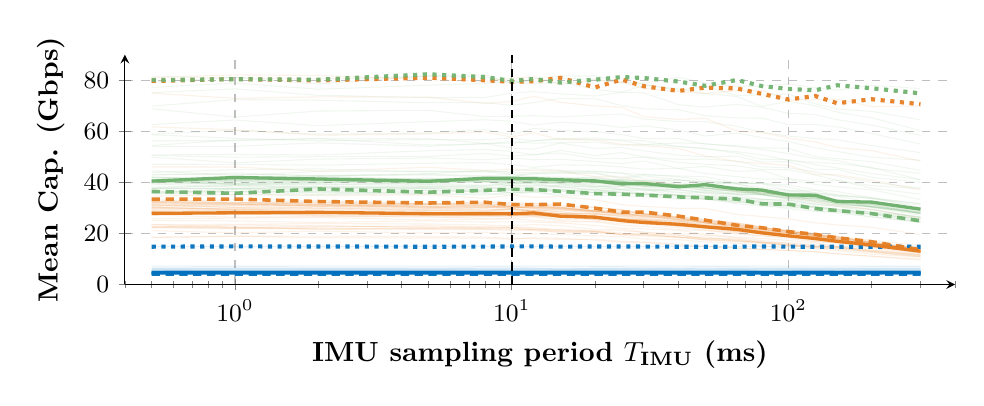
\begin{tikzpicture}
    \begin{axis}[width=\linewidth, height=4.5cm, xlabel={IMU sampling period $T_{\text{IMU}}$ (ms)}, ylabel={Mean Cap. (Gbps)}, xmin=0.4, xmax=400, ymin=0, ymax=90, every axis plot/.append style={mark=none}, xmode=log, log basis x=10,]
            \addplot[color=cb_blue, mark=none, opacity=0.10, line width=0.4pt, solid] coordinates {(0.5,14.89) (1,14.77) (2,14.88) (5,14.86) (8,14.9) (10,14.83) (12,14.86) (15,14.9) (20,14.85) (25,14.8) (30,14.83) (40,14.89) (50,14.81) (65,14.81) (80,14.91) (100,14.87) (125,14.82) (150,14.81) (200,14.83) (300,14.9)};
            \addplot[color=cb_blue, mark=none, opacity=0.10, line width=0.4pt, solid] coordinates {(0.5,7.18) (1,7.13) (2,7.17) (5,7.18) (8,7.15) (10,7.14) (12,7.18) (15,7.19) (20,7.15) (25,7.15) (30,7.2) (40,7.18) (50,7.13) (65,7.13) (80,7.18) (100,7.16) (125,7.17) (150,7.18) (200,7.14) (300,7.15)};
            \addplot[color=cb_blue, mark=none, opacity=0.10, line width=0.4pt, solid] coordinates {(0.5,6.46) (1,6.43) (2,6.43) (5,6.48) (8,6.45) (10,6.47) (12,6.43) (15,6.42) (20,6.43) (25,6.47) (30,6.43) (40,6.48) (50,6.44) (65,6.46) (80,6.46) (100,6.47) (125,6.43) (150,6.44) (200,6.44) (300,6.44)};
            \addplot[color=cb_blue, mark=none, opacity=0.10, line width=0.4pt, solid] coordinates {(0.5,6.14) (1,6.16) (2,6.15) (5,6.16) (8,6.13) (10,6.13) (12,6.17) (15,6.12) (20,6.16) (25,6.18) (30,6.13) (40,6.16) (50,6.12) (65,6.16) (80,6.18) (100,6.17) (125,6.18) (150,6.15) (200,6.14) (300,6.15)};
            \addplot[color=cb_blue, mark=none, opacity=0.10, line width=0.4pt, solid] coordinates {(0.5,5.88) (1,5.91) (2,5.92) (5,5.9) (8,5.91) (10,5.9) (12,5.88) (15,5.86) (20,5.88) (25,5.88) (30,5.86) (40,5.88) (50,5.9) (65,5.9) (80,5.91) (100,5.86) (125,5.89) (150,5.91) (200,5.87) (300,5.9)};
            \addplot[color=cb_blue, mark=none, opacity=0.10, line width=0.4pt, solid] coordinates {(0.5,5.66) (1,5.63) (2,5.65) (5,5.65) (8,5.64) (10,5.63) (12,5.62) (15,5.67) (20,5.67) (25,5.66) (30,5.61) (40,5.63) (50,5.61) (65,5.66) (80,5.63) (100,5.64) (125,5.65) (150,5.63) (200,5.65) (300,5.62)};
            \addplot[color=cb_blue, mark=none, opacity=0.10, line width=0.4pt, solid] coordinates {(0.5,5.5) (1,5.53) (2,5.53) (5,5.54) (8,5.53) (10,5.53) (12,5.52) (15,5.5) (20,5.49) (25,5.49) (30,5.51) (40,5.51) (50,5.53) (65,5.51) (80,5.49) (100,5.53) (125,5.5) (150,5.52) (200,5.51) (300,5.53)};
            \addplot[color=cb_blue, mark=none, opacity=0.10, line width=0.4pt, solid] coordinates {(0.5,5.38) (1,5.4) (2,5.38) (5,5.41) (8,5.38) (10,5.38) (12,5.41) (15,5.41) (20,5.38) (25,5.39) (30,5.41) (40,5.38) (50,5.42) (65,5.42) (80,5.41) (100,5.38) (125,5.39) (150,5.4) (200,5.42) (300,5.38)};
            \addplot[color=cb_blue, mark=none, opacity=0.10, line width=0.4pt, solid] coordinates {(0.5,5.28) (1,5.3) (2,5.31) (5,5.27) (8,5.3) (10,5.31) (12,5.32) (15,5.31) (20,5.3) (25,5.3) (30,5.29) (40,5.31) (50,5.31) (65,5.29) (80,5.3) (100,5.3) (125,5.31) (150,5.31) (200,5.28) (300,5.27)};
            \addplot[color=cb_blue, mark=none, opacity=0.10, line width=0.4pt, solid] coordinates {(0.5,5.2) (1,5.2) (2,5.23) (5,5.24) (8,5.23) (10,5.2) (12,5.21) (15,5.24) (20,5.24) (25,5.22) (30,5.19) (40,5.2) (50,5.22) (65,5.24) (80,5.24) (100,5.21) (125,5.21) (150,5.23) (200,5.23) (300,5.22)};
            \addplot[color=cb_blue, mark=none, opacity=0.10, line width=0.4pt, solid] coordinates {(0.5,5.18) (1,5.16) (2,5.17) (5,5.17) (8,5.17) (10,5.15) (12,5.2) (15,5.19) (20,5.17) (25,5.17) (30,5.18) (40,5.15) (50,5.18) (65,5.19) (80,5.18) (100,5.18) (125,5.16) (150,5.2) (200,5.15) (300,5.2)};
            \addplot[color=cb_blue, mark=none, opacity=0.10, line width=0.4pt, solid] coordinates {(0.5,5.12) (1,5.11) (2,5.12) (5,5.11) (8,5.12) (10,5.1) (12,5.13) (15,5.1) (20,5.12) (25,5.09) (30,5.12) (40,5.12) (50,5.12) (65,5.08) (80,5.13) (100,5.09) (125,5.11) (150,5.1) (200,5.13) (300,5.11)};
            \addplot[color=cb_blue, mark=none, opacity=0.10, line width=0.4pt, solid] coordinates {(0.5,5.06) (1,5.07) (2,5.05) (5,5.04) (8,5.05) (10,5.07) (12,5.06) (15,5.04) (20,5.05) (25,5.03) (30,5.06) (40,5.03) (50,5.06) (65,5.04) (80,5.03) (100,5.06) (125,5.05) (150,5.06) (200,5.06) (300,5.06)};
            \addplot[color=cb_blue, mark=none, opacity=0.10, line width=0.4pt, solid] coordinates {(0.5,4.96) (1,4.94) (2,4.94) (5,4.97) (8,4.95) (10,4.94) (12,4.94) (15,4.97) (20,4.97) (25,4.93) (30,4.97) (40,4.96) (50,4.97) (65,4.98) (80,4.94) (100,4.98) (125,4.96) (150,4.98) (200,4.98) (300,4.94)};
            \addplot[color=cb_blue, mark=none, opacity=0.10, line width=0.4pt, solid] coordinates {(0.5,4.95) (1,4.91) (2,4.9) (5,4.95) (8,4.93) (10,4.93) (12,4.95) (15,4.93) (20,4.92) (25,4.9) (30,4.91) (40,4.92) (50,4.93) (65,4.94) (80,4.93) (100,4.92) (125,4.93) (150,4.94) (200,4.93) (300,4.94)};
            \addplot[color=cb_blue, mark=none, opacity=0.10, line width=0.4pt, solid] coordinates {(0.5,4.89) (1,4.88) (2,4.86) (5,4.88) (8,4.86) (10,4.85) (12,4.85) (15,4.87) (20,4.88) (25,4.87) (30,4.84) (40,4.87) (50,4.87) (65,4.86) (80,4.88) (100,4.88) (125,4.85) (150,4.87) (200,4.88) (300,4.86)};
            \addplot[color=cb_blue, mark=none, opacity=0.10, line width=0.4pt, solid] coordinates {(0.5,4.82) (1,4.8) (2,4.8) (5,4.84) (8,4.83) (10,4.8) (12,4.83) (15,4.79) (20,4.82) (25,4.82) (30,4.83) (40,4.82) (50,4.82) (65,4.82) (80,4.83) (100,4.83) (125,4.8) (150,4.83) (200,4.84) (300,4.84)};
            \addplot[color=cb_blue, mark=none, opacity=0.10, line width=0.4pt, solid] coordinates {(0.5,4.76) (1,4.78) (2,4.76) (5,4.77) (8,4.79) (10,4.75) (12,4.75) (15,4.76) (20,4.76) (25,4.77) (30,4.79) (40,4.75) (50,4.79) (65,4.77) (80,4.76) (100,4.77) (125,4.77) (150,4.79) (200,4.75) (300,4.76)};
            \addplot[color=cb_blue, mark=none, opacity=0.10, line width=0.4pt, solid] coordinates {(0.5,4.75) (1,4.73) (2,4.74) (5,4.74) (8,4.73) (10,4.74) (12,4.74) (15,4.73) (20,4.75) (25,4.72) (30,4.73) (40,4.72) (50,4.71) (65,4.75) (80,4.72) (100,4.72) (125,4.72) (150,4.75) (200,4.75) (300,4.74)};
            \addplot[color=cb_blue, mark=none, opacity=0.10, line width=0.4pt, solid] coordinates {(0.5,4.68) (1,4.69) (2,4.68) (5,4.7) (8,4.68) (10,4.68) (12,4.69) (15,4.71) (20,4.69) (25,4.68) (30,4.68) (40,4.69) (50,4.7) (65,4.7) (80,4.68) (100,4.71) (125,4.72) (150,4.7) (200,4.68) (300,4.69)};
            \addplot[color=cb_blue, mark=none, opacity=0.10, line width=0.4pt, solid] coordinates {(0.5,4.67) (1,4.68) (2,4.67) (5,4.66) (8,4.65) (10,4.69) (12,4.66) (15,4.64) (20,4.67) (25,4.64) (30,4.65) (40,4.64) (50,4.67) (65,4.64) (80,4.67) (100,4.66) (125,4.66) (150,4.65) (200,4.68) (300,4.65)};
            \addplot[color=cb_blue, mark=none, opacity=0.10, line width=0.4pt, solid] coordinates {(0.5,4.61) (1,4.63) (2,4.66) (5,4.63) (8,4.62) (10,4.66) (12,4.62) (15,4.65) (20,4.63) (25,4.65) (30,4.64) (40,4.64) (50,4.65) (65,4.65) (80,4.64) (100,4.64) (125,4.65) (150,4.62) (200,4.66) (300,4.63)};
            \addplot[color=cb_blue, mark=none, opacity=0.10, line width=0.4pt, solid] coordinates {(0.5,4.62) (1,4.63) (2,4.64) (5,4.62) (8,4.63) (10,4.64) (12,4.62) (15,4.6) (20,4.6) (25,4.62) (30,4.61) (40,4.6) (50,4.62) (65,4.63) (80,4.6) (100,4.63) (125,4.64) (150,4.63) (200,4.61) (300,4.63)};
            \addplot[color=cb_blue, mark=none, opacity=0.10, line width=0.4pt, solid] coordinates {(0.5,4.61) (1,4.58) (2,4.62) (5,4.61) (8,4.6) (10,4.59) (12,4.6) (15,4.62) (20,4.62) (25,4.61) (30,4.59) (40,4.62) (50,4.62) (65,4.59) (80,4.59) (100,4.58) (125,4.58) (150,4.61) (200,4.62) (300,4.58)};
            \addplot[color=cb_blue, mark=none, opacity=0.10, line width=0.4pt, solid] coordinates {(0.5,4.56) (1,4.59) (2,4.58) (5,4.58) (8,4.6) (10,4.6) (12,4.58) (15,4.58) (20,4.59) (25,4.58) (30,4.58) (40,4.6) (50,4.6) (65,4.59) (80,4.57) (100,4.58) (125,4.6) (150,4.59) (200,4.59) (300,4.59)};
            \addplot[color=cb_blue, mark=none, opacity=0.10, line width=0.4pt, solid] coordinates {(0.5,4.57) (1,4.54) (2,4.57) (5,4.58) (8,4.57) (10,4.57) (12,4.56) (15,4.56) (20,4.56) (25,4.58) (30,4.56) (40,4.57) (50,4.56) (65,4.54) (80,4.54) (100,4.57) (125,4.56) (150,4.58) (200,4.55) (300,4.55)};
            \addplot[color=cb_blue, mark=none, opacity=0.10, line width=0.4pt, solid] coordinates {(0.5,4.53) (1,4.52) (2,4.55) (5,4.52) (8,4.53) (10,4.54) (12,4.52) (15,4.52) (20,4.52) (25,4.52) (30,4.54) (40,4.54) (50,4.52) (65,4.52) (80,4.55) (100,4.54) (125,4.55) (150,4.51) (200,4.53) (300,4.54)};
            \addplot[color=cb_blue, mark=none, opacity=0.10, line width=0.4pt, solid] coordinates {(0.5,4.51) (1,4.5) (2,4.51) (5,4.5) (8,4.5) (10,4.49) (12,4.53) (15,4.5) (20,4.5) (25,4.49) (30,4.51) (40,4.49) (50,4.51) (65,4.49) (80,4.49) (100,4.51) (125,4.49) (150,4.52) (200,4.5) (300,4.5)};
            \addplot[color=cb_blue, mark=none, opacity=0.10, line width=0.4pt, solid] coordinates {(0.5,4.48) (1,4.48) (2,4.47) (5,4.5) (8,4.47) (10,4.48) (12,4.5) (15,4.47) (20,4.48) (25,4.48) (30,4.48) (40,4.5) (50,4.47) (65,4.47) (80,4.46) (100,4.48) (125,4.5) (150,4.5) (200,4.47) (300,4.47)};
            \addplot[color=cb_blue, mark=none, opacity=0.10, line width=0.4pt, solid] coordinates {(0.5,4.46) (1,4.47) (2,4.45) (5,4.46) (8,4.46) (10,4.47) (12,4.47) (15,4.45) (20,4.47) (25,4.48) (30,4.46) (40,4.48) (50,4.48) (65,4.46) (80,4.44) (100,4.44) (125,4.44) (150,4.45) (200,4.46) (300,4.47)};
            \addplot[color=cb_blue, mark=none, opacity=0.10, line width=0.4pt, solid] coordinates {(0.5,4.42) (1,4.44) (2,4.43) (5,4.46) (8,4.45) (10,4.43) (12,4.43) (15,4.43) (20,4.45) (25,4.42) (30,4.42) (40,4.44) (50,4.42) (65,4.45) (80,4.45) (100,4.46) (125,4.42) (150,4.45) (200,4.42) (300,4.44)};
            \addplot[color=cb_blue, mark=none, opacity=0.10, line width=0.4pt, solid] coordinates {(0.5,4.42) (1,4.42) (2,4.41) (5,4.4) (8,4.43) (10,4.41) (12,4.42) (15,4.4) (20,4.39) (25,4.39) (30,4.43) (40,4.43) (50,4.41) (65,4.42) (80,4.39) (100,4.39) (125,4.41) (150,4.4) (200,4.42) (300,4.4)};
            \addplot[color=cb_blue, mark=none, opacity=0.10, line width=0.4pt, solid] coordinates {(0.5,4.38) (1,4.38) (2,4.39) (5,4.39) (8,4.38) (10,4.37) (12,4.38) (15,4.38) (20,4.38) (25,4.38) (30,4.36) (40,4.36) (50,4.37) (65,4.4) (80,4.37) (100,4.38) (125,4.4) (150,4.37) (200,4.37) (300,4.4)};
            \addplot[color=cb_blue, mark=none, opacity=0.10, line width=0.4pt, solid] coordinates {(0.5,4.35) (1,4.35) (2,4.34) (5,4.34) (8,4.36) (10,4.38) (12,4.35) (15,4.37) (20,4.35) (25,4.37) (30,4.36) (40,4.35) (50,4.37) (65,4.35) (80,4.35) (100,4.38) (125,4.34) (150,4.37) (200,4.34) (300,4.36)};
            \addplot[color=cb_blue, mark=none, opacity=0.10, line width=0.4pt, solid] coordinates {(0.5,4.35) (1,4.34) (2,4.32) (5,4.34) (8,4.35) (10,4.32) (12,4.34) (15,4.33) (20,4.34) (25,4.36) (30,4.32) (40,4.34) (50,4.31) (65,4.32) (80,4.34) (100,4.32) (125,4.35) (150,4.35) (200,4.35) (300,4.35)};
            \addplot[color=cb_blue, mark=none, opacity=0.10, line width=0.4pt, solid] coordinates {(0.5,4.33) (1,4.31) (2,4.32) (5,4.33) (8,4.29) (10,4.31) (12,4.33) (15,4.31) (20,4.29) (25,4.31) (30,4.32) (40,4.29) (50,4.29) (65,4.31) (80,4.32) (100,4.32) (125,4.32) (150,4.3) (200,4.32) (300,4.33)};
            \addplot[color=cb_blue, mark=none, opacity=0.10, line width=0.4pt, solid] coordinates {(0.5,4.31) (1,4.27) (2,4.3) (5,4.28) (8,4.3) (10,4.28) (12,4.28) (15,4.27) (20,4.27) (25,4.27) (30,4.29) (40,4.3) (50,4.3) (65,4.28) (80,4.29) (100,4.29) (125,4.28) (150,4.27) (200,4.29) (300,4.29)};
            \addplot[color=cb_blue, mark=none, opacity=0.10, line width=0.4pt, solid] coordinates {(0.5,4.25) (1,4.24) (2,4.25) (5,4.24) (8,4.25) (10,4.28) (12,4.28) (15,4.25) (20,4.27) (25,4.27) (30,4.25) (40,4.28) (50,4.26) (65,4.24) (80,4.25) (100,4.27) (125,4.26) (150,4.24) (200,4.27) (300,4.26)};
            \addplot[color=cb_blue, mark=none, opacity=0.10, line width=0.4pt, solid] coordinates {(0.5,4.25) (1,4.23) (2,4.24) (5,4.23) (8,4.22) (10,4.25) (12,4.25) (15,4.23) (20,4.26) (25,4.22) (30,4.26) (40,4.24) (50,4.26) (65,4.25) (80,4.25) (100,4.22) (125,4.25) (150,4.23) (200,4.25) (300,4.25)};
            \addplot[color=cb_blue, mark=none, opacity=0.10, line width=0.4pt, solid] coordinates {(0.5,4.22) (1,4.22) (2,4.23) (5,4.2) (8,4.21) (10,4.22) (12,4.23) (15,4.23) (20,4.2) (25,4.2) (30,4.23) (40,4.21) (50,4.23) (65,4.2) (80,4.2) (100,4.2) (125,4.23) (150,4.2) (200,4.22) (300,4.23)};
            \addplot[color=cb_blue, mark=none, opacity=0.10, line width=0.4pt, solid] coordinates {(0.5,4.2) (1,4.18) (2,4.18) (5,4.18) (8,4.19) (10,4.2) (12,4.18) (15,4.18) (20,4.18) (25,4.21) (30,4.22) (40,4.18) (50,4.2) (65,4.2) (80,4.21) (100,4.2) (125,4.19) (150,4.18) (200,4.21) (300,4.21)};
            \addplot[color=cb_blue, mark=none, opacity=0.10, line width=0.4pt, solid] coordinates {(0.5,4.18) (1,4.15) (2,4.16) (5,4.16) (8,4.16) (10,4.18) (12,4.15) (15,4.19) (20,4.19) (25,4.16) (30,4.18) (40,4.17) (50,4.18) (65,4.16) (80,4.17) (100,4.18) (125,4.17) (150,4.16) (200,4.17) (300,4.16)};
            \addplot[color=cb_blue, mark=none, opacity=0.10, line width=0.4pt, solid] coordinates {(0.5,4.13) (1,4.16) (2,4.16) (5,4.14) (8,4.17) (10,4.14) (12,4.14) (15,4.15) (20,4.17) (25,4.14) (30,4.17) (40,4.13) (50,4.15) (65,4.14) (80,4.16) (100,4.14) (125,4.17) (150,4.15) (200,4.17) (300,4.17)};
            \addplot[color=cb_blue, mark=none, opacity=0.10, line width=0.4pt, solid] coordinates {(0.5,4.12) (1,4.12) (2,4.12) (5,4.12) (8,4.15) (10,4.13) (12,4.14) (15,4.12) (20,4.15) (25,4.15) (30,4.15) (40,4.14) (50,4.12) (65,4.14) (80,4.14) (100,4.14) (125,4.12) (150,4.14) (200,4.13) (300,4.15)};
            \addplot[color=cb_blue, mark=none, opacity=0.10, line width=0.4pt, solid] coordinates {(0.5,4.11) (1,4.1) (2,4.13) (5,4.12) (8,4.13) (10,4.13) (12,4.13) (15,4.1) (20,4.1) (25,4.13) (30,4.1) (40,4.12) (50,4.11) (65,4.11) (80,4.13) (100,4.13) (125,4.12) (150,4.1) (200,4.12) (300,4.14)};
            \addplot[color=cb_blue, mark=none, opacity=0.10, line width=0.4pt, solid] coordinates {(0.5,4.09) (1,4.08) (2,4.12) (5,4.09) (8,4.1) (10,4.09) (12,4.1) (15,4.11) (20,4.1) (25,4.11) (30,4.09) (40,4.11) (50,4.11) (65,4.09) (80,4.1) (100,4.1) (125,4.1) (150,4.1) (200,4.11) (300,4.1)};
            \addplot[color=cb_blue, mark=none, opacity=0.10, line width=0.4pt, solid] coordinates {(0.5,4.09) (1,4.08) (2,4.09) (5,4.09) (8,4.09) (10,4.09) (12,4.07) (15,4.06) (20,4.1) (25,4.06) (30,4.09) (40,4.1) (50,4.1) (65,4.07) (80,4.08) (100,4.1) (125,4.1) (150,4.1) (200,4.08) (300,4.07)};
            \addplot[color=cb_blue, mark=none, opacity=0.10, line width=0.4pt, solid] coordinates {(0.5,4.08) (1,4.09) (2,4.08) (5,4.06) (8,4.08) (10,4.05) (12,4.05) (15,4.09) (20,4.08) (25,4.06) (30,4.05) (40,4.09) (50,4.06) (65,4.08) (80,4.07) (100,4.05) (125,4.08) (150,4.08) (200,4.05) (300,4.06)};
            \addplot[color=cb_blue, mark=none, opacity=0.10, line width=0.4pt, solid] coordinates {(0.5,4.04) (1,4.04) (2,4.06) (5,4.07) (8,4.04) (10,4.04) (12,4.07) (15,4.07) (20,4.06) (25,4.05) (30,4.05) (40,4.05) (50,4.07) (65,4.06) (80,4.05) (100,4.04) (125,4.07) (150,4.04) (200,4.07) (300,4.06)};
            \addplot[color=cb_blue, mark=none, opacity=0.10, line width=0.4pt, solid] coordinates {(0.5,4.02) (1,4.06) (2,4.05) (5,4.06) (8,4.04) (10,4.06) (12,4.06) (15,4.04) (20,4.05) (25,4.04) (30,4.03) (40,4.06) (50,4.04) (65,4.06) (80,4.03) (100,4.03) (125,4.05) (150,4.03) (200,4.03) (300,4.05)};
            \addplot[color=cb_orange, mark=none, opacity=0.10, line width=0.4pt, solid] coordinates {(0.5,81.11) (1,82.1) (2,81.85) (5,80.26) (8,79.54) (10,80.81) (12,81.35) (15,78.31) (20,80.22) (25,79.03) (30,76.77) (40,75.6) (50,74.79) (65,75.92) (80,76.09) (100,72.24) (125,72.34) (150,72.58) (200,69.72) (300,69.89)};
            \addplot[color=cb_orange, mark=none, opacity=0.10, line width=0.4pt, solid] coordinates {(0.5,74.9) (1,72.92) (2,73.47) (5,73.35) (8,70.92) (10,71.67) (12,73.75) (15,71.37) (20,69.91) (25,69.38) (30,65.71) (40,64.67) (50,65.05) (65,60.1) (80,59.49) (100,57.41) (125,55.8) (150,53.61) (200,52.41) (300,48.35)};
            \addplot[color=cb_orange, mark=none, opacity=0.10, line width=0.4pt, solid] coordinates {(0.5,61.71) (1,60.58) (2,58.47) (5,58.99) (8,59.77) (10,57.78) (12,59.43) (15,56.7) (20,56.63) (25,54.88) (30,54.38) (40,53.28) (50,50.34) (65,48.16) (80,47.39) (100,46.64) (125,43.09) (150,42.94) (200,40.8) (300,36.99)};
            \addplot[color=cb_orange, mark=none, opacity=0.10, line width=0.4pt, solid] coordinates {(0.5,46.0) (1,46.02) (2,44.4) (5,45.88) (8,44.71) (10,45.1) (12,44.58) (15,44.52) (20,42.18) (25,42.16) (30,40.39) (40,39.01) (50,38.76) (65,36.47) (80,36.04) (100,34.44) (125,32.35) (150,30.87) (200,29.52) (300,25.9)};
            \addplot[color=cb_orange, mark=none, opacity=0.10, line width=0.4pt, solid] coordinates {(0.5,34.59) (1,35.23) (2,34.8) (5,35.07) (8,33.8) (10,34.98) (12,34.15) (15,34.33) (20,33.14) (25,31.26) (30,30.61) (40,29.8) (50,29.75) (65,27.45) (80,26.63) (100,25.64) (125,24.16) (150,23.31) (200,22.41) (300,19.54)};
            \addplot[color=cb_orange, mark=none, opacity=0.10, line width=0.4pt, solid] coordinates {(0.5,28.05) (1,27.59) (2,28.29) (5,27.76) (8,26.95) (10,26.87) (12,27.25) (15,26.11) (20,26.49) (25,25.26) (30,25.27) (40,24.38) (50,22.66) (65,21.95) (80,21.65) (100,20.83) (125,19.3) (150,18.79) (200,17.33) (300,15.22)};
            \addplot[color=cb_orange, mark=none, opacity=0.10, line width=0.4pt, solid] coordinates {(0.5,22.31) (1,21.97) (2,21.77) (5,21.62) (8,21.64) (10,21.06) (12,21.49) (15,20.29) (20,20.6) (25,19.53) (30,18.96) (40,18.44) (50,17.52) (65,17.02) (80,16.43) (100,15.41) (125,14.95) (150,14.44) (200,13.56) (300,11.74)};
            \addplot[color=cb_orange, mark=none, opacity=0.10, line width=0.4pt, solid] coordinates {(0.5,18.38) (1,18.87) (2,18.93) (5,18.78) (8,18.56) (10,18.0) (12,17.96) (15,17.65) (20,17.75) (25,16.87) (30,16.66) (40,15.8) (50,15.1) (65,14.25) (80,13.77) (100,13.35) (125,12.8) (150,12.04) (200,10.98) (300,9.95)};
            \addplot[color=cb_orange, mark=none, opacity=0.10, line width=0.4pt, solid] coordinates {(0.5,18.53) (1,18.93) (2,18.29) (5,18.2) (8,18.16) (10,17.74) (12,18.32) (15,18.08) (20,17.34) (25,16.54) (30,16.45) (40,15.34) (50,14.78) (65,14.35) (80,13.7) (100,13.33) (125,12.75) (150,11.97) (200,11.13) (300,9.57)};
            \addplot[color=cb_orange, mark=none, opacity=0.10, line width=0.4pt, solid] coordinates {(0.5,21.09) (1,20.2) (2,20.9) (5,20.15) (8,20.48) (10,19.85) (12,19.85) (15,19.58) (20,19.07) (25,18.77) (30,17.84) (40,17.56) (50,16.63) (65,16.12) (80,15.23) (100,14.23) (125,14.03) (150,13.26) (200,11.9) (300,10.72)};
            \addplot[color=cb_orange, mark=none, opacity=0.10, line width=0.4pt, solid] coordinates {(0.5,22.62) (1,22.15) (2,22.75) (5,22.5) (8,22.19) (10,22.14) (12,21.48) (15,20.92) (20,20.63) (25,19.77) (30,19.99) (40,18.44) (50,18.53) (65,17.16) (80,16.55) (100,15.34) (125,14.86) (150,14.43) (200,12.81) (300,11.35)};
            \addplot[color=cb_orange, mark=none, opacity=0.10, line width=0.4pt, solid] coordinates {(0.5,23.55) (1,22.4) (2,22.39) (5,23.06) (8,22.33) (10,22.42) (12,21.79) (15,21.63) (20,20.97) (25,21.02) (30,20.52) (40,19.26) (50,18.02) (65,17.85) (80,16.43) (100,16.32) (125,15.15) (150,14.69) (200,13.37) (300,11.59)};
            \addplot[color=cb_orange, mark=none, opacity=0.10, line width=0.4pt, solid] coordinates {(0.5,22.2) (1,22.01) (2,21.8) (5,21.82) (8,21.7) (10,21.91) (12,21.01) (15,20.7) (20,20.34) (25,19.54) (30,19.45) (40,18.56) (50,17.71) (65,17.23) (80,16.37) (100,15.36) (125,14.41) (150,13.94) (200,12.98) (300,11.2)};
            \addplot[color=cb_orange, mark=none, opacity=0.10, line width=0.4pt, solid] coordinates {(0.5,22.88) (1,22.52) (2,21.6) (5,22.0) (8,21.87) (10,21.6) (12,21.49) (15,21.36) (20,20.9) (25,19.5) (30,19.35) (40,18.62) (50,17.42) (65,16.77) (80,16.15) (100,15.18) (125,14.51) (150,13.74) (200,12.46) (300,10.92)};
            \addplot[color=cb_orange, mark=none, opacity=0.10, line width=0.4pt, solid] coordinates {(0.5,22.46) (1,23.27) (2,23.06) (5,22.29) (8,22.65) (10,22.47) (12,22.29) (15,21.09) (20,20.84) (25,20.1) (30,19.65) (40,19.34) (50,18.03) (65,17.62) (80,16.82) (100,15.65) (125,14.65) (150,14.38) (200,12.84) (300,10.84)};
            \addplot[color=cb_orange, mark=none, opacity=0.10, line width=0.4pt, solid] coordinates {(0.5,23.41) (1,23.52) (2,23.88) (5,23.67) (8,23.31) (10,22.95) (12,23.44) (15,23.05) (20,21.53) (25,21.7) (30,20.33) (40,19.86) (50,19.26) (65,18.26) (80,17.26) (100,16.0) (125,15.48) (150,14.95) (200,13.11) (300,11.69)};
            \addplot[color=cb_orange, mark=none, opacity=0.10, line width=0.4pt, solid] coordinates {(0.5,25.13) (1,24.86) (2,24.28) (5,24.92) (8,24.44) (10,24.54) (12,24.49) (15,24.1) (20,23.11) (25,22.05) (30,21.79) (40,21.22) (50,19.63) (65,18.53) (80,18.01) (100,17.23) (125,16.21) (150,14.95) (200,14.11) (300,12.23)};
            \addplot[color=cb_orange, mark=none, opacity=0.10, line width=0.4pt, solid] coordinates {(0.5,25.76) (1,25.99) (2,26.28) (5,25.25) (8,25.55) (10,25.72) (12,25.12) (15,24.5) (20,24.53) (25,23.13) (30,22.8) (40,21.44) (50,21.14) (65,20.06) (80,19.14) (100,18.03) (125,16.66) (150,16.32) (200,14.65) (300,12.55)};
            \addplot[color=cb_orange, mark=none, opacity=0.10, line width=0.4pt, solid] coordinates {(0.5,27.15) (1,26.33) (2,26.62) (5,26.56) (8,25.79) (10,25.96) (12,26.5) (15,24.98) (20,24.69) (25,23.82) (30,23.76) (40,22.16) (50,21.38) (65,19.79) (80,18.94) (100,18.74) (125,16.88) (150,16.5) (200,14.78) (300,12.59)};
            \addplot[color=cb_orange, mark=none, opacity=0.10, line width=0.4pt, solid] coordinates {(0.5,28.24) (1,27.91) (2,26.86) (5,26.38) (8,26.48) (10,26.95) (12,26.73) (15,25.47) (20,25.86) (25,25.14) (30,23.86) (40,22.9) (50,21.9) (65,20.35) (80,19.99) (100,19.09) (125,17.32) (150,16.27) (200,14.78) (300,12.92)};
            \addplot[color=cb_orange, mark=none, opacity=0.10, line width=0.4pt, solid] coordinates {(0.5,27.48) (1,28.28) (2,27.05) (5,26.94) (8,26.96) (10,26.75) (12,27.17) (15,26.93) (20,25.22) (25,24.75) (30,24.66) (40,22.81) (50,22.1) (65,20.67) (80,20.16) (100,18.83) (125,17.72) (150,16.68) (200,14.99) (300,12.75)};
            \addplot[color=cb_orange, mark=none, opacity=0.10, line width=0.4pt, solid] coordinates {(0.5,28.81) (1,28.9) (2,27.84) (5,27.74) (8,27.87) (10,28.06) (12,27.16) (15,27.28) (20,26.62) (25,25.25) (30,25.06) (40,23.34) (50,22.75) (65,21.61) (80,20.41) (100,19.28) (125,17.96) (150,17.11) (200,15.38) (300,13.24)};
            \addplot[color=cb_orange, mark=none, opacity=0.10, line width=0.4pt, solid] coordinates {(0.5,28.1) (1,28.05) (2,27.67) (5,28.08) (8,28.05) (10,27.58) (12,28.04) (15,27.25) (20,26.79) (25,25.22) (30,24.15) (40,23.18) (50,22.38) (65,21.69) (80,20.22) (100,18.84) (125,18.23) (150,16.99) (200,15.72) (300,12.9)};
            \addplot[color=cb_orange, mark=none, opacity=0.10, line width=0.4pt, solid] coordinates {(0.5,28.37) (1,27.73) (2,27.99) (5,27.92) (8,28.24) (10,28.32) (12,27.57) (15,26.79) (20,26.21) (25,25.34) (30,24.13) (40,23.19) (50,22.6) (65,21.67) (80,20.62) (100,18.73) (125,18.32) (150,16.92) (200,15.58) (300,12.91)};
            \addplot[color=cb_orange, mark=none, opacity=0.10, line width=0.4pt, solid] coordinates {(0.5,28.21) (1,27.84) (2,28.5) (5,27.8) (8,28.35) (10,27.5) (12,26.81) (15,26.35) (20,25.7) (25,25.0) (30,24.56) (40,23.04) (50,22.48) (65,21.49) (80,20.6) (100,19.37) (125,17.62) (150,17.12) (200,15.16) (300,13.14)};
            \addplot[color=cb_orange, mark=none, opacity=0.10, line width=0.4pt, solid] coordinates {(0.5,28.82) (1,27.38) (2,28.03) (5,26.97) (8,26.88) (10,27.78) (12,27.39) (15,26.26) (20,26.02) (25,24.8) (30,24.31) (40,22.86) (50,22.23) (65,20.79) (80,20.09) (100,18.74) (125,17.93) (150,17.03) (200,14.76) (300,12.62)};
            \addplot[color=cb_orange, mark=none, opacity=0.10, line width=0.4pt, solid] coordinates {(0.5,28.54) (1,27.51) (2,27.34) (5,27.03) (8,27.03) (10,27.26) (12,27.48) (15,26.6) (20,25.39) (25,24.65) (30,24.84) (40,23.02) (50,22.64) (65,21.49) (80,20.4) (100,19.18) (125,17.45) (150,16.91) (200,14.77) (300,12.98)};
            \addplot[color=cb_orange, mark=none, opacity=0.10, line width=0.4pt, solid] coordinates {(0.5,28.04) (1,28.2) (2,28.4) (5,28.4) (8,27.51) (10,27.31) (12,26.98) (15,26.88) (20,25.56) (25,25.72) (30,24.87) (40,23.82) (50,22.9) (65,21.05) (80,20.06) (100,18.61) (125,17.81) (150,16.85) (200,15.28) (300,13.06)};
            \addplot[color=cb_orange, mark=none, opacity=0.10, line width=0.4pt, solid] coordinates {(0.5,28.69) (1,29.07) (2,28.14) (5,27.93) (8,27.83) (10,27.47) (12,27.84) (15,27.72) (20,26.52) (25,25.81) (30,24.44) (40,23.1) (50,23.12) (65,20.87) (80,19.8) (100,18.86) (125,18.22) (150,16.65) (200,14.96) (300,12.64)};
            \addplot[color=cb_orange, mark=none, opacity=0.10, line width=0.4pt, solid] coordinates {(0.5,29.71) (1,29.4) (2,29.67) (5,29.24) (8,28.45) (10,28.59) (12,27.87) (15,27.8) (20,27.43) (25,25.69) (30,25.15) (40,24.65) (50,23.47) (65,21.78) (80,20.99) (100,19.2) (125,18.07) (150,16.94) (200,15.39) (300,13.28)};
            \addplot[color=cb_orange, mark=none, opacity=0.10, line width=0.4pt, solid] coordinates {(0.5,30.43) (1,29.46) (2,30.33) (5,29.85) (8,28.96) (10,29.84) (12,28.51) (15,27.71) (20,27.66) (25,26.53) (30,25.55) (40,25.1) (50,23.03) (65,22.13) (80,20.74) (100,19.89) (125,18.63) (150,17.16) (200,15.64) (300,12.99)};
            \addplot[color=cb_orange, mark=none, opacity=0.10, line width=0.4pt, solid] coordinates {(0.5,31.66) (1,31.56) (2,30.86) (5,30.36) (8,30.37) (10,30.59) (12,30.17) (15,29.51) (20,28.44) (25,27.91) (30,27.08) (40,26.14) (50,24.11) (65,22.56) (80,21.42) (100,20.42) (125,18.92) (150,17.86) (200,16.18) (300,13.81)};
            \addplot[color=cb_orange, mark=none, opacity=0.10, line width=0.4pt, solid] coordinates {(0.5,32.12) (1,31.37) (2,30.69) (5,31.37) (8,31.44) (10,30.42) (12,30.01) (15,30.27) (20,28.62) (25,27.66) (30,27.29) (40,26.12) (50,24.19) (65,23.3) (80,22.36) (100,20.82) (125,19.32) (150,18.75) (200,16.32) (300,13.69)};
            \addplot[color=cb_orange, mark=none, opacity=0.10, line width=0.4pt, solid] coordinates {(0.5,31.31) (1,31.27) (2,32.17) (5,30.67) (8,30.31) (10,30.96) (12,30.41) (15,29.56) (20,28.69) (25,27.54) (30,27.58) (40,26.44) (50,24.96) (65,23.99) (80,22.36) (100,20.95) (125,19.36) (150,18.1) (200,16.86) (300,13.9)};
            \addplot[color=cb_orange, mark=none, opacity=0.10, line width=0.4pt, solid] coordinates {(0.5,32.55) (1,32.07) (2,31.35) (5,30.48) (8,30.3) (10,30.14) (12,30.15) (15,30.17) (20,28.75) (25,28.25) (30,27.79) (40,25.46) (50,24.63) (65,23.08) (80,21.54) (100,20.62) (125,19.63) (150,18.64) (200,16.66) (300,13.95)};
            \addplot[color=cb_orange, mark=none, opacity=0.10, line width=0.4pt, solid] coordinates {(0.5,32.32) (1,31.6) (2,30.61) (5,31.2) (8,31.11) (10,29.94) (12,31.08) (15,30.26) (20,28.96) (25,27.33) (30,27.03) (40,25.35) (50,24.85) (65,23.7) (80,21.83) (100,20.93) (125,19.03) (150,18.61) (200,16.45) (300,13.92)};
            \addplot[color=cb_orange, mark=none, opacity=0.10, line width=0.4pt, solid] coordinates {(0.5,32.06) (1,31.52) (2,31.63) (5,30.63) (8,31.25) (10,30.52) (12,29.8) (15,29.8) (20,29.08) (25,27.49) (30,26.73) (40,26.12) (50,24.14) (65,22.44) (80,21.83) (100,20.35) (125,19.27) (150,17.97) (200,16.15) (300,13.78)};
            \addplot[color=cb_orange, mark=none, opacity=0.10, line width=0.4pt, solid] coordinates {(0.5,31.31) (1,30.31) (2,31.12) (5,30.11) (8,30.23) (10,29.83) (12,29.05) (15,29.63) (20,28.14) (25,27.32) (30,26.05) (40,24.72) (50,24.23) (65,21.96) (80,20.87) (100,19.87) (125,18.85) (150,17.25) (200,15.67) (300,13.11)};
            \addplot[color=cb_orange, mark=none, opacity=0.10, line width=0.4pt, solid] coordinates {(0.5,30.24) (1,29.04) (2,29.19) (5,29.05) (8,28.8) (10,29.57) (12,28.97) (15,28.52) (20,26.71) (25,25.78) (30,25.27) (40,24.87) (50,22.84) (65,21.94) (80,20.3) (100,19.22) (125,18.18) (150,16.99) (200,15.58) (300,12.82)};
            \addplot[color=cb_orange, mark=none, opacity=0.10, line width=0.4pt, solid] coordinates {(0.5,29.26) (1,29.84) (2,28.36) (5,28.31) (8,28.23) (10,28.17) (12,28.22) (15,27.8) (20,26.37) (25,25.87) (30,25.25) (40,23.39) (50,22.28) (65,21.43) (80,20.08) (100,18.66) (125,17.85) (150,16.83) (200,15.02) (300,12.35)};
            \addplot[color=cb_orange, mark=none, opacity=0.10, line width=0.4pt, solid] coordinates {(0.5,30.25) (1,29.38) (2,28.72) (5,28.87) (8,28.54) (10,29.36) (12,28.73) (15,27.79) (20,26.79) (25,25.93) (30,25.16) (40,23.42) (50,22.98) (65,22.07) (80,20.39) (100,19.48) (125,18.05) (150,16.7) (200,14.91) (300,12.52)};
            \addplot[color=cb_orange, mark=none, opacity=0.10, line width=0.4pt, solid] coordinates {(0.5,29.66) (1,30.07) (2,29.88) (5,29.18) (8,29.7) (10,29.1) (12,28.8) (15,27.64) (20,27.78) (25,26.99) (30,25.67) (40,23.86) (50,22.79) (65,22.31) (80,20.97) (100,19.39) (125,17.88) (150,16.96) (200,15.33) (300,12.59)};
            \addplot[color=cb_orange, mark=none, opacity=0.10, line width=0.4pt, solid] coordinates {(0.5,30.11) (1,30.93) (2,30.6) (5,30.39) (8,29.2) (10,29.36) (12,28.95) (15,29.21) (20,27.86) (25,26.6) (30,26.42) (40,25.28) (50,23.49) (65,22.12) (80,21.7) (100,19.4) (125,18.54) (150,17.59) (200,15.29) (300,12.56)};
            \addplot[color=cb_orange, mark=none, opacity=0.10, line width=0.4pt, solid] coordinates {(0.5,31.14) (1,30.17) (2,29.91) (5,29.77) (8,30.02) (10,30.48) (12,29.57) (15,28.39) (20,27.5) (25,27.01) (30,26.98) (40,25.39) (50,24.27) (65,22.51) (80,21.63) (100,20.17) (125,18.97) (150,17.61) (200,15.6) (300,13.01)};
            \addplot[color=cb_orange, mark=none, opacity=0.10, line width=0.4pt, solid] coordinates {(0.5,30.85) (1,31.6) (2,31.12) (5,30.06) (8,30.77) (10,30.4) (12,29.96) (15,29.06) (20,28.59) (25,28.07) (30,26.63) (40,25.47) (50,23.99) (65,22.92) (80,21.09) (100,20.11) (125,18.75) (150,17.26) (200,15.76) (300,13.07)};
            \addplot[color=cb_orange, mark=none, opacity=0.10, line width=0.4pt, solid] coordinates {(0.5,30.74) (1,30.97) (2,31.27) (5,31.33) (8,30.75) (10,29.8) (12,30.77) (15,30.21) (20,28.46) (25,27.89) (30,26.47) (40,26.0) (50,24.06) (65,23.21) (80,21.61) (100,20.13) (125,19.09) (150,17.64) (200,15.5) (300,13.16)};
            \addplot[color=cb_orange, mark=none, opacity=0.10, line width=0.4pt, solid] coordinates {(0.5,31.91) (1,32.26) (2,31.41) (5,31.69) (8,31.63) (10,30.76) (12,31.17) (15,29.82) (20,28.91) (25,28.72) (30,27.5) (40,25.73) (50,24.67) (65,23.42) (80,22.11) (100,21.1) (125,19.52) (150,18.09) (200,15.83) (300,13.16)};
            \addplot[color=cb_orange, mark=none, opacity=0.10, line width=0.4pt, solid] coordinates {(0.5,33.26) (1,32.03) (2,32.22) (5,31.56) (8,30.83) (10,32.02) (12,30.59) (15,29.85) (20,28.82) (25,29.07) (30,27.57) (40,26.51) (50,25.58) (65,23.85) (80,22.51) (100,20.6) (125,19.84) (150,17.94) (200,16.6) (300,13.56)};
            \addplot[color=cb_orange, mark=none, opacity=0.10, line width=0.4pt, solid] coordinates {(0.5,32.72) (1,31.89) (2,32.54) (5,31.41) (8,32.41) (10,31.1) (12,31.84) (15,30.93) (20,30.19) (25,29.33) (30,27.62) (40,26.68) (50,25.06) (65,24.28) (80,22.54) (100,20.74) (125,19.37) (150,18.34) (200,16.23) (300,13.28)};
            \addplot[color=cb_orange, mark=none, opacity=0.10, line width=0.4pt, solid] coordinates {(0.5,32.37) (1,33.19) (2,32.93) (5,31.6) (8,32.06) (10,32.05) (12,31.76) (15,30.37) (20,30.21) (25,29.35) (30,27.73) (40,26.34) (50,25.31) (65,23.23) (80,22.13) (100,21.33) (125,20.03) (150,18.53) (200,16.4) (300,13.69)};
            \addplot[color=cb_green, mark=none, opacity=0.10, line width=0.4pt, solid] coordinates {(0.5,81.33) (1,80.94) (2,80.45) (5,81.53) (8,81.28) (10,79.58) (12,79.29) (15,80.75) (20,80.41) (25,78.97) (30,78.78) (40,81.18) (50,78.86) (65,77.64) (80,77.65) (100,78.59) (125,76.98) (150,76.09) (200,78.03) (300,76.71)};
            \addplot[color=cb_green, mark=none, opacity=0.10, line width=0.4pt, solid] coordinates {(0.5,79.28) (1,81.09) (2,78.54) (5,81.77) (8,82.15) (10,78.57) (12,80.58) (15,81.69) (20,81.65) (25,79.39) (30,78.43) (40,76.03) (50,77.54) (65,74.02) (80,74.25) (100,74.57) (125,70.79) (150,68.76) (200,67.82) (300,64.48)};
            \addplot[color=cb_green, mark=none, opacity=0.10, line width=0.4pt, solid] coordinates {(0.5,77.23) (1,78.9) (2,76.47) (5,78.06) (8,78.78) (10,79.52) (12,78.51) (15,79.34) (20,76.46) (25,75.27) (30,78.01) (40,76.65) (50,74.82) (65,73.63) (80,69.77) (100,71.69) (125,70.01) (150,67.48) (200,65.29) (300,60.24)};
            \addplot[color=cb_green, mark=none, opacity=0.10, line width=0.4pt, solid] coordinates {(0.5,75.14) (1,76.62) (2,74.09) (5,73.23) (8,73.21) (10,74.98) (12,75.51) (15,74.69) (20,73.82) (25,75.25) (30,75.07) (40,70.42) (50,69.48) (65,70.57) (80,69.42) (100,67.01) (125,66.5) (150,64.55) (200,62.42) (300,58.37)};
            \addplot[color=cb_green, mark=none, opacity=0.10, line width=0.4pt, solid] coordinates {(0.5,69.86) (1,72.41) (2,72.16) (5,71.21) (8,71.2) (10,70.17) (12,71.24) (15,72.88) (20,72.78) (25,70.01) (30,68.79) (40,68.45) (50,66.1) (65,65.27) (80,65.19) (100,62.58) (125,62.65) (150,61.71) (200,59.13) (300,55.01)};
            \addplot[color=cb_green, mark=none, opacity=0.10, line width=0.4pt, solid] coordinates {(0.5,68.83) (1,65.55) (2,67.92) (5,68.23) (8,65.76) (10,65.93) (12,66.11) (15,65.65) (20,66.3) (25,66.74) (30,64.79) (40,63.81) (50,63.76) (65,61.97) (80,59.67) (100,58.15) (125,57.17) (150,56.71) (200,54.38) (300,51.64)};
            \addplot[color=cb_green, mark=none, opacity=0.10, line width=0.4pt, solid] coordinates {(0.5,62.64) (1,64.4) (2,62.21) (5,63.76) (8,64.48) (10,63.97) (12,62.44) (15,63.58) (20,62.81) (25,61.45) (30,62.2) (40,60.5) (50,58.15) (65,59.3) (80,57.55) (100,55.94) (125,53.55) (150,52.1) (200,49.85) (300,48.68)};
            \addplot[color=cb_green, mark=none, opacity=0.10, line width=0.4pt, solid] coordinates {(0.5,58.91) (1,60.43) (2,58.85) (5,59.33) (8,60.66) (10,58.64) (12,61.14) (15,60.3) (20,59.8) (25,58.69) (30,57.14) (40,57.19) (50,54.91) (65,54.31) (80,53.48) (100,53.34) (125,50.01) (150,49.3) (200,48.07) (300,44.68)};
            \addplot[color=cb_green, mark=none, opacity=0.10, line width=0.4pt, solid] coordinates {(0.5,58.63) (1,57.26) (2,56.28) (5,56.74) (8,56.68) (10,57.39) (12,56.3) (15,57.03) (20,57.36) (25,56.29) (30,54.84) (40,55.42) (50,55.22) (65,54.01) (80,52.83) (100,51.27) (125,49.33) (150,48.53) (200,45.54) (300,43.55)};
            \addplot[color=cb_green, mark=none, opacity=0.10, line width=0.4pt, solid] coordinates {(0.5,56.31) (1,56.29) (2,57.14) (5,57.16) (8,55.24) (10,55.39) (12,56.18) (15,57.12) (20,56.65) (25,56.63) (30,56.29) (40,53.94) (50,53.27) (65,51.99) (80,50.75) (100,48.59) (125,47.76) (150,47.43) (200,45.81) (300,41.04)};
            \addplot[color=cb_green, mark=none, opacity=0.10, line width=0.4pt, solid] coordinates {(0.5,54.45) (1,56.64) (2,57.06) (5,54.64) (8,55.1) (10,55.92) (12,55.35) (15,55.51) (20,55.77) (25,54.55) (30,54.82) (40,54.09) (50,53.19) (65,51.39) (80,49.07) (100,48.89) (125,46.92) (150,45.61) (200,43.44) (300,41.02)};
            \addplot[color=cb_green, mark=none, opacity=0.10, line width=0.4pt, solid] coordinates {(0.5,54.04) (1,54.11) (2,55.46) (5,54.15) (8,55.13) (10,53.44) (12,53.0) (15,55.39) (20,53.26) (25,53.64) (30,52.32) (40,50.65) (50,50.02) (65,50.25) (80,47.96) (100,48.11) (125,45.03) (150,45.0) (200,41.99) (300,39.98)};
            \addplot[color=cb_green, mark=none, opacity=0.10, line width=0.4pt, solid] coordinates {(0.5,50.75) (1,50.92) (2,50.72) (5,52.4) (8,52.86) (10,52.13) (12,50.73) (15,52.49) (20,50.46) (25,51.64) (30,49.97) (40,48.98) (50,49.1) (65,48.31) (80,46.06) (100,45.68) (125,44.09) (150,42.41) (200,39.97) (300,37.82)};
            \addplot[color=cb_green, mark=none, opacity=0.10, line width=0.4pt, solid] coordinates {(0.5,50.53) (1,49.84) (2,50.06) (5,50.18) (8,51.32) (10,50.29) (12,50.86) (15,51.45) (20,49.29) (25,49.26) (30,49.89) (40,47.8) (50,47.09) (65,46.47) (80,45.02) (100,44.92) (125,42.85) (150,40.77) (200,38.7) (300,37.54)};
            \addplot[color=cb_green, mark=none, opacity=0.10, line width=0.4pt, solid] coordinates {(0.5,49.84) (1,47.67) (2,49.1) (5,49.58) (8,48.86) (10,49.52) (12,48.85) (15,49.03) (20,48.14) (25,47.36) (30,48.33) (40,45.5) (50,46.23) (65,44.29) (80,44.63) (100,41.48) (125,40.24) (150,40.9) (200,37.67) (300,35.42)};
            \addplot[color=cb_green, mark=none, opacity=0.10, line width=0.4pt, solid] coordinates {(0.5,47.1) (1,47.04) (2,46.73) (5,47.47) (8,47.74) (10,46.99) (12,45.87) (15,46.86) (20,46.68) (25,46.02) (30,45.15) (40,45.5) (50,43.45) (65,42.23) (80,41.27) (100,41.21) (125,39.17) (150,38.31) (200,37.08) (300,33.27)};
            \addplot[color=cb_green, mark=none, opacity=0.10, line width=0.4pt, solid] coordinates {(0.5,43.84) (1,44.93) (2,45.26) (5,44.11) (8,44.08) (10,44.43) (12,45.33) (15,44.75) (20,44.35) (25,43.57) (30,43.05) (40,42.48) (50,42.21) (65,39.7) (80,39.6) (100,38.97) (125,37.11) (150,36.43) (200,33.96) (300,31.63)};
            \addplot[color=cb_green, mark=none, opacity=0.10, line width=0.4pt, solid] coordinates {(0.5,43.1) (1,43.16) (2,42.66) (5,43.4) (8,44.62) (10,43.73) (12,43.86) (15,44.16) (20,44.15) (25,43.65) (30,41.36) (40,40.73) (50,40.24) (65,39.77) (80,39.57) (100,38.13) (125,35.84) (150,34.7) (200,33.74) (300,31.61)};
            \addplot[color=cb_green, mark=none, opacity=0.10, line width=0.4pt, solid] coordinates {(0.5,44.5) (1,42.64) (2,44.24) (5,44.35) (8,44.32) (10,43.12) (12,43.23) (15,43.56) (20,43.61) (25,41.9) (30,43.1) (40,42.2) (50,40.76) (65,39.75) (80,39.54) (100,36.66) (125,36.8) (150,35.11) (200,33.6) (300,30.99)};
            \addplot[color=cb_green, mark=none, opacity=0.10, line width=0.4pt, solid] coordinates {(0.5,42.84) (1,43.66) (2,42.49) (5,42.9) (8,42.16) (10,42.27) (12,43.52) (15,43.84) (20,43.59) (25,41.34) (30,42.59) (40,41.09) (50,39.84) (65,39.33) (80,37.89) (100,36.94) (125,35.92) (150,35.06) (200,33.98) (300,30.08)};
            \addplot[color=cb_green, mark=none, opacity=0.10, line width=0.4pt, solid] coordinates {(0.5,41.93) (1,42.02) (2,42.49) (5,43.2) (8,42.53) (10,43.09) (12,42.2) (15,41.98) (20,41.69) (25,40.97) (30,40.46) (40,40.96) (50,40.0) (65,39.43) (80,37.03) (100,36.54) (125,35.5) (150,34.58) (200,32.08) (300,29.89)};
            \addplot[color=cb_green, mark=none, opacity=0.10, line width=0.4pt, solid] coordinates {(0.5,40.13) (1,40.45) (2,40.78) (5,41.7) (8,40.48) (10,41.76) (12,41.91) (15,41.43) (20,41.49) (25,40.55) (30,39.06) (40,38.36) (50,38.81) (65,37.62) (80,35.4) (100,35.94) (125,34.91) (150,33.23) (200,32.03) (300,28.39)};
            \addplot[color=cb_green, mark=none, opacity=0.10, line width=0.4pt, solid] coordinates {(0.5,41.01) (1,39.39) (2,39.74) (5,41.23) (8,40.49) (10,40.81) (12,40.38) (15,41.01) (20,39.66) (25,38.88) (30,39.62) (40,39.04) (50,37.52) (65,36.49) (80,35.31) (100,35.34) (125,34.44) (150,33.04) (200,30.48) (300,28.43)};
            \addplot[color=cb_green, mark=none, opacity=0.10, line width=0.4pt, solid] coordinates {(0.5,39.63) (1,41.07) (2,40.94) (5,40.13) (8,40.49) (10,40.03) (12,40.74) (15,40.5) (20,40.76) (25,40.19) (30,38.98) (40,39.32) (50,37.61) (65,37.51) (80,36.36) (100,34.48) (125,34.27) (150,33.0) (200,31.72) (300,28.01)};
            \addplot[color=cb_green, mark=none, opacity=0.10, line width=0.4pt, solid] coordinates {(0.5,40.64) (1,39.37) (2,39.63) (5,40.12) (8,41.26) (10,40.72) (12,39.89) (15,39.66) (20,40.72) (25,40.13) (30,38.8) (40,37.81) (50,38.32) (65,37.42) (80,36.35) (100,35.11) (125,32.73) (150,31.9) (200,31.09) (300,28.13)};
            \addplot[color=cb_green, mark=none, opacity=0.10, line width=0.4pt, solid] coordinates {(0.5,40.94) (1,41.44) (2,41.12) (5,41.36) (8,41.79) (10,41.9) (12,41.58) (15,41.94) (20,40.66) (25,40.48) (30,39.89) (40,39.15) (50,38.73) (65,38.27) (80,36.59) (100,35.46) (125,34.53) (150,32.9) (200,31.29) (300,29.93)};
            \addplot[color=cb_green, mark=none, opacity=0.10, line width=0.4pt, solid] coordinates {(0.5,42.0) (1,41.03) (2,42.44) (5,41.11) (8,41.81) (10,40.67) (12,41.4) (15,41.09) (20,40.38) (25,41.15) (30,40.7) (40,39.95) (50,38.59) (65,38.13) (80,36.62) (100,35.41) (125,33.96) (150,33.07) (200,31.77) (300,29.78)};
            \addplot[color=cb_green, mark=none, opacity=0.10, line width=0.4pt, solid] coordinates {(0.5,42.11) (1,40.61) (2,42.09) (5,41.03) (8,41.15) (10,41.3) (12,41.4) (15,41.32) (20,42.09) (25,40.33) (30,40.8) (40,39.14) (50,39.27) (65,37.24) (80,36.5) (100,35.72) (125,33.86) (150,32.94) (200,31.96) (300,29.85)};
            \addplot[color=cb_green, mark=none, opacity=0.10, line width=0.4pt, solid] coordinates {(0.5,40.83) (1,40.25) (2,40.81) (5,39.63) (8,41.05) (10,41.21) (12,39.77) (15,41.02) (20,41.15) (25,40.42) (30,39.54) (40,38.87) (50,37.82) (65,36.49) (80,35.29) (100,34.18) (125,33.7) (150,33.24) (200,30.59) (300,28.93)};
            \addplot[color=cb_green, mark=none, opacity=0.10, line width=0.4pt, solid] coordinates {(0.5,40.27) (1,39.13) (2,38.9) (5,39.92) (8,40.33) (10,38.54) (12,38.51) (15,40.33) (20,38.4) (25,38.56) (30,38.29) (40,36.84) (50,36.35) (65,35.21) (80,35.28) (100,33.35) (125,32.29) (150,31.11) (200,30.53) (300,27.86)};
            \addplot[color=cb_green, mark=none, opacity=0.10, line width=0.4pt, solid] coordinates {(0.5,37.66) (1,38.83) (2,37.93) (5,37.57) (8,37.55) (10,38.8) (12,38.87) (15,38.21) (20,37.17) (25,38.31) (30,37.46) (40,35.8) (50,36.11) (65,35.2) (80,33.31) (100,32.99) (125,31.44) (150,30.53) (200,29.25) (300,26.2)};
            \addplot[color=cb_green, mark=none, opacity=0.10, line width=0.4pt, solid] coordinates {(0.5,37.61) (1,37.47) (2,37.59) (5,38.34) (8,37.98) (10,37.64) (12,37.26) (15,38.93) (20,37.88) (25,37.33) (30,37.69) (40,36.18) (50,34.92) (65,33.55) (80,33.51) (100,32.34) (125,31.24) (150,30.58) (200,28.38) (300,26.2)};
            \addplot[color=cb_green, mark=none, opacity=0.10, line width=0.4pt, solid] coordinates {(0.5,39.34) (1,38.23) (2,37.91) (5,38.18) (8,38.55) (10,38.7) (12,38.11) (15,39.02) (20,39.06) (25,36.98) (30,36.69) (40,37.15) (50,35.71) (65,34.29) (80,33.24) (100,33.02) (125,31.7) (150,31.14) (200,29.31) (300,26.44)};
            \addplot[color=cb_green, mark=none, opacity=0.10, line width=0.4pt, solid] coordinates {(0.5,40.11) (1,39.09) (2,39.21) (5,39.26) (8,38.89) (10,39.23) (12,39.71) (15,39.39) (20,38.32) (25,39.24) (30,38.91) (40,38.12) (50,36.87) (65,35.41) (80,35.11) (100,33.49) (125,33.01) (150,31.71) (200,30.6) (300,28.24)};
            \addplot[color=cb_green, mark=none, opacity=0.10, line width=0.4pt, solid] coordinates {(0.5,39.42) (1,39.47) (2,40.67) (5,40.02) (8,40.78) (10,39.59) (12,40.76) (15,39.59) (20,39.85) (25,40.47) (30,38.19) (40,38.07) (50,36.8) (65,36.91) (80,35.41) (100,34.79) (125,33.29) (150,32.05) (200,30.24) (300,27.91)};
            \addplot[color=cb_green, mark=none, opacity=0.10, line width=0.4pt, solid] coordinates {(0.5,40.23) (1,41.51) (2,41.01) (5,40.69) (8,40.88) (10,40.39) (12,40.95) (15,39.92) (20,40.4) (25,39.33) (30,39.68) (40,38.98) (50,37.8) (65,36.23) (80,35.69) (100,35.42) (125,34.22) (150,32.85) (200,31.35) (300,27.71)};
            \addplot[color=cb_green, mark=none, opacity=0.10, line width=0.4pt, solid] coordinates {(0.5,41.31) (1,41.94) (2,40.25) (5,41.09) (8,40.54) (10,40.37) (12,42.24) (15,40.87) (20,40.32) (25,40.91) (30,40.12) (40,38.81) (50,37.48) (65,37.17) (80,35.65) (100,34.91) (125,34.08) (150,32.51) (200,31.44) (300,29.22)};
            \addplot[color=cb_green, mark=none, opacity=0.10, line width=0.4pt, solid] coordinates {(0.5,40.08) (1,41.18) (2,41.28) (5,40.71) (8,40.14) (10,40.79) (12,40.34) (15,40.04) (20,40.32) (25,40.12) (30,38.5) (40,37.78) (50,38.07) (65,36.16) (80,35.2) (100,33.85) (125,33.86) (150,32.5) (200,31.07) (300,27.83)};
            \addplot[color=cb_green, mark=none, opacity=0.10, line width=0.4pt, solid] coordinates {(0.5,40.94) (1,40.58) (2,39.94) (5,41.01) (8,41.14) (10,40.73) (12,40.34) (15,39.72) (20,40.67) (25,40.63) (30,38.39) (40,38.89) (50,36.83) (65,35.81) (80,36.15) (100,34.09) (125,33.89) (150,31.5) (200,30.54) (300,27.85)};
            \addplot[color=cb_green, mark=none, opacity=0.10, line width=0.4pt, solid] coordinates {(0.5,40.4) (1,39.73) (2,40.07) (5,39.31) (8,40.19) (10,39.83) (12,39.84) (15,40.02) (20,39.41) (25,39.38) (30,38.94) (40,38.72) (50,37.83) (65,36.94) (80,35.97) (100,34.68) (125,33.29) (150,32.48) (200,30.34) (300,27.67)};
            \addplot[color=cb_green, mark=none, opacity=0.10, line width=0.4pt, solid] coordinates {(0.5,41.04) (1,40.83) (2,40.57) (5,40.33) (8,40.15) (10,39.5) (12,40.18) (15,40.39) (20,40.5) (25,40.17) (30,38.69) (40,38.47) (50,38.47) (65,37.26) (80,35.3) (100,33.86) (125,33.65) (150,31.43) (200,30.43) (300,27.95)};
            \addplot[color=cb_green, mark=none, opacity=0.10, line width=0.4pt, solid] coordinates {(0.5,38.13) (1,38.73) (2,38.31) (5,38.85) (8,38.62) (10,39.93) (12,39.31) (15,38.19) (20,38.38) (25,38.34) (30,37.07) (40,37.43) (50,35.83) (65,35.45) (80,35.12) (100,33.79) (125,32.69) (150,31.79) (200,30.2) (300,27.12)};
            \addplot[color=cb_green, mark=none, opacity=0.10, line width=0.4pt, solid] coordinates {(0.5,37.58) (1,37.54) (2,38.3) (5,38.07) (8,38.17) (10,36.73) (12,36.71) (15,38.34) (20,36.67) (25,37.34) (30,37.14) (40,34.98) (50,34.73) (65,34.44) (80,32.24) (100,32.17) (125,30.18) (150,29.3) (200,28.37) (300,26.5)};
            \addplot[color=cb_green, mark=none, opacity=0.10, line width=0.4pt, solid] coordinates {(0.5,35.6) (1,36.36) (2,35.28) (5,36.76) (8,36.78) (10,35.82) (12,36.53) (15,36.89) (20,36.04) (25,36.27) (30,35.1) (40,35.01) (50,33.36) (65,33.1) (80,31.97) (100,30.05) (125,30.14) (150,28.74) (200,27.51) (300,24.34)};
            \addplot[color=cb_green, mark=none, opacity=0.10, line width=0.4pt, solid] coordinates {(0.5,35.51) (1,35.21) (2,35.07) (5,35.62) (8,35.03) (10,36.05) (12,36.21) (15,34.72) (20,34.95) (25,34.69) (30,34.26) (40,33.85) (50,33.34) (65,32.16) (80,31.15) (100,29.66) (125,28.59) (150,28.61) (200,26.35) (300,24.56)};
            \addplot[color=cb_green, mark=none, opacity=0.10, line width=0.4pt, solid] coordinates {(0.5,36.6) (1,36.25) (2,36.29) (5,35.26) (8,35.54) (10,35.02) (12,36.17) (15,35.32) (20,36.1) (25,35.36) (30,35.39) (40,33.36) (50,33.58) (65,31.6) (80,30.64) (100,30.67) (125,28.84) (150,27.89) (200,26.62) (300,24.2)};
            \addplot[color=cb_green, mark=none, opacity=0.10, line width=0.4pt, solid] coordinates {(0.5,35.85) (1,37.12) (2,35.83) (5,36.05) (8,36.78) (10,35.99) (12,36.4) (15,36.57) (20,35.88) (25,36.0) (30,35.23) (40,34.73) (50,34.32) (65,32.01) (80,32.44) (100,30.73) (125,29.88) (150,28.48) (200,27.61) (300,24.77)};
            \addplot[color=cb_green, mark=none, opacity=0.10, line width=0.4pt, solid] coordinates {(0.5,37.73) (1,37.7) (2,36.61) (5,37.52) (8,37.16) (10,37.76) (12,37.7) (15,36.39) (20,37.38) (25,36.02) (30,35.97) (40,34.36) (50,33.76) (65,33.68) (80,32.02) (100,30.94) (125,30.54) (150,29.27) (200,27.69) (300,25.54)};
            \addplot[color=cb_green, mark=none, opacity=0.10, line width=0.4pt, solid] coordinates {(0.5,36.18) (1,37.42) (2,37.28) (5,37.73) (8,36.13) (10,36.9) (12,36.74) (15,37.32) (20,36.03) (25,37.1) (30,35.57) (40,35.02) (50,33.78) (65,32.51) (80,32.93) (100,31.34) (125,30.42) (150,29.26) (200,27.62) (300,25.75)};
            \addplot[color=cb_green, mark=none, opacity=0.10, line width=0.4pt, solid] coordinates {(0.5,36.13) (1,36.35) (2,36.29) (5,36.91) (8,36.22) (10,37.45) (12,37.27) (15,37.07) (20,37.04) (25,35.91) (30,35.33) (40,35.12) (50,34.66) (65,32.72) (80,31.26) (100,31.02) (125,30.55) (150,29.53) (200,28.03) (300,25.54)};
            \addplot[color=cb_blue, mark=none, dotted, line width=1.5pt, opacity=0.95] coordinates {(0.5,14.8) (1,14.91) (2,14.88) (5,14.79) (8,14.82) (10,14.91) (12,14.91) (15,14.81) (20,14.88) (25,14.89) (30,14.84) (40,14.79) (50,14.77) (65,14.79) (80,14.9) (100,14.81) (125,14.78) (150,14.8) (200,14.8) (300,14.78)};
            \addplot[color=cb_blue, mark=none, solid, very thick] coordinates {(0.5,4.62) (1,4.65) (2,4.65) (5,4.63) (8,4.64) (10,4.63) (12,4.64) (15,4.65) (20,4.65) (25,4.66) (30,4.64) (40,4.65) (50,4.65) (65,4.65) (80,4.62) (100,4.62) (125,4.65) (150,4.62) (200,4.65) (300,4.66)};
            \addplot[color=cb_blue, mark=none, densely dashed, line width=1.3pt, opacity=0.95] coordinates {(0.5,4.06) (1,4.05) (2,4.04) (5,4.04) (8,4.03) (10,4.04) (12,4.05) (15,4.05) (20,4.03) (25,4.05) (30,4.05) (40,4.04) (50,4.04) (65,4.06) (80,4.05) (100,4.05) (125,4.06) (150,4.05) (200,4.03) (300,4.03)};
            \addplot[color=cb_orange, mark=none, dotted, line width=1.5pt, opacity=0.95] coordinates {(0.5,79.7) (1,80.46) (2,79.93) (5,81.01) (8,79.99) (10,79.38) (12,79.58) (15,80.93) (20,77.18) (25,80.26) (30,77.66) (40,75.81) (50,77.1) (65,76.79) (80,74.67) (100,72.44) (125,73.82) (150,70.98) (200,72.56) (300,70.61)};
            \addplot[color=cb_orange, mark=none, solid, very thick] coordinates {(0.5,27.84) (1,28.08) (2,28.25) (5,27.72) (8,27.68) (10,27.66) (12,28.04) (15,26.74) (20,26.37) (25,25.01) (30,24.28) (40,23.58) (50,22.58) (65,21.59) (80,20.23) (100,19.05) (125,17.99) (150,16.91) (200,15.5) (300,13.06)};
            \addplot[color=cb_orange, mark=none, densely dashed, line width=1.3pt, opacity=0.95] coordinates {(0.5,33.39) (1,33.46) (2,32.48) (5,31.91) (8,32.21) (10,31.29) (12,31.24) (15,31.5) (20,29.88) (25,28.35) (30,28.36) (40,26.77) (50,25.19) (65,23.2) (80,22.24) (100,20.68) (125,19.62) (150,18.28) (200,16.73) (300,13.59)};
            \addplot[color=cb_green, mark=none, dotted, line width=1.5pt, opacity=0.95] coordinates {(0.5,80.04) (1,80.39) (2,80.22) (5,82.34) (8,81.22) (10,79.74) (12,80.47) (15,79.09) (20,80.2) (25,81.25) (30,80.86) (40,79.48) (50,77.82) (65,80.1) (80,77.72) (100,76.57) (125,76.06) (150,78.03) (200,76.86) (300,74.86)};
            \addplot[color=cb_green, mark=none, solid, very thick] coordinates {(0.5,40.48) (1,41.9) (2,41.32) (5,40.41) (8,41.6) (10,41.62) (12,41.41) (15,40.99) (20,40.57) (25,39.39) (30,39.55) (40,38.27) (50,39.1) (65,37.43) (80,36.98) (100,35.04) (125,34.97) (150,32.49) (200,32.26) (300,29.49)};
            \addplot[color=cb_green, mark=none, densely dashed, line width=1.3pt, opacity=0.95] coordinates {(0.5,36.44) (1,35.71) (2,37.41) (5,36.14) (8,36.86) (10,37.28) (12,37.2) (15,36.46) (20,35.61) (25,35.35) (30,35.05) (40,34.3) (50,33.91) (65,33.47) (80,31.6) (100,31.47) (125,29.73) (150,28.94) (200,27.75) (300,24.91)};
            \draw[densely dashed, black, line width=0.6pt] (axis cs:10, 0) -- (axis cs:10, 90);
    \end{axis}
\end{tikzpicture}
        \vspace{-25pt}
        \caption{Rotational}
    \end{subfigure}

    \vspace{4pt}
    \centerline{%
    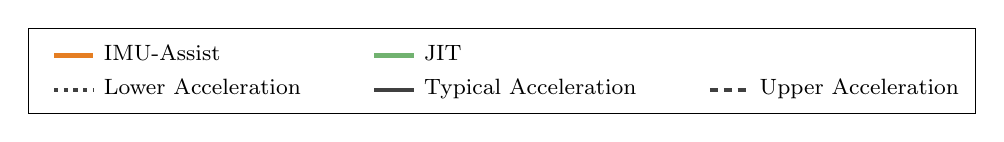
\begin{tikzpicture}
    \node[
        draw=black, line width=0.25pt,
        inner sep=3pt, rounded corners=0pt, align=center
    ] {%
        \footnotesize
        \setlength{\tabcolsep}{0pt}
        \renewcommand{\arraystretch}{1.3}
        \begin{tabular*}{\dimexpr0.95\linewidth}{
            c @{\extracolsep{0pt}\hspace{3pt}} l
            @{\extracolsep{\fill}}
            c @{\extracolsep{0pt}\hspace{3pt}} l
            @{\extracolsep{\fill}}
            c @{\extracolsep{0pt}\hspace{3pt}} l
        }
            \legline{cb_orange}{solid} & IMU-Assist &
            \legline{cb_green}{solid} & JIT & 
            & \\
            \legline{gray!50!black}{dotted} & Lower Acceleration &
            \legline{gray!50!black}{solid} & Typical Acceleration &
            \legline{gray!50!black}{densely dashed} & Upper Acceleration \\
        \end{tabular*}
    };
    \end{tikzpicture}}

    \caption{Mean capacity vs.\ IMU sampling period $T_{\text{IMU}}$, Ideal Mechanical steering ($d_{\text{link}}=\SI{3}{m}$). Bold lines mark the Lower, Typical, and Upper Acceleration values: $0.5$, $9.5$, and $20$ m/s$^2$ (translational); $0.5$, $300$, and $700$ deg/s$^2$ (rotational); vertical dashed lines mark the Table~2 baseline $T_{\text{IMU}} = \SI{10}{ms}$.}
    \label{fig:reb_robustness}
\end{figure}


\noindent JIT's performance also depends on the IMU sampling period $T_{\text{IMU}}$, which limits the evaluation rate of the trigger condition (Eq.~7). Sweeping $T_{\text{IMU}}$ from $\SI{0.5}{\milli\second}$ to $\SI{300}{\milli\second}$ under translational and rotational mobility (Fig.~\ref{fig:reb_robustness}), mean capacity is flat for both IMU-Assist and JIT up to $T_{\text{IMU}} \approx \SI{10}{\milli\second}$, with faster sampling providing marginal benefits. As $T_{\text{IMU}}$ increases, both algorithms degrade, but JIT retains a clear margin at low acceleration because coordinated AP/UE realignment tolerates a longer prediction window than unilateral IMU-Assist correction. The $\SI{10}{\milli\second}$ baseline sits at the edge of the plateau under both mobility patterns. We have also added this analysis to the \emph{Methods/JIT Beam Realignment} subsection of the manuscript.


%-------------------------------------------------------------------%
\begin{tcbremark}
{\fontfamily{cmss}\selectfont
\blue{Explain how the edge of coverage is defined and whether it adapts to UE speed or rotation. Also describe how the UE detects approaching EoC to transmit IMU data.}
}
\end{tcbremark}

\noindent The edge of coverage (EoC) is the $\pm\,\theta_{\text{HPBW}}/2$ off-boresight angle at which the antenna gain has dropped by \SI{3}{\deci\bel}. JIT places its trigger boundary inside the EoC, at the offset where the projected angular displacement over $T_{\text{react}}$ equals $\eta\,\theta_{\text{HPBW}}$; this boundary contracts toward boresight as motion speed grows and relaxes outward when motion slows. The projected displacement is evaluated locally at the UE from EWMA-filtered IMU samples and the antenna's known $\theta_{\text{HPBW}}$, so no AP-side feedback is required. A new \emph{Trigger Boundary and Edge of Coverage} subsubsection at the head of \emph{Methods/JIT Beam Realignment} states this in full; the new passage is reproduced below for convenience.

\begin{quote}
{\color{cyan!75!black}
The EoC is the angle off the AP's beam axis at which the antenna gain has dropped by \SI{3}{\deci\bel}, i.e., $\theta_{\text{HPBW}}/2$ off boresight. Crossing the EoC corresponds to a worst-case \SI{6}{\deci\bel} round-trip gain loss, particularly punishing in sub-THz where narrow, high-gain beams leave little SNR margin, and can directly cause link failure. Because reaching the EoC under mobility leaves no time for control signaling, JIT instead places a \emph{trigger boundary} inside the EoC, at the offset where the projected displacement during the system reaction time $T_{\text{react}}$ would reach $\eta \cdot \theta_{\text{HPBW}}$. The boundary adapts to motion: as the UE's Link Deviation Velocity $\|\dot{\boldsymbol{\delta}}\|$ grows, the projected displacement reaches $\eta \cdot \theta_{\text{HPBW}}$ at a smaller angular offset from boresight, so the trigger fires earlier, farther inside the EoC. When motion slows, the boundary moves outward toward the EoC, suppressing unnecessary control frames. For AP-stationary scenarios (e.g., a wall-mounted access point serving mobile UEs), detection of approaching EoC is performed locally at the UE: at every IMU sample, the UE evaluates Eq.~(7) using its body-frame kinematics and the known $\theta_{\text{HPBW}}$ of its own antenna, requiring no AP-side feedback. In future work, mobile-AP cases (e.g., UAV-borne access points) would extend the protocol so the AP also shares its kinematic state via the same control frame.
}
\end{quote}

\bigskip
\noindent We sincerely thank the Editor for these comments, which together have produced a clearer and more rigorous presentation of JIT's design rationale, parameter sensitivity, and operating range.

\newpage

%-------------------------------------------------------------------%
\section*{Reviewer 1}
\markboth{Reviewer 1}{}

\begin{tcbremark}
{\fontfamily{cmss}\selectfont
\blue{The novelty is meaningful, but its boundary relative to prior sensor-assisted/predictive beam management remains under-specified. \dots\ A clearer related-work positioning would strengthen the innovation claim.}
}
\end{tcbremark}

\noindent We agree, and have expanded the related-work positioning in the manuscript and added Table~\ref{tab:reb_relatedwork} placing JIT against six families of prior beam-management work. What is new in JIT is the combination of UE-side IMU motion sensing, a pre-failure trigger that anticipates the next beam-edge crossing, and coordinated AP/UE realignment delivered via a single in-band sub-THz control frame; to our knowledge, no prior work combines all three within a single sub-THz protocol with hardware-in-the-loop validation.\\

\noindent The per-family limitations are as follows. 3GPP NR Beam Failure Recovery~\cite{Giordani2018ATO, Heng2021SixChallenges} sends a discrete PRACH-based recovery message only after the MAC entity has counted $N$ consecutive Beam Failure Instances at L1. RF-based proactive failure prediction~\cite{9838772, Alrabeiah2020DeepLearning} forecasts a failure from RF time-series or sub-6\,GHz features and uses no motion sensing. AP-side multimodal sensing~\cite{Alkhateeb2023DeepSense, Jiang2023LiDAR, Morais2023Position} requires LiDAR, radar, vision, or GPS hardware at every AP. UE-side orientation-based work~\cite{Rezaie2022Orientation, Struye2023CoVRage} uses orientation primarily for codebook selection rather than to anticipate the next edge crossing. Continuous IMU streaming~\cite{Brambilla_2019} exchanges IMU data on every tracking interval over an out-of-band channel. Bilateral pilot-driven coordination~\cite{Alkhateeb2018DLCB, Xue2023Standardization} incurs overhead regardless of link risk.\\

\noindent By contrast, JIT sends one short in-band frame only when a crossing is imminent, for an overhead of less than $0.4\%$.\\

\noindent The two reactive baselines (Hierarchical Search and IMU-Assist) remain in the experimental comparison because they share JIT's protocol-level scope; Static and Perfect Alignment provide lower and upper reference bounds. The other approaches in Table~\ref{tab:reb_relatedwork} operate at a different protocol scope (standardized post-failure recovery, AP-side LiDAR/GPS, periodic bilateral pilots), and in-depth comparison against any of them is left for future work. The \emph{Discussion} future-work paragraph now lists this explicitly; the new passage is shown below for reference.

\begin{quote}
{\color{cyan!75!black}
\dots\ the validation scope can broaden toward (i)~multi-AP scheduling with handover, (ii)~non-line-of-sight channel models with multipath and transient blockage events, (iii)~HIL trials in which both nodes translate through azimuth and altitude, (iv)~sustained continuous-mobility scenarios with complementary bias-tracking mechanisms beyond the present initial-event focus, and (v)~larger-scale measurement campaigns spanning realistic indoor and outdoor environments.
}
\end{quote}

%-------------------------------------------------------------------%
\begin{tcbremark}
{\fontfamily{cmss}\selectfont
\blue{Insufficient tuning transparency, sensitivity analysis, and ablation make the source of JIT's gains hard to interpret.\dots}
}
\end{tcbremark}

\noindent Following the Reviewer's request, we have conducted a parameter-sensitivity analysis of both reactive baselines and of JIT itself. Three parameters were swept and compared against mean capacity: the spiral growth factor $\gamma$ for Hierarchical Search (Fig.~\ref{fig:reb_tuning_hs}), the refinement step factor $\beta$ for IMU-Assist (Fig.~\ref{fig:reb_tuning_imu}), and the guard fraction $\eta$ for JIT (Fig.~\ref{fig:reb_tuning_jiteta}). Additionally, the effect of the IMU sampling period $T_{\text{IMU}}$ is addressed in our response to the next remark. Each sweep uses the translational ($0.5$--$20$~m/s$^2$) and rotational ($0.5$--$700$~deg/s$^2$) peak-acceleration ranges present in the manuscript, with $n = 5{,}000$ Monte-Carlo runs per data point. The full sweep is drawn as faint background lines and the Lower, Typical, and Upper Acceleration values ($0.5$, $9.5$, $20$~m/s$^2$ translational; $0.5$, $300$, $700$~deg/s$^2$ rotational) are highlighted as bold lines.\\

\noindent Fig.~\ref{fig:reb_tuning_hs} shows the sensitivity of Hierarchical Search to changes in $\gamma$. For Hierarchical Search, $\gamma$ controls the geometric expansion of successive scan rings around the last known-good direction, since $HS_k = HS_0\,\gamma^k$. Sweeping $\gamma$ from $1.0$ to $2.0$, mean capacity peaks near $\gamma \approx 1.25$ under both mobility patterns. Tighter spacing ($\gamma \to 1$) keeps rings packed close together, covering angular distance too slowly to recover alignment within the beam residence time at higher accelerations; wider spacing ($\gamma > 1.4$) grows rings too quickly between steps and the search can skip past the optimal direction. The chosen $\gamma = 1.25$ sits at the trade-off optimum and remains within $\pm 10\%$ of the peak across the full acceleration range.\\

\noindent For IMU-Assist, $\beta$ scales the local refinement spiral step ($IA_k = \beta\,\theta_{\text{HPBW}} + \Delta\theta^{\star}$) that corrects residual error between the IMU-predicted angle and the true beam direction. Sweeping $\beta$ from $0.05$ to $0.55$ (Fig.~\ref{fig:reb_tuning_imu}) identifies a peak near $\beta \approx 0.10$: below $0.05$, the step is smaller than the residual error and the spiral does not converge within the beam residence time; above $0.15$, the first correction overshoots and the beam takes longer to align. The chosen $\beta = 0.10$ likewise stays within $\pm 10\%$ of the peak across the full acceleration range.\\

\noindent Finally, Fig.~\ref{fig:reb_tuning_jiteta} shows the sensitivity of JIT to changes in $\eta$. For JIT, $\eta$ controls how far inside the Edge of Coverage the control frame is fired via the trigger condition $\|\dot{\boldsymbol{\delta}}\| \cdot T_{\text{react}} > \eta \cdot \theta_{\text{HPBW}}$. Sweeping $\eta$ from $0.1$ to $0.7$ (Fig.~\ref{fig:reb_tuning_jiteta}), mean capacity stays within $\pm 5\%$ of its maximum across the plateau $\eta \in [0.25, 0.50]$. Below $\eta = 0.20$, the trigger fires too frequently and signaling overhead climbs sharply; above $\eta = 0.50$, the realignment is delayed and the UE drifts further off-axis before correcting. The chosen $\eta = 0.36$ sits at the center of this plateau.\\

\noindent Even at the baselines' own optima ($\gamma = 1.25$: \SI{38.3}{Gbps}; $\beta = 0.10$: \SI{47.8}{Gbps}), JIT at $\eta = 0.36$ leads by at least $24$\,Gbps (\SI{71.7}{Gbps}) at typical translational acceleration, so the gain reflects the coordination mechanism rather than a favourable parameter choice for any of the schemes.

%-------------------------------------------------------------------%
\begin{tcbremark}
{\fontfamily{cmss}\selectfont
\blue{Several key engineering assumptions are under-analyzed.\dots\ However, it remains unclear how robust the proactive trigger is under longer continuous operation without reliable zero-velocity intervals.\dots\ The effect of this sensing timescale on trigger freshness and prediction accuracy is not adequately analyzed.}
}
\end{tcbremark}

\noindent JIT's robustness to long-term IMU drift depends on the IMU characteristics and the user's movement profile. Short bursts of motion allow opportunistic zero-velocity update (ZUPT) corrections that bound the bias, but in sustained continuous mobility without ZUPT opportunities the accumulated drift would otherwise degrade an IMU-only predictor over time. However, two design choices aim to mitigate this issue:\\

\noindent First, a pre-failure trigger,
\begin{equation}
    \|\dot{\boldsymbol{\delta}}\| \cdot T_{\text{react}} > \eta \cdot \theta_{\text{HPBW}}, \tag{Eq.~7}
\end{equation}
uses the Link Deviation \emph{velocity} $\|\dot{\boldsymbol{\delta}}\|$, requiring only a single accelerometer integration rather than the double integration of position-based predictors. The integrated quantity therefore accumulates drift linearly rather than quadratically with time. Despite this mitigation, we acknowledge that long-term drift would still degrade an the IMU predictor over time in sustained continuous mobility without ZUPT opportunities. 

To avoid fully relying on the IMU, JIT utilizes the RF link measurements to aid the IMU, in cases of long-term drift. The RF link provides closed-loop verification at every algorithm iteration, and a localized Hierarchical Search runs whenever the IMU-based prediction underestimates a beam-edge crossing. Thus, any residual misalignment caused by drift is detected and corrected on the RF side rather than left silent.\\

\noindent To further improve robustness, for sustained continuous-mobility scenarios that lack rest intervals (e.g., a pedestrian walking continuously, or a vehicle in steady transit), complementary bias-tracking from the inertial-navigation literature such as learning-based dead-reckoning~\cite{Brossard2020AIIMU}, deep-learning drift compensation~\cite{Chen2024DLInertial}, or zero-velocity detection~\cite{Skog2010ZUPT} would augment JIT's calibration as future work. This is additionally added to our \emph{Discussion} future-work paragraph.\\

\noindent Additionally, in order to better understand the effects of trigger freshness and prediction accuracy, we have swept the IMU sampling period $T_{\text{IMU}}$ from $\SI{0.5}{\milli\second}$ to $\SI{300}{\milli\second}$ under translational and rotational mobility (Fig.~\ref{fig:reb_robustness}). Mean capacity is flat for both IMU-Assist and JIT up to $T_{\text{IMU}} \approx \SI{10}{\milli\second}$, with faster sampling providing only marginal benefits. As $T_{\text{IMU}}$ increases, both algorithms degrade, but JIT retains a clear margin at low acceleration because coordinated AP/UE realignment tolerates a longer prediction window than unilateral IMU-Assist correction. This analysis is now added to the \emph{Methods/JIT Beam Realignment} subsection of the manuscript; the new passage is reproduced below for reference.

\begin{quote}
{\color{cyan!75!black}
Figure 9 sweeps the IMU sampling period $T_{\text{IMU}}$ for both IMU-Assist and JIT under translational and rotational mobility. Mean capacity is flat up to $T_{\text{IMU}} \approx \SI{10}{\milli\second}$, so faster sampling adds no benefit. Beyond this point both algorithms degrade, but JIT retains a clear margin at low acceleration: coordinated AP/UE realignment tolerates a longer prediction window than unilateral IMU-Assist correction. By $T_{\text{IMU}} = \SI{300}{\milli\second}$ this margin collapses, as the inter-sample angular increment exceeds what one realignment can recover.
}
\end{quote}


%-------------------------------------------------------------------%
\begin{tcbremark}
{\fontfamily{cmss}\selectfont
\blue{The current validation scope remains simplified (single AP--single UE, predominantly LoS/FSPL-based modeling, and HIL constrained to the azimuth plane), which limits the external validity of some design insights, such as the robustness and low-overhead operation of JIT.}
}
\end{tcbremark}

\noindent We thank the Reviewer for raising this point. We agree that the present study is first-order, and the manuscript frames it as such in the \emph{Discussion} (``the presented first-order evaluation results\dots''). The single-link, predominantly LoS setup was chosen to isolate the beam-management mechanism from multi-AP, NLoS, and larger-scale effects. However, we note the scope have listed the corresponding extensions are as future work in the revised \emph{Discussion}: multi-AP scheduling with handover, non-LoS channels with multipath and blockage, full-3D HIL with both nodes translating in azimuth and altitude, sustained continuous-mobility scenarios, and larger-scale indoor/outdoor measurements.\\

\noindent We would also like to clarify HIL constraints. The dual-axis rotary stages support full 3D antenna pointing in both azimuth and altitude, so the HIL beam pointing and all of the algorithms were operating in 3D. The constraint is only on the linear translation of the RF front-end mounts, which limit the variety of motions, increasing test-to-test variation. However, our experimental results utilized both altitude and azimuth parts of the algorithms presented. 

With our sub-terahertz testing hardware, each front-end is too heavy to lift vertically, so the linear translation is restricted to the azimuth plane. This is now stated explicitly in \emph{Statistics and Reproducibility} and acknowledged in the \emph{Discussion} future-work paragraph (item iii). The new sentence is reproduced below.

\begin{quote}
{\color{cyan!75!black}
The dual-axis rotary stages support full 3D antenna pointing in both azimuth and altitude; the linear translation of the RF front-end mounts, however, was constrained to the azimuth plane by the weight of the RF equipment.
}
\end{quote}

%-------------------------------------------------------------------%
\begin{tcbremark}
{\fontfamily{cmss}\selectfont
\blue{The ``Link Deviation Velocity'' $\dot{\boldsymbol\delta}$ in equation~(6) combines UE angular velocity and LoS-perpendicular translational velocity divided by distance. It would benefit from a clearer explanation of how these quantities are represented and combined in the 3D coordinate frame, especially whether both terms are projected onto the same beam-deviation angular coordinates.}
}
\end{tcbremark}

\noindent Thank you for pointing this out and we agree that the coordinate convention needs clarification, and have made it explicit. Both terms in the Link Deviation Velocity,
\begin{equation}
    \dot{\boldsymbol{\delta}} = \boldsymbol{\omega}_{\text{UE}} + \frac{\mathbf{v}_{\perp}}{d_{\text{link}}}, \tag{Eq.~6}
\end{equation}
are expressed in the AP-anchored world coordinate frame via the UE orientation quaternion $\mathbf{q}_{\text{body}}$, so rotational and LoS-perpendicular translational contributions sum consistently as a single 3D angular rate. Two clarifying sentences have been added immediately after Eq.~(6) in \emph{Methods/JIT Beam Realignment}, and a complete notation summary has been added as a new Table~3 at the head of \emph{Methods}. The two new sentences are duplicated here for reference.

\begin{quote}
{\color{cyan!75!black}
Both terms in Eq.~(6) are expressed in the AP-anchored world coordinate frame: the UE's body-frame angular velocity $\boldsymbol{\omega}_{\text{UE}}$ and translational velocity perpendicular to the LoS, $\mathbf{v}_{\perp}$, are transformed via the UE's orientation quaternion $\mathbf{q}_{\text{body}}$ (the same quaternion that contributes to $\mathbf{q}_{\text{eff}}$ in the antenna pattern evaluation discussed below). This common frame ensures that rotational and LoS-perpendicular translational contributions to beam deviation are summed consistently as a single 3D angular rate.
}
\end{quote}

%-------------------------------------------------------------------%
\begin{tcbremark}
{\fontfamily{cmss}\selectfont
\blue{In the subsection of JIT Beam Realignment, the derivation of the filtered acceleration trend $\bar{\mathbf{a}}_{\text{predict}}$ from EWMA needs further explanation.}
}
\end{tcbremark}

\noindent We noticed that this was not clearly explained and have revised \emph{Methods/JIT Beam Realignment} subsection to now state the recurrence explicitly as
\begin{equation}
    \bar{\mathbf{a}}_{\text{predict},k} = \alpha_{\text{short}}\, \mathbf{a}_k + (1 - \alpha_{\text{short}})\, \bar{\mathbf{a}}_{\text{predict},k-1},
\end{equation}
with $\alpha_{\text{short}} = 0.90$ as listed in Table~2. This low-pass cutoff suppresses high-frequency IMU sensor noise while preserving the underlying acceleration trend, which the AP uses to extrapolate the UE's position at steering completion.

%-------------------------------------------------------------------%
\begin{tcbremark}
{\fontfamily{cmss}\selectfont
\blue{The Perlin smootherstep function in equation~(8) mathematically forces velocity and acceleration to zero at keyframe boundaries. While this is reasonable for generating smooth trajectories, the authors should explain why this is an adequate approximation for the considered mobility scenarios.}
}
\end{tcbremark}

\noindent We thank the Reviewer for prompting this clarification, which has been added after the smootherstep equation in \emph{Methods}. The trajectories model pause-resume actions such as walking between two points (Fig.~\ref{fig:translational_rate}) and rotating in place by \SI{90}{\degree} (Fig.~\ref{fig:rotational_rate}). These trajectories also enable controlled, reproducible evaluation, with each scenario allowing the variation of a single parameter (e.g., peak acceleration). To further illustrate combined motion profiles, the Combined Motion scenarios (Fig.~\ref{fig:antenna_comparison}) use both translation and rotation with varying end times, mirroring real actions such as taking a step while turning the head. This makes the trajectories less predictable but more representative of real-world motion. These clarifications have been added in \emph{Methods}; the relevant passage is reproduced below.

\begin{quote}
{\color{cyan!75!black}
The zero-velocity boundary models pause-resume mobility, the primary motion class in this study (walking with intermediate stops, or beginning and ending a turn from rest). Such single-component trajectories also support a controlled evaluation in which a single parameter (e.g., peak acceleration) is varied per scenario, and the same trajectory replays in both the simulator and the HIL testbed. Translational and rotational components use independent keyframes, so the combined-motion scenarios (Sec.~\ref{sec:combined_motion}) can have rotation in progress while translation is at rest (or vice versa), producing trajectories that are less predictable but more representative of real-world motion (e.g., taking a step while turning the head). The platform also supports sustained trajectories (e.g., continuous walking through multiple checkpoints) by chaining segments with non-zero endpoint velocities while preserving slot-by-slot $C^1$ continuity.
}
\end{quote}

%-------------------------------------------------------------------%
\begin{tcbremark}
{\fontfamily{cmss}\selectfont
\blue{Equations~(12) and~(13) explicitly model the E-plane pattern of the WR-6.5 horn, but it is not clear whether the 3D kinematic simulation assumes a rotationally symmetric pattern based on the E-plane.}
}
\end{tcbremark}

\noindent The Reviewer's interpretation is correct. The assumption is now stated immediately after the Fresnel-arguments equation in \emph{Methods}. The new text is duplicated here.

\begin{quote}
{\color{cyan!75!black}
For 3D evaluation, the radiation pattern is treated as rotationally symmetric about the boresight: the gain $G(\theta)$ depends only on the off-axis angle $\theta$ obtained by transforming the 3D LoS vector into the antenna's local frame via $\mathbf{q}_{\text{eff}}$, and the E-plane formula above is applied across all azimuth angles around boresight as a rotationally symmetric approximation. The HIL measurements cross-check this approximation against the physical horn and confirm that it is sufficient for this evaluation.
}
\end{quote}

\bigskip
\noindent We sincerely thank Reviewer~1 for the careful read and thoughtful comments, which together have led to a clearer and more rigorous presentation of the methods and evaluation scope.

\newpage

%-------------------------------------------------------------------%
\section*{Reviewer 2}
\markboth{Reviewer 2}{}

\begin{tcbremark}
{\fontfamily{cmss}\selectfont
\blue{The setting of the ``trigger boundary'' in the JIT method is not well explained. Specifically, how is EoC determined, and will it be adjusted based on the user's speed or rotation?}
}
\end{tcbremark}


\red{STILL TODO FIGURE AND REDO THIS ONE}

\noindent The edge of coverage (EoC) is the $\pm\,\theta_{\text{HPBW}}/2$ off-boresight angle at which the antenna gain has dropped by \SI{3}{\deci\bel}. Crossing the EoC corresponds to a worst-case \SI{6}{\deci\bel} round-trip gain loss, which is particularly punishing in sub-THz where narrow, high-gain beams leave little SNR margin and the link can fail outright. Because reaching the EoC under mobility leaves no time for control signaling, JIT places an inner \emph{trigger boundary} inside the EoC, at the offset where the projected angular displacement during the system reaction time $T_{\text{react}}$ would reach $\eta\,\theta_{\text{HPBW}}$:
\begin{equation*}
    \|\dot{\boldsymbol{\delta}}\| \cdot T_{\text{react}} > \eta \cdot \theta_{\text{HPBW}}. \tag{Eq.~7}
\end{equation*}
The guard fraction $\eta$ controls how aggressively the trigger fires; its sensitivity sweep (Fig.~\ref{fig:reb_tuning_jiteta}) is discussed in our response to Reviewer~1, Comment~2 above and identifies a plateau $\eta \in [0.25, 0.50]$ within which mean capacity stays within $\pm 5\%$ of the maximum.\\

\noindent The trigger boundary adapts to motion through the Link Deviation Velocity,
\begin{equation*}
    \dot{\boldsymbol{\delta}} = \boldsymbol{\omega}_{\text{UE}} + \frac{\mathbf{v}_{\perp}}{d_{\text{link}}}, \tag{Eq.~6}
\end{equation*}
which combines the UE's body-frame angular velocity $\boldsymbol{\omega}_{\text{UE}}$ and its translational velocity perpendicular to the LoS, $\mathbf{v}_{\perp}$, both expressed in the AP-anchored world frame via the orientation quaternion $\mathbf{q}_{\text{body}}$. Faster motion (larger $\|\dot{\boldsymbol{\delta}}\|$) contracts the trigger boundary toward boresight and fires the control frame earlier, farther inside the EoC; slower motion relaxes the boundary outward toward the EoC and suppresses unnecessary control frames. Both speed and rotation feed into Eq.~(7) through the same scalar: under pure rotation $\mathbf{v}_{\perp} \approx 0$ and the trigger fires off the angular-velocity term alone, while under pure translation $\boldsymbol{\omega}_{\text{UE}} \approx 0$ and it fires off the translational term alone. Mixed motion combines them coherently as a single 3D angular rate.\\


\noindent A new \emph{Trigger Boundary and Edge of Coverage} subsubsection at the head of \emph{Methods/JIT Beam Realignment} now formalizes this geometry in the revised manuscript.

%-------------------------------------------------------------------%
\begin{tcbremark}
{\fontfamily{cmss}\selectfont
\blue{Since the user is within the beam coverage, how can it determine that it is approaching the EoC in order to transmit its IMU message?}
}
\end{tcbremark}

\red{STILL TODO FIGURE AND REDO THIS ONE}

\noindent Detection is performed locally at the UE, without AP-side RF feedback. At every IMU sample the UE applies the ZUPT-derived biases to obtain $\mathbf{a}_{\text{corr}}, \boldsymbol{\omega}_{\text{corr}}$, transforms its body-frame velocities into the AP-anchored world frame via $\mathbf{q}_{\text{body}}$, computes $\dot{\boldsymbol{\delta}}$ using the last known-good $d_{\text{link}}$ from the RF link, and tests $\|\dot{\boldsymbol{\delta}}\| \cdot T_{\text{react}} > \eta\,\theta_{\text{HPBW}}$. All four required quantities are available on the UE side (IMU readings, orientation quaternion, last known link distance, and the antenna's $\theta_{\text{HPBW}}$), so the UE can predict the future EoC crossing from its own kinematic state and transmit a control frame before the link is lost.\\

\noindent Three mechanisms keep this UE-local prediction reliable in the presence of IMU impairments: the trigger uses velocity rather than position to avoid double-integration drift; opportunistic ZUPT bounds the residual bias; and the SNR-driven fallback at \SI{9.59}{\deci\bel} reverts the system to the Hierarchical Search baseline if the IMU-based prediction underestimates the crossing, so the link is never lost silently.\\

\noindent For mobile-AP cases (e.g., UAV-borne access points), the same control frame is the natural carrier for the AP's kinematic state; this extension is on the future-work list.

%-------------------------------------------------------------------%
\begin{tcbremark}
{\fontfamily{cmss}\selectfont
\blue{System configurations and KPI definitions should be introduced before the results section to enhance the readability of the Results. Please restructure the paper for better clarity.}
}
\end{tcbremark}

\noindent Following the Reviewer's suggestion, the opening of \emph{Results} has been restructured: the four reference schemes, the three steering models, and the four KPIs are now grouped under a new labelled subsection at the head of \emph{Results}, with full derivations left in \emph{Methods/Evaluation Metrics}. The new subsection heading and its opening are included below.

\begin{quote}
{\color{cyan!75!black}
\textbf{Experimental Setup and Performance Metrics.} We benchmark JIT against four reference schemes\ldots\ We evaluate each scheme across four key performance indicators (KPIs)\ldots: \emph{Mean Capacity} ($\bar{C}$)\ldots; \emph{Capacity Coefficient of Variation (CoV)}\ldots; \emph{Link Availability} ($A_{\text{link}}$)\ldots; and \emph{Signaling Overhead} ($O_{\text{sig}}$)\ldots
}
\end{quote}

%-------------------------------------------------------------------%
\begin{tcbremark}
{\fontfamily{cmss}\selectfont
\blue{On page 3, when referring to the ``state-of-the-art beam recovery approach (without IMU assistance),'' it is unclear which specific work this refers to. Please provide a reference and more details about this approach.}
}
\end{tcbremark}

\noindent We thank the Reviewer for pointing this out; the original phrasing was indeed ambiguous. The intended comparator is the IEEE~802.11ad / 3GPP~NR-style hierarchical sequential beam search, and the \emph{Results} preamble now names it explicitly and cites the relevant prior work. The same citations have been added in \emph{Methods/Hierarchical Search} where the spiral pattern is introduced. The IMU-assisted baseline now also cites the mmWave IMU-assisted beam-tracking literature in \emph{Methods/IMU-Assisted Reactive Search}. The updated sentence from the \emph{Results} preamble is reproduced below.

\begin{quote}
{\color{cyan!75!black}
We benchmark JIT against four reference schemes. The first two are: (i)~a state-of-the-art Hierarchical Search beam recovery approach (without IMU assistance)~\cite{photonics11060540}, consistent with the SSB-based beam search defined for 3GPP NR~\cite{Giordani2018ATO, Heng2021SixChallenges}; and (ii)~a reactive IMU-assisted beam alignment (leveraging IMU data for beam realignment, but without JIT signaling)~\cite{s141019622, Brambilla_2019, 9391649}.
}
\end{quote}

%-------------------------------------------------------------------%
\begin{tcbremark}
{\fontfamily{cmss}\selectfont
\blue{In Figure~2, the JIT method shows trends that seem to contradict the IMU-assisted approach at high acceleration. What limitations in the JIT method explain this divergence from IMU-assisted performance? In contrast, in Figure~4, why does JIT match the IMU trend in the electronic model? Please explain the differences and the reasons behind this phenomenon.}
}
\end{tcbremark}

\noindent We agree that the trends differ across the two figures, and this reflects a real difference in mechanism rather than a JIT limitation. The AP's optimal action under rotation is different from its optimal action under translation, and JIT and IMU-Assist reach those optima through different paths.\\

\noindent \textbf{Rotation (Fig.~\ref{fig:rotational_rate}, Electronic model).} Under pure rotation, the UE's position in the AP-anchored world frame does not change; only its orientation rotates. The optimal response is for the UE to counter-rotate while the AP holds its boresight on the original LoS. Under Electronic steering, the UE-side counter-rotation completes within microseconds, so IMU-Assist tracks even \SI{700}{deg/s^2} and the AP observes only minor transient RF fluctuations rather than a sustained power drop; the AP therefore does not typically initiate a reactive scan, and effectively converges to the correct behavior of holding its boresight. 

JIT reaches the same outcome, informing the AP via the in-band control frame that the motion is purely rotational so that the AP holds its boresight by design. Both algorithms therefore produce the same qualitative trend in this regime. JIT still retains a consistent lead of approximately \SI{19}{Gbps} across the acceleration range (Fig.~\ref{fig:rot_simfast_rate}), avoiding the IMU-Assist overshoot and improving false-reactive scans, discussed in \emph{Methods/IMU-Assisted Reactive Search}.\\

\noindent \textbf{Translation (Fig.~\ref{fig:translational_rate}).} Under translation, the UE's position in the AP's frame changes, so both nodes must steer to maintain alignment. IMU-Assist applies its local IMU-based prediction at the UE without communicating with the AP; the AP, lacking access to IMU information, relies on its RF pipeline alone to react. 

JIT instead transmits an in-band control frame to coordinate the AP-side update, which incurs a finite reaction latency $T_{\text{react}} = T_{\text{frame}} + T_{\text{proc}} \approx \SI{15}{\micro\second}$ that IMU-Assist's purely local correction does not pay. At low-to-moderate translational accelerations, JIT's pre-failure coordination provides the largest mean-capacity advantage because the AP can be aimed at the predicted future position before RF degradation occurs. At higher accelerations under Electronic steering (Fig.~\ref{fig:trans_simfast_rate}, \SIrange{10}{20}{m/s^2}), $T_{\text{react}}$ becomes a constraint and both algorithms approach the same physical limit set by the beam residence time; the mean-capacity gap narrows to roughly $12\%$ (JIT \SI{72.6}{Gbps} vs IMU-Assist \SI{63.4}{Gbps}). However, JIT continues to lead on other metrics such as capacity CoV (Fig.~\ref{fig:trans_metrics_covariance}), where its preemptive coordination keeps the instantaneous capacity more stable than the reactive baselines.

%-------------------------------------------------------------------%
\begin{tcbremark}
{\fontfamily{cmss}\selectfont
\blue{In Figure~3, after beam alignment, why is there a power deviation compared to the ``perfect alignment'' case? What does this deviation represent? Why does JIT's trajectory information not seem to assist in perfectly aligning the beam after realignment?}
}
\end{tcbremark}

\noindent We appreciate the careful read of Fig.~3 and we would like to clarify that the residual gap is intentional rather than a realignment shortcoming. JIT only triggers a realignment when the projected misalignment is about to cross the trigger boundary (Eq.~7), while the Perfect Alignment reference assumes zero misalignment at every instant. A new paragraph in \emph{Results} now explains this; and it is also reproduced below.

\begin{quote}
{\color{cyan!75!black}
A small residual gap between JIT and the Perfect Alignment reference is visible in the steady-state portion of Fig.~3. By design, JIT does not continuously chase the maximum SNR; it triggers realignment only when the projected angular displacement is about to cross $\eta \cdot \theta_{\text{HPBW}} = 0.36 \cdot \SI{13}{\degree} \approx \SI{4.7}{\degree}$ (Eq.~7). Between triggers, the UE may sit slightly off-axis without correction, while the Perfect Alignment reference assumes zero misalignment at every instant.
}
\end{quote}

\bigskip
\noindent We sincerely thank Reviewer~2 for the close reading of the figures, which has prompted us to articulate JIT's event-triggered behavior and the figure-to-figure consistency more clearly than in the original submission.

\newpage

%-------------------------------------------------------------------%
\noindent We sincerely thank the Editor and the Reviewers for the thoughtful and constructive feedback, which has substantially improved the clarity and rigor of the manuscript. We hope the revisions adequately address every concern raised, and we look forward to your further consideration.\\

\noindent Sincerely,\\

\noindent Sergey Petrushkevich, Vitaly Petrov, and Josep~M.~Jornet

\printbibliography

\end{document}
